\documentclass[11pt,titlepage,twoside]{scrreprt}
\usepackage[bottom=3.5cm]{geometry}
\usepackage[english]{babel}
\usepackage[applemac]{inputenc}

\usepackage{tgtermes}
\usepackage[T1]{fontenc}
\usepackage[lite,subscriptcorrection,slantedGreek,nofontinfo]{mtpro2}

\usepackage[automark]{scrlayer-scrpage}
\usepackage{mathtools}
\usepackage{graphicx}
\usepackage{amsthm}
\usepackage{amssymb}
\usepackage{amsmath}
\usepackage{extarrows}
\usepackage{esint}
\usepackage{faktor}
\usepackage{tikz-cd}
\usepackage{commath}
\usepackage{enumitem}
\usepackage[intoc]{nomencl}
\usepackage{titlesec, blindtext, color}
\usepackage{tocloft}
\usepackage{todonotes}
\usepackage{listings}
\usepackage{siunitx}
\usepackage{dsfont}
%\usepackage{pstricks,pst-node,pst-tree}

%\usepackage{bold-extra}
\usepackage{algpseudocode,algorithm,algorithmicx}

\renewcommand{\cfttoctitlefont}{\normalfont\bfseries\Huge}
\usepackage[intoc]{nomencl}

\makenomenclature
\renewcommand{\nomname}{Nomenclature}

\usepackage[pdftex,plainpages=false]{hyperref}

\renewcommand{\baselinestretch}{1.3}

%\newcommand*\DNA{\textsc{dna}}

%\newcommand*\Let[2]{\State #1 \(\gets\) #2}
\algrenewcommand\algorithmicrequire{\textbf{Input:}}
%\algrenewcommand\algorithmicensure{\textbf{Postcondition:}}

\begin{document}

\newtheoremstyle{defstyle}
{}              %Space above    
{}              %Space below
{}                      %Body font: original {\normalfont}    
{}                      %Indent amount (empty = no indent,%\parindent = paraindent)    
{\normalfont\bfseries}  %Thm head font original 
{.}{10pt}      
{{\scshape\bfseries \thmnumber{#2}\thmname{ #1}\thmnote{ (#3)}}}
\newtheoremstyle{satzstyle}
{}              %Space above    
{}              %Space below
{\itshape}                      %Body font: original {\normalfont}    
{}                      %Indent amount (empty = no indent,%\parindent = paraindent)    
{\normalfont\bfseries}  %Thm head font original 
{.}{10pt}      
{{\scshape\bfseries \thmnumber{#2} \thmname{ #1}\thmnote{ (#3)}}}
\newtheoremstyle{emptystyle}
{}              %Space above    
{}              %Space below
{}                      %Body font: original {\normalfont}    
{}                      %Indent amount (empty = no indent,%\parindent = paraindent)    
{\scshape\bfseries}  %Thm head font original 
{.}{6pt}      
{{\scshape\bfseries \thmnumber{#2}\thmnote{ #3}}}

\theoremstyle{satzstyle}
\newtheorem{satz}{Satz}[chapter]
\newtheorem{theo}[satz]{Theorem}
\newtheorem{lem}[satz]{Lemma}
\newtheorem{kor}[satz]{Korollar}
\newtheorem{cor}[satz]{Corollary}
\newtheorem{folg}[satz]{Folgerung}
\newtheorem{prop}[satz]{Proposition}
\theoremstyle{defstyle}
\newtheorem{defi}[satz]{Definition}
\newtheorem{bem}[satz]{Bemerkung}
\newtheorem{rem}[satz]{Remark}
\newtheorem{bsp}[satz]{Beispiel}
\newtheorem{ex}[satz]{Example}
\theoremstyle{emptystyle}
\newtheorem{emp}[satz]{}

\renewcommand*{\thesatz}{\arabic{chapter}.\arabic{satz}}
\renewcommand*{\theequation}{\arabic{chapter}.\arabic{equation}}
\renewcommand{\labelenumi}{\textup{(\textit{\roman{enumi}})}}
%\newcommand{\hsp}{\hspace{20pt}}
\titleformat{\chapter}[display]{\huge\bfseries}{Chapter \thechapter}{20pt}{\Huge\bfseries}
\titleformat{\section}{\Large\bfseries}{\thesection}{7pt}{}
\titleformat{\subsection}{\large\bfseries}{\thesubsection}{5pt}{}
\titleformat{\subsubsection}{\large\scshape\bfseries}{\thesubsubsection}{5pt}{}
\renewcommand{\cfttoctitlefont}{\bfseries\Huge}
\renewcommand\cftchapfont{\bfseries}
\renewcommand\thechapter{\textup{\Roman{chapter}}}
%\renewcommand\headmark{\thechapter}

\deftripstyle{custom}{\textsc{\headmark}}{}{\textsc{\pagemark}}{}{}{}

\pagenumbering{roman}

\begin{titlepage}

\begin{center}

\vspace*{1cm}

%\renewcommand{\baselinestretch}{2}

{\Huge Parameter estimation and consistency for \\[.2cm] discrete %\\[.2cm] 
determinantal point processes}\\[1cm]
% Inference for determinantal point processes � from point estimators to a Bayesian setting 

{\Large Dissertation submitted for the degree of}\\%[.2cm]
{\Large\textsc{Master of Science in Interdisciplinary Mathematics}}\\[.5cm]
{\Large Johannes M�ller}\\[.3cm]

{\Large \today}\\[3.8cm]


\includegraphics[width=0.25\textwidth]{figures/crest_black}\\[1cm]

\textsc{Supervised by}\\%[.1cm]
\textsc{\Large Professor Nikolaos Zygouras and Dr Theodoros Damoulas}\\[.6cm]
%
\includegraphics[width=0.45\textwidth]{./the_warwick_uni_black}\\[.3cm]
\textsc{\huge University of Warwick}\\[.1cm]
\textsc{\LARGE Department of Mathematics}%\\[3.5cm]
\vfill
\end{center}
\end{titlepage}

\cleardoublepage

\begin{center}
{\LARGE\textsc{Acknowledgements}\\[.9cm]}
% \normalsize
\begin{minipage}{11cm}
%I would like to thank the dreamteam for being such an eggcelent friendgroup and for all the pun we had during the last year.
\end{minipage}
\end{center}

\clearpage


\begin{center}
{\LARGE\textsc{Abstract}\\[.9cm]}
\begin{minipage}{11cm}
%Determinantal point processes are random subsets that exhibit a diversifying behaviour in the sense that the randomly selected points tend to be not similar in some way. This repellent structure first arrose in theortical physics and pure mathematics, but they have recently been used to model a variety of many real world scenarios in a machine learning setup. We aim to give an overview over the main ideas of this approach which is easily accessible even without prior knowledge in the area of machine learning and sometimes omit technical calculations in order to keep the focus on the concepts.
Determinantal point processes (DPPs) are a probabilistic model of diverse subsets that exhibits desirable computational properties in terms of its simulation, marginalisation and other operations. That is why they have recently been used in an increasing amount of real world applications like text summarisation and the selection of a diverse subset of pictures returned by an image search (cf. \cite{kulesza2012learning}). A crucial step in all of those applications is the estimation of different parameters and therefore this will be the focus of this dissertation. We will give an overview over two different point estimators and their benefits and hindrances and provide proofs for their consistency. We will see that the main drawback of the maximum likelihood estimation is that it results in the maximisation of the log likelihood function which is not concave in the case of DPPs and therefore not possible in an efficient way. This motivates the Bayesian approach to the estimation of those parameters and we see how the posterior density can be approximated using different Markov chain Monte Carlo (MCMC) methods.
\end{minipage}
\end{center}

%\todo{cite, or give more obvious examples}{ }

\clearpage


\pagestyle{custom}
\cleardoublepage
\setlength{\cftchapnumwidth}{10mm}
\tableofcontents
\cleardoublepage
\pagenumbering{arabic}

%\manualmark \markboth{}{Nomenclature}
\nomenclature{\(\operatorname{sgn}\)}{Either the sign of a number or the parity of a permutation.}

\nomenclature{\(\mathbb Z_2\)}{The cyclic group consisting of \(\left\{ 0, 1\right\}\) with the addition modulo \(2\).}

\nomenclature{\(\mathbb F_2\)}{The finite field \(\left\{ 0, 1 \right\}\) with the addition and multiplication modulo \(2\).}

\nomenclature{\(\mathbb N\)}{The natural numbers.}

\nomenclature{\(\mathbb R\)}{The real numbers.}

\nomenclature{\(D^2f\)}{Hessian matrix, i.e. second derivative of a function \(f\colon\mathbb R^d\to \mathbb R\).}

\nomenclature{\(\mathbb R^d\)}{The Euclidean \(d\)-dimensional space with Euclidean norm \(\left\lVert \cdot \right\rVert\).}

\nomenclature{\(L^2(\mu)\)}{The space of square integrable functions with scalar product \[(\phi, \psi)_{L^2(\mu)} = \int\phi(x)\psi(x)\mu(\mathrm dx).\]}

\nomenclature{\(\mathbb R^{N\times N}_{\text{sym}, +}\)}{The set of non negative definite symmetric \(N\times N\) matrices.}

\nomenclature{\(\mathbb R_+\)}{The set of non negative real numbers \([0, \infty)\).}

\nomenclature{\(O(g(x))\)}{We write \(f(x) = O(g(x))\) if \(f(x) \le M g(x)\) for all \(x\ge x_0\) and one \(M>0\).}

\nomenclature{\(\operatorname{span}\)}{This denotes the span of a collection of vectors.}

\nomenclature{\(A\ge B\)}{We write \(A\ge0\) if \(A\) is non negative definite and \(A\ge B\) if \(A-B\ge 0\) where \(A\) and \(B\) are symmetric matrices.}

\nomenclature{\(\arg\max\)}{The \(\arg\max\) function selects one arbitrary maximiser given it exists.}
\printnomenclature[2.5cm]{}

\chapter*{Introduction}
%\chapter*{Preface}
%\addtocontents{toc}{Preface}
\addcontentsline{toc}{chapter}{Introduction}
\manualmark \markboth{}{Introduction}


%\section{Motivation}

%\todo{explain why DPPs are awesome}

%\section{Previous work}

%\section{Aim and outline of the dissertation}

%This dissertation emerged from the 



Before we introduce determinantal point processes (DPPs) mathematically we should give a short motivation for their study as well as an overview over the dissertations and its contributions. It is the goal to give a mostly self contained presentation to different approaches for the parameter estimation for DPPs that is accessible to any student familiar with the basic notions of linear algebra, analysis and probability theory. We prove most statements of this dissertation or give precise references if the statements are not assumed to be (mathematical) general knowledge.

\subsubsection*{Motivation}

Determinantal point processes are point processes, i.e. random subsets that exhibit a diversifying, repulsive behaviour in the sense that the subset is likely to obtain only elements that are different in some way. They arose first as the distribution of the eigenvalues of random matrices in \cite{mehta1960density} and later on in theoretical physics as the positions of Fermions like positively charged \(\alpha\)-particles that repell themselves (cf. \cite{benard1973detection}). Since then, they have appeared in the study of different random objects like non intersecting random walks and the descent positions in a random digit sequence (cf. \cite{johansson2004determinantal} and \cite{borodin2010adding}). The Wigner hypothesis states that the energy levels at which a neutron is scattered or reflected by a heavy nuclei are distributed according to a DPP (cf. \cite{tao2010universality}). Furthermore, DPPs arise in number theory as it has been conjectured that the positions of the non trivial roots of the Riemannian zeta function are distributed according to a determinantal point process (cf. \cite{bourgade2013quantum}). Hence, DPPs are fundamental to different theories and are therefore highly interesting objects and a rich mathematical theory has been developed for them (cf. \cite{borodin2009determinantal}, \cite{hough2006determinantal}, \cite{lyons2003determinantal}).
In recent years DPPs have also been used to treat different real world phenomena and we will only present three of them shortly here.
\begin{enumerate}
\item \emph{Image search}: Assume we have given a set of \(10^6\) pictures that were returned by a search engine for a particular query. On the first page only a few, lets say \(20\) can be presented and in order to increase the probability that the user is satisfied with at least one picture it is favourable to include pictures that are not very similar in some notion. This can be modelled by a DPP since the goal is to select a diverse subset of pictures (cf. \cite{kulesza2011k}). % however one has to estimate 
\item \emph{Text summarisation:} DPPs have also been used successfully for extractive summarisation of news articles. The task of extractive summarisation is to select a subset of the sentences in order to obtain a reasonable summary of the text. The reason for the use of DPPs -- or any other diversifying point process -- is that similar sentences should not be selected for the summary since it would be quite repetitive then and hence one of the sentences should rather not be included in the summary (cf. \cite{kulesza2012learning1}). 
\item \emph{Pose selection:} Maybe the most fascinating application of DPPs has been found in the task of human pose extraction. The goal is -- given an image with an unknown amount of persons -- to schematically select their poses. A pose is associated with a quadrupel of rectangles which represent the head, torso and the two arms of a person. Since a picture consists of a finite number of pixels, the number of possible poses is also finite. It is possible to model how likely a certain pose is to be actually present in a given picture. If one would sample naively according to those probabilities one runs into the following problem: Similar poses usually have almost the same probability since they should describe the actual pose just about equally well. Hence, naive approaches are likely to select more than one of those poses for the same human.
\begin{figure}[h!]
	\centering
	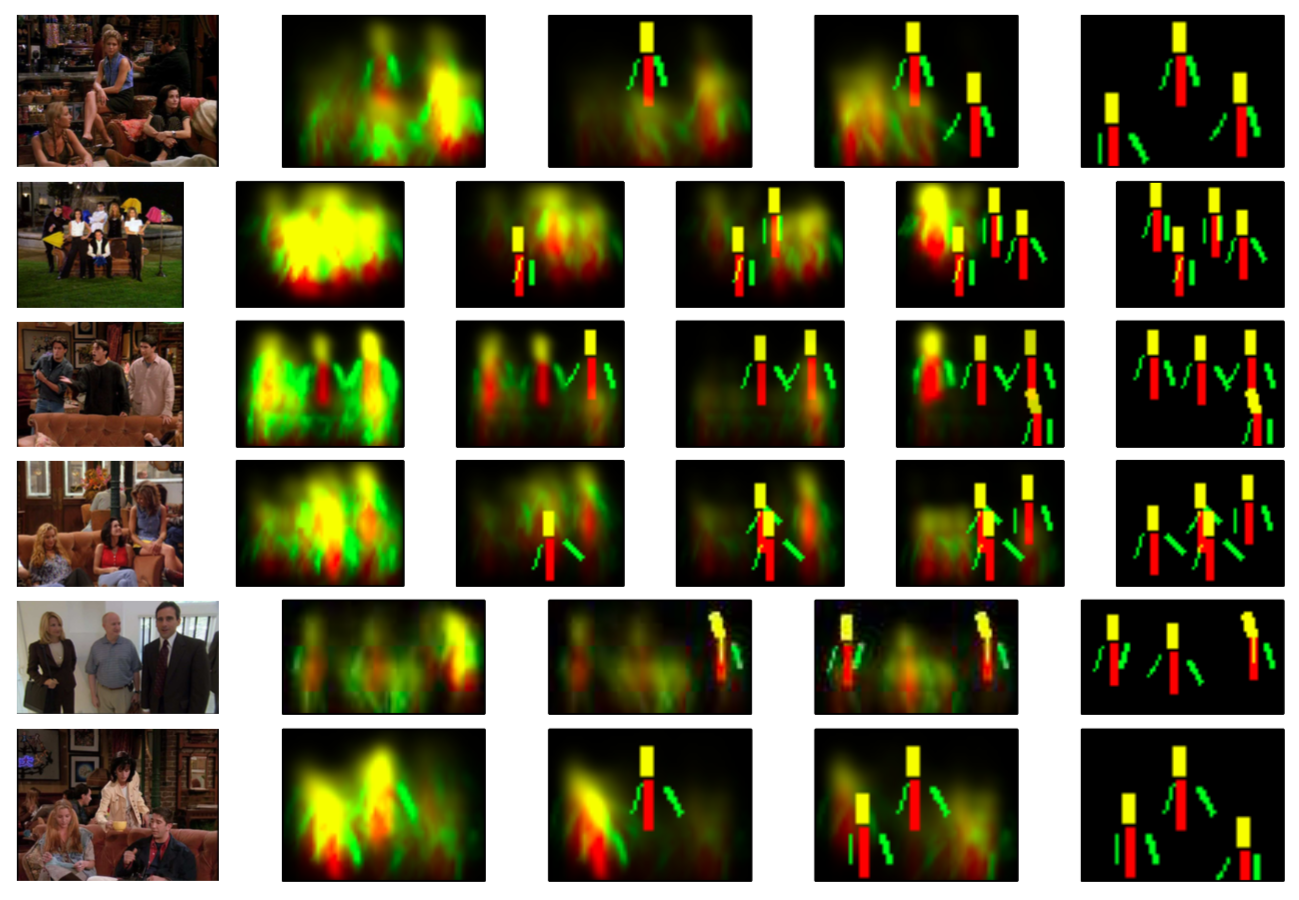
\includegraphics[width=0.99\textwidth]{figures/pose-estimation}
	\caption{The successive selection of poses in picture using a DPP based on a the quality of the poses which is depicted in the second column. Original graphic due to \cite{kulesza2010structured}.}
	\label{fig:1}
\end{figure}
 This is where the repellent structure of a DPP can help in order to make it unlikely to select similar poses which leads to the effect that in most cases only one pose is selected for one person in the picture. This approach has successfully been taken in \cite{kulesza2010structured} and made it possible to perform the pose selection without the knowledge of the number of persons present in the picture.
\end{enumerate}

%In practice the procedure in those real world applications can be divided into two parts, the first one being the modelling of some properties of the phenomenon, the second one being the estimation of certain parameters. We will focus on the second part, since it is universal to a lot of real world applications and can be put into rigorous terms.
The procedure of the application of DPPs to those and further real world problems can roughly be divided into two parts. The first one consists of the selection of a suitable model for the given task and the second one of the estimation of 
%A crucial step in the application of DPPs to those and further real world problems is to estimate 
different parameters of the DPP which will be the focus of this dissertation. % and hence it is of great interest how this can be done.

%\section{Historical remarks}
%\begin{enumerate}
%\item Theoretical work:
%\begin{enumerate}
%\item DPPs are point processes, i.e. random (locally finite) subsets that exhibit a diversifying, repulsive behaviour.
%\item They first arose as the positions of Fermions, for example positively charged \(\alpha\)-particles that repell themselves spatially or eigenvalues of random matrices.
%\item They continue to appear in
%\begin{enumerate}
%\item the study of many different random events like non intersection random walks and ...
%\item theoretical physics like the spectra of stars ...
%\item other areas of mathematics, for example the non trivial roots of the Riemmannian zeta function are conjectured to are distributed according to a DPP.
%\end{enumerate}
%\end{enumerate}
%\item In recent years DPPs have been used in the study of different real world phenomena including
%\begin{enumerate}
%\item Text summarisation
%\item Image search
%\item Pose estimation
% \item Applications to clustering
% \item Applications in computer vision (pose estimation special case)
%\end{enumerate}
%\item In practice the procedure in the procedure in those real world applications can be divided into two parts, the first one being the modelling of some properties of the phenomenon, the second one being the estimation of certain parameters. We will focus on the second part, since it is universal to a lot of real world applications and can be put into rigorous terms.
%\item All of applications include the estimation of the (some) parameters of the DPP and hence we will focus on this
%\end{enumerate}

\subsubsection{Outline of the thesis}
In the first chapter we introduce discrete determinantal point processes and present the fundamental concepts we will need. Further, we show that for a given marginal kernel a corresponding DPP exists and see how DPPs can be simulated and apply this to some toy examples. In the second chapter we will present two different ways how an estimator can be obtained for the marginal kernel or parametrisations of it. We will see that both strategies yield a consistent estimator. In the last chapter we will present the fundamentally different Bayesian approach to parameter estimation and apply it to the estimation of parameters of DPPs. In order to do this in practice we have to make use of Markov chain Monte Carlo (MCMC) methods and hence provide a minimalistic introduction to those.
The appendix contains a collection of some statements used in the thesis and also the R code that was used for the simulation of DPPs and also the parameter estimations that where performed.

\subsubsection{Contributions}
The dissertation is mainly built around the PhD thesis \cite{kulesza2012learning} and the research initiated by it, however, we provide a few novelties. We present a completely self contained presentation of the estimator of the marginal kernel that was first proposed in \cite{urschel2017learning} and give a different, arguably easier proof for the consistency of this estimator. Furthermore, we will provide proofs for the consistency of the maximum likelihood estimators for different parametric models of DPPs that could not be found in the literature so far.\footnote{At least to the best knowledge of the author.} In the last chapter we give a short introduction to MCMC methods including a collection of its mathematical foundations that is shorter -- and of course not as comprehensive -- than in most text books. We hope that the given toy examples help the understanding of DPPs and the influence of the different parameters to its properties. The provision of the code could save some people some time, although it should be mentioned that most algorithms will be far from computationally optimal.


%\begin{enumerate}
%\item Outline:
%\begin{enumerate}
%\item Chapter I: Basics that we need to investigate the task of parameter estimation including the existence and simulation of DPPs and some toy examples.
%\item Chapter II: Presentation of two different point estimators including the proof of consistency of both.
%\item Chapter III: Discussion of a Bayesian framework for parameter estimation in general and for DPPs specifically including the benefits of this approach.
%\end{enumerate}
%\item Contributions:
%\begin{enumerate}
%\item Give a self contained presentation of the estimator for the marginal kernel that is presented in ... including a different, arguably easier proof of the consistency
%\item Show that the MLEs for different parameters exist with increasing probability and are in fact consistent.
%\item Give a short introduction into Bayesian parameter estimation and MCMC methods with a presentation of the mathematical foundations of those.
%\item Provide easy examples throughout the thesis including simulation and parameter estimations for those. The code for this is also included in the appendix.
%\end{enumerate}
%\item It is the aim to give a mostly self contained approach to the topic that is accessible to any student familiar with basic notions of linear algebra, analysis and probability theory. We proof almost everything we use in this dissertation or give precise references if the statements are not (mathematical) general knowledge.
%\end{enumerate}

%\automark % \markboth{}{Introduction}

\chapter{Determinantal point processes: Basic notions and properties}
%\chapter{Introduction to discrete determinantal point processes}

In this chapter we provide %a short motivation for the topic itself and 
an overview over the basic notions and results for discrete determinantal point processes. Those will be necessary to study the problem of parameter estimation later on. First we rigorously introduce the concept of discrete determinantal point processes and define the most important subclass that we will work with a lot later. This is exactly the subclass where one can express the elementary probabilities of the point process nicely. This will be crucial later on if one wants to perform the parameter estimation based on elementary probabilities, like for example maximum likelihood estimation or Bayesian parameter estimation.

Then we will turn towards the question of existence and simulation of determinantal point processes. This will lead to an algorithm that samples from a DPP which we will use to built some toy examples and also to generate the data sets we will perform parameter estimation for in the following chapters.

\section{Definitions and properties}

We begin by presenting the general frame we will work in. This means that we will keep the notation introduced here and will use those objects throughout the thesis without further explanation. We will present all the important properties of determinantal point processes that we will need but omit some calculations that have been presented somewhere else and don�t contribute to a better understanding of the topic. A much more in depth survey of properties of determinantal point processes including extensive comparisons to several other point processes can be found in the report \cite{kulesza2012determinantal}.%\todo{comment on continuous DPPs at one point!}

\begin{emp}[Setting]
Let \(\mathcal Y\) be a finite set, which we call the \emph{ground set} and \(N\coloneqq \left\lvert \mathcal Y \right\rvert\) its cardinality. We call the elements of \(\mathcal Y\) \emph{items } and assume for the sake of easy notation \(\mathcal Y = \left\{ 1, \dots, N\right\}\) unless otherwise specified. %\coloneqq\left\{ 1,\dots, N\right\}\). 
A \emph{point process} on \(\mathcal Y\) is a random subset %\(\mathbf Y\) 
of \(\mathcal Y\), i.e. a random variable with values in the powerset \(2^{\mathcal Y}\). We will identify this random variable with its law\footnote{The law of a random variable is just the push forward measure of the probability measure of the probability space the random variable is defined on.} \(\mathbb P\) and thus refer to probability measures \(\mathbb P\) on \(2^{\mathcal Y}\) as point processes and will not distinguish between those objects. Further, \(\mathbf Y\) will always denote a random subset distributed according to \(\mathbb P\).
\end{emp}

\begin{defi}[Determinantal point process]
We call \(\mathbb P\) a \emph{determinantal point process}, or in short a \emph{DPP}, if we have
\begin{equation}\label{e2.1}
\mathbb P(A\subseteq \mathbf Y) = \det(K_A) \quad \text{for all } A\subseteq \mathcal Y
\end{equation}
where \(K\) is a symmetric matrix indexed by the elements in \(\mathcal Y\) and \(K_A\) denotes the submatrix 
\((K_{ij})_{ij\in A}\)
of \(K\) indexed by the elements of \(A\). We call \(K\) the \emph{marginal kernel} of the DPP. If the marginal kernel \(K\) is diagonal, we call \(\mathbb P\) a \emph{Poisson point process}.
\end{defi}

We note that all principal minors\footnote{The \emph{principle minors} of \(K\) are the determinants of the submatrices \(K_A\) for \(A\subseteq \mathcal Y\).} of \(K\) are necessarily non negative and Sylvester�s criterion implies that \(K\) is positive semi-definite.\footnote{\(K\) is called \emph{positive semi-definite} if \(x^TKx\ge0\) for all \(x\in\mathbb R^{\mathcal Y}\). The Sylvester criterion states that a matrix is positive semi-definite if and only if all principle minors are non negative.} Further it can be shown \footnote{This follows from equation (2.3) in \cite{borodin2009determinantal}.} that also the complement of a DPP is a DPP with marginal kernel \(I-K\) where \(I\) is the identity matrix, i.e.
\[\mathbb P(A\subseteq\mathbf Y^c) = \det(I_A-K_A).\]
Thus, we can conclude \(I-K\ge0\) and obtain \(0\le K\le I\). This actually turns out to be sufficient for \(K\) to define a DPP through \eqref{e2.1} which we will see in the fourth section of this chapter.%(cf. \cite{kulesza2012determinantal}).\todo{why? explain!}{ }

\begin{emp}[Repulsive behaviour of DPPs]
%We call the elements of \(\mathcal Y\) \emph{items } and 
If we choose \(A=\left\{ i\right\}\) and \(A=\left\{ i,j\right\}\) for \(i,j\in \mathcal Y\) in \eqref{e2.1} we obtain the probabilities of the occurrence of the items \(i\) and \(j\) %\(\mathbb P(i\in \mathbf Y) = K_{ii}\) and
\begin{equation}\label{e2.2}
\begin{split}
\mathbb P(i\in \mathbf Y) & = K_{ii} \quad \text{and} \\
% \quad \text{and }
\mathbb P(i,j\in\mathbf Y) & = K_{ii}K_{jj}-K_{ij}^2 = \mathbb P(i\in\mathbf Y)\cdot\mathbb P(j\in\mathbf Y)-K_{ij}^2.
\end{split}
\end{equation}
Thus, the appearances of the two items \(i\) and \(j\) are always negatively correlated. This negative correlation is exactly what causes the diversifying behaviour of determinantal point processes. %In practice one usually models the negative correlations to be high between items that are similar in some notion. For example in a spatial setting being similar could mean being close together and in this case the selected items would tend to be not very close together.
This repulsive behaviour can be seen in Figure \ref{fig:1}. %\todo{insert picture!}{ }
Note that Poisson point processes are exactly the DPPs without correlations of the points.

\begin{figure}[h!]
	\centering
	%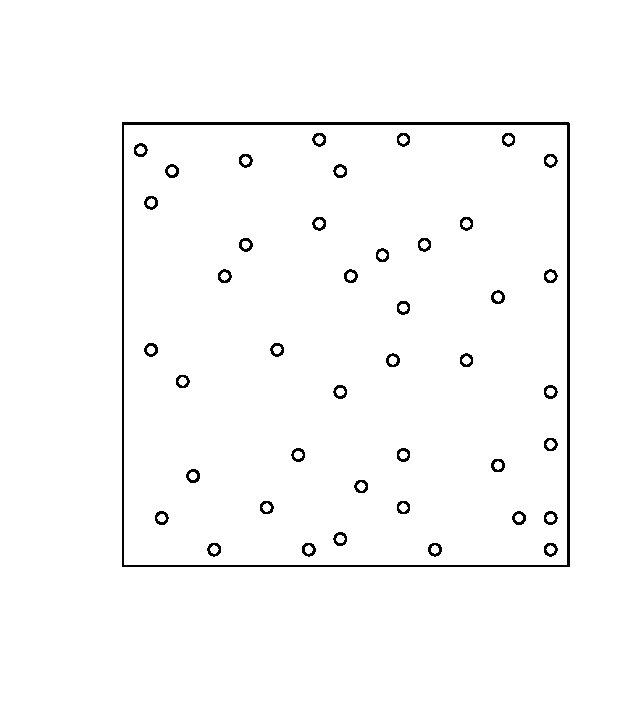
\includegraphics[width=0.44\textwidth]{DPP-in-square-2}
	%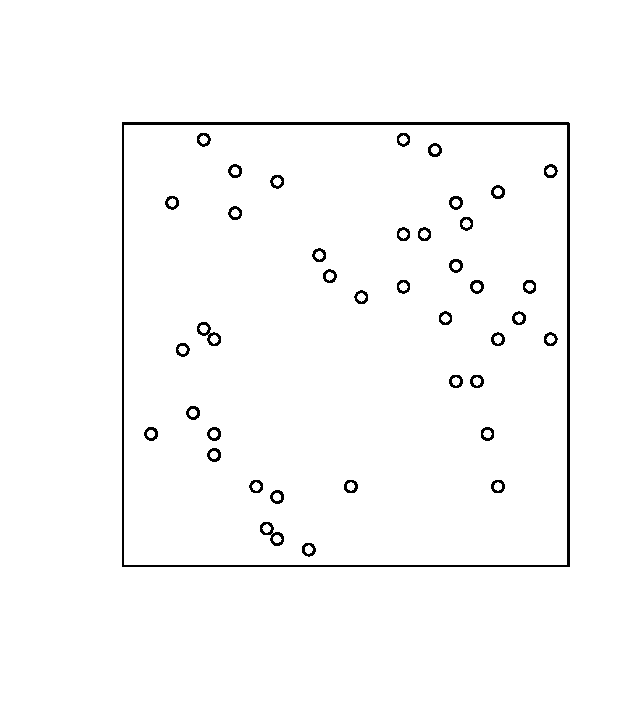
\includegraphics[width=0.44\textwidth]{Poisson-in-square-2}
	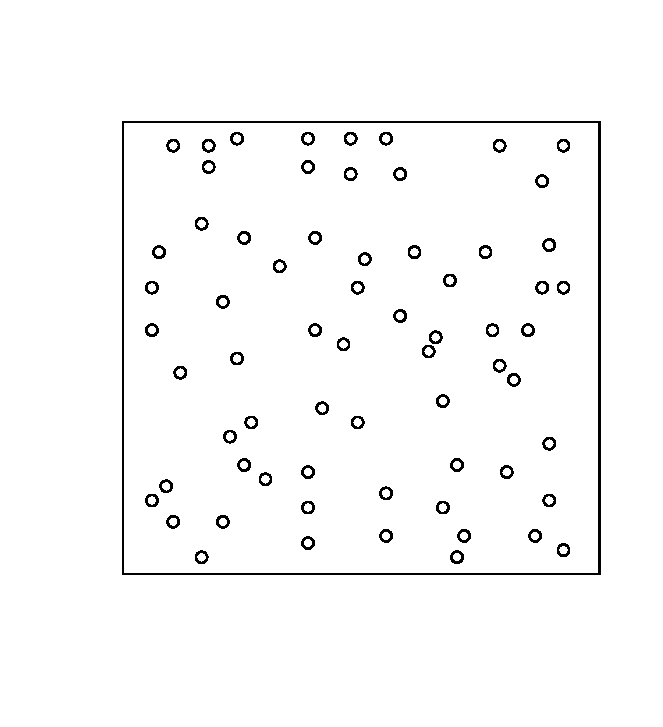
\includegraphics[width=0.444\textwidth]{figures/DPP-in-square-large-3}
	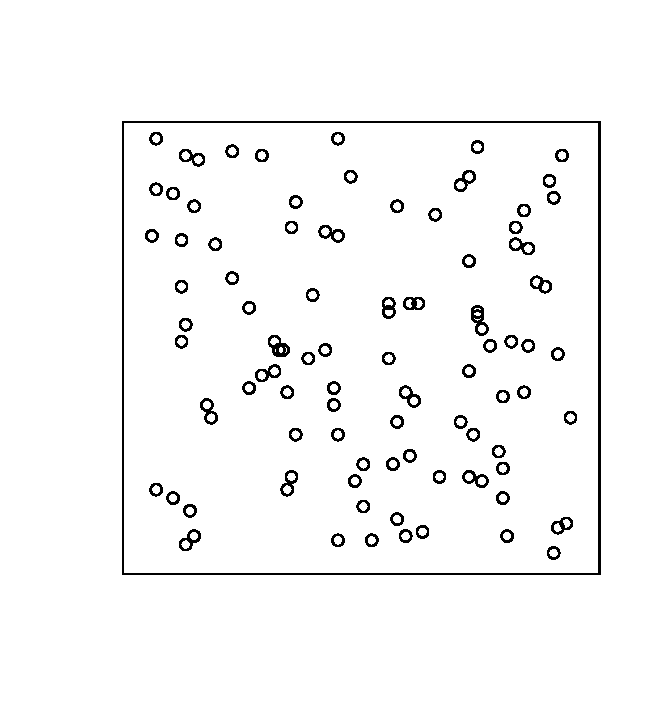
\includegraphics[width=0.44\textwidth]{figures/Poisson-in-square-large-2}
%	\tag{1}
	\caption{A DPP with negative correlations of close points on a \(100\times100\) grid in the unit square on the left and a Poisson point process on the same grid on the right with the same expected cardinality. The -- in this case spatially -- repellent structure of the DPP is clearly visible.}
	\label{fig:1}
\end{figure}

In this light the fact that also \(\mathbf Y^c\) exhibits negative correlations becomes less surprising. Since the set \(\mathbf Y\) tends to spread out due to the repulsion in \eqref{e2.2}, the complement, which is nothing but the gaps that are left after eliminating the elements in \(\mathbf Y\), tend to show a repulsive structure too.
\end{emp}

% \subsection*{\(L\)-ensembles}
\begin{emp}[\(L\)-ensembles]
Let us now introduce an important subclass of DPPs, namely the ones where not only the marginal probabilities can be expressed through a suitable kernel, but also the elementary probabilities. This will be convenient for us later when we will need expressions for the elementary probability in order to take a maximum likelihood approach\footnote{This will thoroughly be introduced in the next chapter.} to the estimation of certain parameters. If we have even \(K<I\), then we define the \emph{elementary kernel}
\begin{equation}\label{e2.2.1}
L\coloneqq K(I-K)^{-1}
\end{equation}
which specifies the elementary probabilities since one can check \footnote{This is done in full detail in \cite{kulesza2012learning} and we will not repeat those arguments here.}% \todo{make reference to appendix}
\begin{equation}\label{e2.3}
\mathbb P(A=\mathbf Y) = \frac{\det(L_A)}{\det(I+L)} \quad\text{for all } A\subseteq\mathcal Y.
\end{equation}
Conversely for any \(L\ge0\) a DPP can be defined via \eqref{e2.2} and the corresponding marginal kernel is given by the inversion of \eqref{e2.2.1}
\[K=L(I+L)^{-1}\]
and we have again \(K<I\). We call DPPs which arise this way \(L\)-\emph{ensembles}. %\todo{discuss equivalence to DPPs with \(\mathbb P(\emptyset)>0\)}
We will see in \ref{carDPP} that the cardinality of a DPP is distributed like the sum of \(N\) Bernoulli experiments with expectation \((\lambda_n)_{n=1, \dots, N}\) where \(\lambda_n\) are the eigenvalues of \(K\). Being an \(L\)-ensemble is equivalent to \(K<I\) which again is equivalent to \(\lambda_n<1\) for all \(n=1, \dots, N\) and hence equivalent to
\[\mathbb P(\mathbf Y = \varnothing) = \mathbb P(\left\lvert \mathbf Y \right\rvert = 0) > 0.\]
\end{emp}

\subsection*{The quality diversity decomposition}

We note that any symmetric, positive semi-definite matrix \(L\) can be written as a Gram matrix%\todo{explain this decomposition?}
\[L=B^TB\]
where \(B\in\mathbb R^{D\times N}\) whenever \(D\) is larger than the rank \(\operatorname{rk}(L)\) of \(L\). For example one could take the spectral decomposition \(L = U^TCU\) of \(L\) and set \(B\coloneqq \sqrt{C} U\) and eventually drop some zero rows from \(\sqrt{C}\). Let \(B_i\) denote the \(i\)-th column of \(B\) and we can write this as the product \(B_i = q_i\cdot \phi_i\) where \(q_i\ge0\) and \(\phi_i\in\mathbb R^D\) such that \(\left\lVert \phi_i \right\rVert=1\). This yields the representation
\[L_{ij} = q_i \phi_i^T\phi_j q_j \eqqcolon q_i S_{ij}q_j\]
and we call \(q_i\) the \emph{quality} of the item \(i\in \mathcal Y\) and \(\phi_i\) the \emph{diversity feature vector} of \(i\) and \(S\) the \emph{similarity matrix} or \emph{similarity kernel}. Since we will use this decomposition multiple times, we fix its properties. % and \(S_{ij}\coloneqq\phi_i^T\phi_j\in[-1,1]\) the \emph{similarity} of the two items \(i\) and \(j\). %Further we call \(\phi_i\) the \emph{diversity feature vector} of the element \(i\).\todo{comment on \(L\) ensembles} %, which will be further explained by the later examples.

\begin{prop}[Quality diversity parametrisation]
Let \(D\in\mathbb N\) and let \(\mathbb S_D\) denote the sqhere in \(\mathbb R^D\). 
Further let \(\mathbb R^{N\times N}_{\text{sym}, +}\) be the set of symmetric positive semi-definite \(N\times N\) matrices. 
The quality diversity parametrisation is a continuous and surjective mapping %bijection
%\todo{its not a bijection!!!} %from the 
\[\Psi\colon\mathbb R_+^N\times \mathbb S_D^N \to \left\{L\in \mathbb R^{N\times N}_{\text{sym}, +} \;\big\lvert\; \operatorname{rk}(L)\le D \right\}, \quad (q, \phi) \mapsto \left( q_i\phi_i^T\phi_j q_j\right)_{1\le i, j\le N}. \]
\end{prop}

\begin{rem}
\begin{enumerate}
\item In the case \(D \ge N\) the quality diversity decomposition gives a parametrisation of the whole symmetric positive semi-definite \(N\times N\) matrices.
% \item One could argue that one should rather call the pseudo inverse of the described surection the quality diversity decomposition. However, the 
\item Note that this parametrisation is not unique, i.e. \(\Psi\) is not injective. For example the identity matrix \(I\) can be parametrised by any orthonormal system \(\phi\in\mathbb S_N^N\) and \(q = (1, \dots, 1)^T\).
\item One can without any problems consider diversity features \(\phi_i\) in an abstract Hilbert space \(\mathcal H\). However, we will not need this in the remainder and thus restrict ourselves to the easier case of Euclidean diversity features.
\item We call every preimage \((q, \phi)\) of \(L\) under \(\Psi\) \emph{quality diversity decomposition} of \(L\). Further, we call the tupel \(\phi\in \mathbb S_D^N\) of normalised vectors the \emph{diversity feature matrix}.
\end{enumerate}
\end{rem}


Not only will the quality diversity decomposition play a central role when it comes to the actual modelling of real world phenomena with DPPs. It will also provide some useful expressions like the following one for the elementary probabilies% will provide some useful expressions. For example the elementary probabilities take the form
\begin{equation}\label{e2.4}
\mathbb P(A=\mathbf Y) \propto \det\!\big((B^TB)_A\big) % = \det\!\big(\Psi(q, \phi)_A\big) 
= \left(\prod_{i\in A} q_i^2\right) \cdot \det(S_A) \quad \text{for all } A\subseteq\mathcal Y.
\end{equation}
% which turns out to be a very helpful expression of the elementary probabilities.%\todo{comment on advantages of choosing \(D\) small}

%An intuitive understanding of the quality diversity decomposition will play a central role in the modelling process of real world phenomena through DPPs.
%later on if one wants to model real world phenomena as DPPs.
% To get this %, we can identify an item \(i\in\mathcal Y\) with the vector \(B_i=q_i\phi_i\in\mathbb R^D\) and
In order to get an intuitive understanding of the quality diversity decomposition we can think of \(q_i\ge0\) as a measure of how important or high in quality the item is and the diversity feature vector \(\phi_i\in\mathbb R^D\) can be thought of as some kind of state vector that consists of internal quantities that describe the item \(i\) in some way. Further, we interpret the scalar product \(\phi_i^T\phi_j\in[0,1]\) as a measure of similarity between the items \(i\) and \(j\) which justifies the name similarity matrix for \(S\). Note that if \(i\) and \(j\) are perfectly similar or antisimilar, i.e. \(\phi_i^T\phi_j=\pm1\), then they can not occur at the same time, since
\[\mathbb P(i,j\in\mathbf Y) = \det\begin{pmatrix} 1 & \pm1 \\ \pm1 & 1 \end{pmatrix} = 0. \]
If we identify \(i\) with the vector \(B_i=q_i\phi_i\in\mathbb R^D\), we can obtain a geometric interpretation of \eqref{e2.4} since \(\det\!\big((B^TB)_A\big)\) is the squared volume that is spanned by the columns \(B_i, i\in A\), which is visualised in \ref{fig:2}. This volume increases if the lengths of the edges that correspond to the quality increase and decrease when the similarity feature vectors point into more similar directions.

%\vspace{2cm}
\begin{figure}[h!]
	\centering
	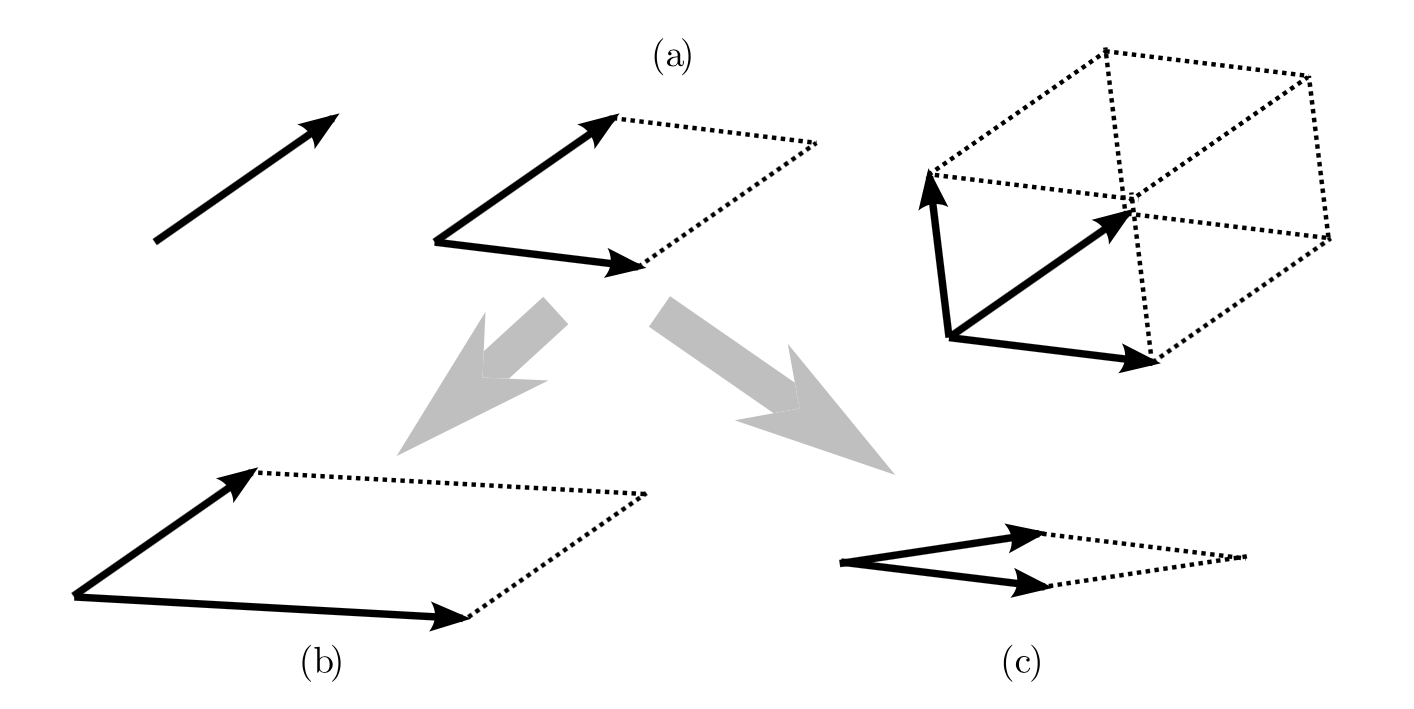
\includegraphics[width=0.8\textwidth]{figures/qd-decomposition}
%	\tag{1}
	\caption{The first line (a) illustrates the volumes spanned by vectors, and in the second line it can be seen how this volume increases if the length -- associated with the quality -- increases (b) and decreases if they become more similar in direction which we interpret as two items becoming more similar (c). Original graphic from \cite{kulesza2012determinantal}.}
	\label{fig:2}
\end{figure}

\begin{emp}[Modelling diversity over distance]\label{moddiv}
Since we will use one approach for the diversity features multiple times, we will now give a short general formulation of it. Let \(\mathcal R = \left\{ r_1, \dots, r_D\right\}\) be a finite set which we will call the \emph{reference set} and its elements the \emph{reference points}. Further, let
\[d\colon \mathcal Y\times \mathcal R\to\mathbb R_+, \quad f\colon\mathbb R_+\to \mathbb R\]
be mappings. Usually \(d(i, r)\) will be interpreted as a measure of distance between an item \(i\in\mathcal Y\) and a reference point \(r\in\mathcal R\) and will typically be given by a metric on a larger space that contains \(\mathcal Y\) and \(\mathcal R\).
One can now model \(\phi_i\in\mathbb R^{\mathcal R}\) via
\[(\phi_i)_r \propto f\!\big(d(i, r)\big) \quad \text{for } r\in\mathcal R.\] % j = 1, \dots, D. \]
The function \(f\) will typically be decreasing and thus \((\phi_i)_r\) can be seen as a measure of how similar item \(i\) is to the reference point \(r\in\mathcal R\). Thus, the diversity feature vector \(\phi_i\) stores how similar the item \(i\) is to all reference points and the scalar product \(\phi_i^T\phi_j\) will be close to one, if the items \(i\) and \(j\) have approximately the same degrees of similarity to the reference points. It shall be noted that the choice of the number \(D\) of reference points bounds the rank of the kernel \(L\) and therefore also the largest subset that occurs with positive probability. Indeed we have \(\operatorname{rk}(L)\le D\) and for \(A\subseteq\mathcal Y\) with more than \(D\) elements \(\det(L_A) = 0\) and therefore \(\mathbb P(A) = 0\).
In the last section of this chapter we will give examples where \(d\) is quite naturally a metric % in most cases, at least in the ones where \(\mathcal Y\) consists of %spatial positions or 
%points in a metric space. On the other hand 
and will see how
the choice of \(f\) is crucial for the strength of the repulsion.

Similar approaches for the modelling of the diversity feature vector have been taken in \cite{leeindividualness} and \cite{kulesza2010structured} and further the method of reference points has been used in \cite{bardenet2015inference} to obtain bounds for the elementary probabilities of a DPP.
\end{emp}
%\begin{emp}[Transitivity of repulsion]
%One last property of DPPs that we shall mention is the fact that the negative correlations of the DPP posses a transient property in the sense, that if \(i\) and \(j\) and \(j\) and \(k\) are %similar, then \(i\) and \(k\) are also similar. This is due to the fact
%\[\left\lVert \phi_i - \phi_j \right\rVert^2 = \left\lVert \phi_i \right\rVert^2 + \left\lVert \phi_j \right\rVert^2 - 2\phi_i^T\phi_j = 2(1-\phi_i^T\phi_j)\]
%and thus
%\[\sqrt{1-\phi_i^T\phi_k} = \frac12\left\lVert \phi_i - \phi_k \right\rVert\le\frac12\big(\left\lVert \phi_i - \phi_j \right\rVert + \left\lVert \phi_j - \phi_k \right\rVert\big) = \sqrt{1-\phi_i^T\phi_j} + \sqrt{1-\phi_j^T\phi_k}.\]\todo{reformulate that part!}
%\end{emp}
%recent\todo{say something about the transitivity of repulsion?}

\begin{emp}[Comparison to other point processes]
A wide variety of point processes has been studied and used in different applications and determinantal point processes are by far not the only point processes with negative correlations. For example every Poisson point process can be turned into a process with negative correlations by removing %some points of the selected subset. For example one could delete
 all points that lie within a certain distance of another point of the subset. Another well studied class of point processes are the so called \emph{Gibbs} or \emph{Markov point proccesses}. The elementary probabilities are given by 
\[\mathbb P(A) \propto \exp(-F(A))\]
where \(F\colon2^{\mathcal Y}\to\mathbb R\) is called the \emph{energy function} is interpreted as a measure of how unfavourable a subset \(A\subseteq\mathcal Y\) is.
%Those are defined through an energy function

Although some of those different classes of point processes with negative correlation posses nice theoretical properties they share one major drawback. In fact a lot computations and also the simulation of those point processes can not be performed efficiently. For example in the case of Gibbs point processes even the time needed for the computation of the normalisation constant%not even the normalisation constant
\[\sum_{A\subseteq\mathcal Y} \exp(-F(A)) \]
grows exponentially with \(N\) since it is the sum over an exponentially large set. However, the special structure of the determinant itself leads to the explicit expression in \eqref{e2.3} of the normalisation constant for DPPs and the computation time for the algebraic computation of it only grows like \(N^3\) or even slower for numerical approximations (cf. \cite{emiris2005improved})%recent\todo{cite}
. A more in depth comparison of different point processes including their descriptive power can be found in \cite{kulesza2012determinantal}.
%In most cases even the computation of the normalisation constant 
\end{emp}

% \section{\(L\)-ensembles}

\subsubsection*{The mode problem}

One general motivation for modelling is the hope that one can make predictions based on the selected model. If the model is of stochastic nature, like in our case, and if one wants to predict its outcome, there are a few possible approaches. The first and possibly simplest one would be to sample from this model. This relies on the intuition that a realisation of a random variable should be a rather typical example for the random event. Going one step further one could try to find the most likely outcome of the random variable, which is known as the mode problem.

\begin{emp}[The mode problem]
Let \(X\) be a random variable with values in some space \(\mathcal X\) and let \(f\) be the density of the distribution of \(X\) with respect to some reference measure. Then the \emph{mode} is the maximiser
\[\hat x = \underset{x\in\mathcal X}{\arg\max}f(x)\]
of the density if it exists. The search for the mode is called the \emph{mode problem}.
\end{emp}


Our motivation for finding the mode of a random variable was to make better predictions for it. This hope is based on the believe that the mode should be a typical realisation of the random variable. However, this is not generally the case and therefore one should be cautious with this intuition.
To see this we consider a random natural number with the following distribution
\[\mathbb P(\left\{ n\right\}) \coloneqq \begin{cases} \;0.1 \quad & \text{if } n = 20 \\\; 0.09 & \text{if } n = 0, 1, \dots, 9 \\\; 0 &\text{otherwise} \end{cases}. \]
Although \(20\) is the most likely elementary event, it is not a very typical outcome, since in \(90\%\) of the cases the random variable will have values in \(\left\{ 0, 1, \dots, 9\right\}\) and hence is far away from the mode of the distribution. Similar examples can easily be constructed for continuous distributions.%recent\todo{add histrogram?}
%It is clear that mode is \(0\) in this example, but it is not a very typical outcome of the random variable, since the majority of events is centered around \(10\).



%Consider for example the mixture of two independent Gaussian random variables
%\[0.1\cdot X + 0.9\cdot Y\] % \quad \text{where } X\sim N(0, 10), Y\sim N()\]
%where \(X\) is centered with variance \(10\) and \(Y\) has mean \(5\) with variance \(1\), the densities are shown in Figure ....\todo{check whether this gives the desired effect and plot the density!}{ } 

The mode problem can often be solved explicitely or at least numerically if the density \(f\) is a smooth function defined on a subset of \(\mathbb R^d\). However, in the case of DPPs we have to deal with the probability measure on a finite set and thus the mode problem is a discrete optimisation problem over the powerset \(2^{\mathcal Y}\). The exponential size of the powerset turns this into a very hard computational task and it has been shown that the time to compute the mode -- or even an event with more than \(\frac89\) its probability -- grows exponentially with the cardinality \(N\) of \(\mathcal Y\) (cf. \cite{kulesza2012determinantal}). However, some algorithms for the approximation of the mode have been proposed for certain classes of DPPs or for the goal to find a subset of at least \(\frac14\) of the probability of the mode. For more information on those approaches we refer to \cite{djolonga2014map} and \cite{gillenwater2012near}. % \todo{refer to other papers that do approximations?}
%This is in general very hard to solve and it has been shown in \todo{cite} that it is NP hard to do so or even approximate it upto a factor of \(\frac89\). However, there were still different strategies proposed and we will present some of them including their main ideas. \todo{do this!}


\section{Variations of DPPs} %: conditional DPPs, \(k\)-DPPs and structured DPPs}

In this section we will present some useful variations of determinantal point processes. They serve different purposes and we will shortly explain their individual benefits. %Although they are important in the actual application to real world scenarios, we will hardly discuss them any further in the following.

%\subsection*{Conditional DPPs}

\begin{emp}[Conditional DPPs]
A \emph{conditional DPP} is a collection of \(L\)-ensembles indexed by \(X\in\mathcal X\), where \(X\) is called the \emph{input} of the conditional DPP. Thus, for every \(X\in\mathcal X\) we get a finite set \(\mathcal Y(X)\) and a determinantal point process \(\mathbb P(\cdot| X)\) on \(\mathcal Y(X)\) which is given by the elementary kernel \(L(X)\), i.e.
\[\mathbb P(A\lvert X) \propto \det\left(L_A(X)\right) \quad \text{for all } A\subseteq\mathcal Y(X). \]
Further we denote the quality and diversity features of the conditional DPP by \(q_i(X)\) and \(\phi_i(X)\) respectively.

% Conditional DPPs can probably be understood the best way by giving an easy example. For this purpose we will extend our example above of the pseudo randomly selected points in a grid, but this time we don�t want to restrict ourselves to one specific grid size. Thus, we will consider the input space \(\mathcal X = \mathbb N\) where the input \(n\in\mathbb N\) gives the fineness of the grid, i.e.
% \[\mathcal Y(n)\coloneqq n^{-1}\cdot\big\{ 0, \dots, n\big\}^2. \]
% So this time \(\mathcal Y(n)\) is the equally spaced grid in \([0,1]^2\) with space \(n^{-1}\) between two grid lines and we have \(N(n)=\left\lvert \mathcal Y(n) \right\rvert = (n+1)^2\).
% We model the diversities \(\phi_i(n)\in\mathbb R^{N}\) in the exact analogue way, i.e.
% \[\phi_i(n)_j \propto \left\lVert i-j \right\rVert\quad \text{for all } i, j\in \mathcal Y(n) \]
% and the explicit expressions for them remain valid.

It is not immediately clear why one would want to model a family of DPPs as a conditional DPP rather than as 
% the scenario described above by a conditional DPP rather than by a 
separate DPPs. The reason for this is that one wants to estimate the kernels \(L(X)\) for every \(X\in \mathcal X\). With a naive approach one would need to observe each of the DPPs \(\mathbb P(\cdot| X)\) individually which is often not possible. Thus, one hopes 
%The reason for this is that we hope
 to not only memorise the kernels \(L(X)\) for every single input \(X\in\mathcal X\) but rather to estimate the mapping that assigns every input \(X\) its elementary kernel \(L(X)\). If one achieved this task, one would be able to simulate and predict a DPP that one has not observed so far just by the knowledge about some DPPs that belong to the same conditional DPP. 
%  based on some training set. 
Of course this can only work if we assume some regularity or a certain structure of the function \(L\) and we will see one approach how this can be done in the next chapter.%which we will do in the third chapter where we put those consideration into a precise framework.

In conclusion conditional DPPs are suitable for the extrapolation of parameter estimation between from observed to similar DPPs.
\end{emp}

%\subsection*{Fixed size or \(k\)-DPPs}
\begin{emp}[Fixed size or \(k\)-DPPs]
We have introduced DPPs as a model of random diverse subsets of a finite set. However, there are a lot of cases where the size of this subset is already known, like for example if the DPP models the position of football players on the field, we already know how many points we have to select, namely 11 -- at least if no player was sent off or got injured.

The straight forward procedure to obtain a probability distribution over all subsets of a fixed size that still propagates diversity is to condition a DPP on the event that it has this exact size. If we conditioned on the event that the point process has \(k\le N\) elements, we call this new point process \(k\)-DPP. Luckily \(k\)-DPPs possess similarly attractive properties like normal DPPs, in the sense that there is an analytical form of the normalisation constant as well as an effective sampling algorithm (cf. \cite{kulesza2011k}). Hence, \(k\)-DPPs allow to describe random diverse subsets of fixed size and one application for this will be discussed at the end of the next chapter.
\end{emp}

%\subsection*{Structured DPPs}
\begin{emp}[Structured DPPs]
%\todo{Say something about number of parameters}
We call a DPP \emph{structured DPP} or short sDPP if the ground set is the cartesian product of some other set \(\mathcal M\), which we will call the \emph{set of parts}, i.e. if we have
\[\mathcal Y = \mathcal M^R = \Big\{ y_i = (y_i^r)_{r = 1, \dots, R} \in\mathcal M^R\;\big\lvert\; i = 1, \dots, N\Big\}\]
where \(R\) is a natural number, \(M = \left\lvert \mathcal M \right\rvert\) and \(N = M^R\). The quality diversity decomposition of \(L\) take the form 
\[L_{ij} = q(y_i) \phi(y_i)^T \phi(y_j) q(y_j)\]
and since \(N = M^R\) is typically very big, it is impractical to define or store the quality and diversity features for every item \(y_i\in\mathcal Y\). To deal with this problem we will assume that they admit factorisations and are thus a combination of only a few qualities and diversities.

More precisely we call \(F\subseteq 2^{\left\{ 1, \dots, R\right\}}\) a \emph{set of factorisations} and for a \emph{factor} \(\alpha\in F\), \(y_\alpha\) denotes the subtupel of \(y\in\mathcal Y\) that is indexed by \(\alpha\). Further, we will work with the decompositions
\begin{equation}
\begin{split}
q(y) = & \prod_{\alpha\in F}q_\alpha(y_\alpha) \\
\phi(y) = & \sum_{\alpha\in F} \phi_\alpha(y_\alpha)
\end{split}
\end{equation}
for a suitable set of factorisations \(F\) and qualities and diversities \(q_\alpha\) and \(\phi_\alpha\) for \(\alpha\in F\). Note that so far this is neither a restriction of generality -- we could simply choose \(F = \big\{\!\left\{ 1, \dots, R\right\}\!\big\}\) -- nor a simplification -- in that case we have the exact same number of qualities and diversities. However, we are interested in the case where \(F\) consists only of small subsets of \(\left\{ 1, \dots, R\right\}\). For example, suppose that \(F\) is the set of all subsets with one or two elements, then we only have\footnote{%We use the usual �big-\(O\)-notation�; namely w
We write \(f(x) = O(g(x))\) if \(f(x) \le M g(x)\) for all \(x\ge x_0\) and one \(M>0\).}
\[R\cdot M + \binom{R}{2} \cdot M^2 = O(R^2M^2)\]
%\todo{introduce Landau symbols}
quality and diversity features instead of
\[M^R = O(M^R).\]
This reduction of variables will make modelling, storing and estimating them %the qualities and diversities
 possible again in a lot of cases where naive approaches are foredoomed because of their shear size.

Because we will neglect sDPPs in the following, we should quickly mention the reason why one could want to select the set with one and two elements as a factorisation. One could try to describe the trajectory of football players over a field through a sDPP and hence \(\mathcal M\) would be a discretisation of the field and \(r = 1, \dots, R\) the different timesteps that one considers. Then the qualities \(q_\alpha\) for \(\left\lvert \alpha \right\rvert = 1\) are a measure of how favourable a position is for a player and the qualities \(q_\alpha\) for \(\left\lvert \alpha \right\rvert = 2\) can be seen as \emph{transition qualities} that encode how good the transition from one position to another is. This gives the opportunity to dictate a certain regularity to the paths since a very big jump in position -- the equivalent to a very irregular path -- is very unlikely to occur in real life and can therefore be made unlikely by the assignment of a low transition quality. For more examples of the versatile applications of sDPPs we refer to \cite{kulesza2010structured}.
\end{emp}

%\begin{emp}[Sequential DPPs]

%\end{emp}

%\begin{emp}[Kronecker DPPs]

%\end{emp}

\section{Simulation and Existence of DPPs}

One of the greatest challenges in the application of discrete point processes is that they are probability measures over an exponentially large set, namely the powerset \(2^{\mathcal Y}\) which has cardinality \(2^N\). Determinantal point processes have the benefit that they describe this distribution through the matrix \(K\) which consists of only \(N^2\) parameters. This reduction of the number of parameters plays a central role in making a lot of operations possible in an computationally efficient way. However, it is not only the relatively small amount of parameters that lead to this, but also the structure of the determinant itself that leads to analytical expressions for a lot of quantities like the normalisation constant in \eqref{e2.3}.
In this section we will focus on the simulation of DPPs and see how the special properties of the determinant play a central role here as well. In the end we will give a short overview of further techniques that can improve the performance of this algorithm.

It should be mentioned that this section can be skipped if one is solely interested in the estimation of the parameters of DPPs.

%But before we can do this we will present a famous identity for integrals -- or sums -- of the product of determinants.

\subsection{Cauchy-Binet type identities}

First we state a general form of the famous Cauchy-Binet identity and will then derive the version for matrices afterwards. Then we derive a result which can be seen as a formula for marginalisation for determinantal point processes and adapt ideas from \cite{rezakhanlou2012lectures} for this.

\begin{prop}[Cauchy-Binet]
Let \((\mathcal X, \mu)\) be a measure space and let \(\phi_i, \psi_i\in L^2(\mu)\) be square integrable functions for \(i = 1, \dots, n\). Then we have
\begin{equation*}
\begin{split}
\frac1{n!} \int\limits_{\mathcal X^n} & \det\left( \phi_i(x_j)\right)_{1\le i, j\le n}\det\left( \psi_i(x_j)\right)_{1\le i, j\le n} \mu(\mathrm dx_1)\cdot \ldots\cdot \mu(\mathrm dx_n) \\
 & = \det\left( \int_{\mathcal X} \phi_i(x)\psi_j(x)\mu(\mathrm dx)\right)_{1\le i, j\le n}.
\end{split}
\end{equation*}
\end{prop}
\begin{proof}
We use the Leibniz formula to express the determinants in terms of permutations. This yields
\begin{equation*}
\begin{split}
& \int\limits_{\mathcal X^n} \det\left( \phi_i(x_j)\right)_{1\le i, j\le n}\det\left( \psi_i(x_j)\right)_{1\le i, j\le n} \mu(\mathrm dx_1)\cdot\ldots\cdot\mu(\mathrm dx_n) \\
= & \; \int\limits_{\mathcal X^n} \sum_{\sigma, \tau\in S_n} \operatorname{sgn}(\sigma)\operatorname{sgn}(\tau) \prod_{i=1}^n \phi_i(x_{\sigma(i)})\psi_i(x_{\tau(i)}) \mu(\mathrm dx_1)\cdot\ldots\cdot\mu(\mathrm dx_n) \\
= & \; \int\limits_{\mathcal X^n} \sum_{\sigma, \tau\in S_n} \operatorname{sgn}(\sigma)\operatorname{sgn}(\tau) \prod_{i=1}^n \phi_i(x_{\sigma(i)})\psi_{\tau^{-1}(\sigma(i))}(x_{\sigma(i)}) \mu(\mathrm dx_1)\cdot\ldots\cdot\mu(\mathrm dx_n) \\
= & \; \sum_{\sigma, \tau\in S_n} \operatorname{sgn}\big(\tau^{-1} \circ\sigma\big) \prod_{i=1}^n \int\limits_{\mathcal X} \phi_i(x) \psi_{\tau^{-1}(\sigma(i))}(x)\mu(\mathrm dx) \\
= & \; n!\cdot \sum_{\rho\in S_n} \prod_{i=1}^n \int\limits_{\mathcal X} \phi_i(x) \psi_{\rho(i)}(x)\mu(\mathrm dx) \\
= & \; n!\cdot\det\left( \int_{\mathcal X} \phi_i(x)\psi_j(x)\mu(\mathrm dx)\right)_{1\le i, j\le n}.
\end{split}
\end{equation*}
In the calculation we have used that the sign function is a group homomorphism from the permutation group to \(\left\{ \pm1\right\}\) and thus
\[\operatorname{sgn}\big(\tau^{-1}\circ\sigma\big) = \operatorname{sgn}(\tau)^{-1} \operatorname{sgn}(\sigma) = \operatorname{sgn}(\sigma)\operatorname{sgn}(\tau). \]
Further the second to last step is valid since for \(\rho\in S_n\) exactly \(n!\) pairs of permutations \((\sigma, \tau)\) satisfy \(\tau^{-1}\circ\sigma = \rho\).
\end{proof}

%The result we present is a little technical, but we will need it later in the proof of existence and also in the proof of the sampling algorithm, so we will give the proof of it here, although it should be mentioned that all the major ideas can be found in \cite{hough2006determinantal}.
Now we present a discrete analogon of the Cauchy-Binet identity which will be of great use later. We write \([n]\) for the set \(\left\{ 1, \dots, n\right\}\) where \(n\) is a natural number and \(A_{IJ}\) for the submatrix of \(A\) where the first index is in \(I\) and the second one in \(J\). Further, we keep the notation \(A_I = A_{II}\).

%Let \([n]\coloneqq \left\{ 1, \dots, n\right\}\) further for \(I\subseteq\left\{ 1, \dots, m\right\}\) and \(J\subseteq\left\{ 1, \dots, n\right\}\) let \(A_{IJ}\) be the submatrix of \(A\) with indices in \(I\) and \(J\).

\begin{prop}[Cauchy-Binet for matrices]
Let \(m, n \in\mathbb N, m\le n\) be two natural numbers and \(A\in\mathbb R^{m\times n}, B\in\mathbb R^{n\times m}\) two matrices.  Then we have
\[\det(AB) = \sum_{\begin{subarray}{c} I\subseteq[n] \\ \left\lvert I \right\rvert = m \end{subarray}} \det\left(A_{[m]I}\right) \det\left(B_{I[m]}\right). \]
\end{prop}
\begin{proof}
The assertion follows from the general Cauchy-Binet identity by using the counting measure on \([n]\) since the right hand side is equal to%. Note that the factor \(m!\) appears  out since the right hand side is equal to
\[ \frac1{m!}\sum_{i_1, \dots, i_m\in[n]} \det\left(A_{ki_l}\right)_{1\le k, l\le m} \det\left(B_{i_kl}\right)_{1\le k, l\le m} \]
where we used that the determinants vanish if two indices \(i_k\) and \(i_l\) agree for \(k\ne l\).
 %there are \(m!\) ways how the index sets of length \(m\) can be arranged.
%Let without loss of generality \(A\) and \(B\) have full rank, otherwise both sides are zero. First we note that both sides are multilinear in the rows of \(A\) and columns of \(B\). Hence, we can assume by Gaussian row, respectively column elimination that each row of \(A\) and each column of \(B\) has exactly one non zero entry which is \(1\)\todo{really?}.
%Hence there is \(J_1 = \left\{ i_1, \dots, i_m\right\}\) and \(J_2 = \left\{ j_1, \dots, j_m\right\}\) such that \(A_{ki_k} = 1\) and \(B_{kj_k} = 1\) and all other entries are empty. 
%Note that the right hand side is only non trivial if \(I = J_1\) and \(I = J_2\). If \(J_1\ne J_2\) then this case does not occur in the sum, but then at least one row of \(AB\) consists of zeroes and hence also the left hand side is equal to \(0\). If however \(J=J_1=J_2\) we get
%\[\det\left(A_{[m]J}\right) \det\left(B_{J[m]}\right) = \det\left( A_{[m]J}B_{J[m]}\right) = \det(AB) \]
%since \(A_{ij} = B_{ji} = 0\) whenever \(j\notin J\).
\end{proof}


\begin{prop}[Marginalisation]
Let \((\mathcal X, \mu)\) be a measure space and assume that \(\left\{ \phi_i\right\}_{i=1, \dots, n}\subseteq L^2(\mu)\) is an orthonormal set. Let \(x_1, \dots, x_m\in\mathcal X\) for \(m<n\), then we have
\begin{equation*}
\begin{split}
\frac{1}{(n-m)!} \int\limits_{\mathcal X^m} & \det\left( \phi_i(x_j)\right)_{1\le i, j\le n}^2 \mu(\mathrm dx_{m+1})\cdot \ldots\cdot \mu(\mathrm dx_n) \\
 & = \det\left( \sum_{k=1}^n \phi_k(x_i)\phi_k(x_j)\right)_{1\le i, j\le m}.
\end{split}
\end{equation*}
\end{prop}
\begin{proof}
Just like in the proof of the Cauchy-Binet identity we begin by expressing the determinants through permutations and obtain
\begin{equation*}
\begin{split}
& \int\limits_{\mathcal X^m} \det\left( \phi_i(x_j)\right)_{1\le i, j\le n}^2 \mu(\mathrm dx_{m+1})\cdot \ldots\cdot \mu(\mathrm dx_n) \\
= & \sum_{\sigma, \tau\in S_n} \operatorname{sgn}(\sigma)\operatorname{sgn}(\tau) %\prod_{k=1}^m \phi_{\sigma(k)}(x_k) \phi_{\tau(k)}(x_k) 
\int\limits_{\mathcal X^m} \prod_{k=1}^n \phi_{\sigma(k)}(x_k) \phi_{\tau(k)}(x_k) \mu(\mathrm dx_{m+1}) \cdot\ldots\cdot\mu(\mathrm dx_n). % \\
%= & \sum_{\begin{subarray}{c} \sigma, \tau\in S_n \\ \sigma\sim\tau \end{subarra}} \operatorname{sgn}(\sigma)\operatorname{sgn}(\tau) \prod_{k=1}^m \phi_{\sigma(k)}(x_k) \phi_{\tau(k)}(x_k) 
\end{split}
\end{equation*}
The multiple integrals over the product can be evaluated individually and hence the term above is only non trivial -- and identical to one in this case -- if \(\sigma(k) = \tau(k)\) for \(k=m+1, \dots, n\) which we will denote by \(\sigma\sim\tau\). Therefore, the expression is equal to
\begin{equation*}
\begin{split}
& \sum_{\begin{subarray}{c} \sigma, \tau\in S_n \\ \sigma\sim\tau \end{subarray}} \operatorname{sgn}(\sigma)\operatorname{sgn}(\tau) \prod_{k=1}^m \phi_{\sigma(k)}(x_k) \phi_{\tau(k)}(x_k) \\
= & \; (n-m)!\cdot \sum_{\begin{subarray}{c} I\subseteq[n] \\ \left\lvert I \right\rvert = m \end{subarray}} \det\left( \phi_{i_k}(x_l)\right)_{1\le k, l\le m}^2 \\
= &\; (n-m)!\cdot \det\left( \sum_{k=1, \dots, n} \phi_k(x_i)\phi_k(x_j)\right)_{1\le i, j\le m}
\end{split}
\end{equation*}
where we used Cauchy-Binet and the notation \(I = \left\{ i_1, \dots, i_m\right\}\).
\end{proof}

Just like in the case of the Cauchy-Binet identity we will give a discrete version of the previous result in which the normalisation factor does not appear.

%\todo{clean up this result!}
\begin{prop}[Variation of Cauchy-Binet]\label{CB-type}
Let \(m \le n\) be two natural numbers and \(B\in\mathbb R^{m\times n}\) be a matrix such that the rows of \(B\) form an orthonormal system. Further, let \(I \subseteq[n]\) with \(\left\lvert I \right\rvert\le m\), then we have
\begin{equation*}
\begin{split}
%i_{r+1}, \dots, i_{p}=1
\det\left( (B^TB)_{I}\right) = \sum_{\begin{subarray}{c} I\subseteq J\subseteq[n] \\ \left\lvert J \right\rvert = m \end{subarray}} \!\!\! \det\left(B_{[m]J}\right)^2.%_{1\le k, l\le r},
\end{split}
\end{equation*}
%where\(p\le m\).
\end{prop}
\begin{proof}
Set \(r\coloneqq \left\lvert I \right\rvert \le m\), then the right hand side is equal to
\begin{equation}\label{CBP}
 \frac1{(m-r)!} \cdot \sum_{i_{r+1}, \dots, i_m\in[n]} \det\left( B_{ki_l} \right)_{1\le k, l\le r}^2
\end{equation}
where we used that the determinant vanishes if two indices \(i_k\) and \(i_l\) agree for \(k\ne l\). Now the previous result completes the proof.
%We begin just like in the proof of the Cauchy-Binet formula by
%Now we express the determinants through permutations and obtain
%\begin{equation}\label{CBP2}
%\begin{split}
%& \sum_{i_{r+1}, \dots, i_m\in[n]} \sum_{\sigma, \tau\in S_m} \operatorname{sgn}(\sigma)\operatorname{sgn}(\tau) \prod_{k=1}^m B_{ki_{\sigma(k)}} B_{ki_{\tau(k)}} \\
%= & \sum_{\sigma, \tau\in S_m} \operatorname{sgn}(\sigma)\operatorname{sgn}(\tau) \prod_{k=1}^r B_{ki_{\sigma(k)}}B_{ki_{\tau(k)}} \prod_{k=r+1}^m \sum_{i\in[n]} B_{ki} B_{\tau^{-1}(\sigma(k))i}.
%\end{split}
%\end{equation}
%Since the rows of \(B\) are orthogonal the last product one if \(\sigma(k) = \tau(k)\) for all \(k = r+1, \dots, m\) and zero otherwise, hence the sum simplifies to those pairs of permutations that agree on \(\left\{ r+1, \dots, m\right\}\). For those we write \(\sigma = \sigma_1\circ\sigma_2\) where \(\sigma_1\) is the restriction of \(\sigma\) to \(\left\{ 1, \dots, r\right\}\) and analogously \(\tau = \tau_1\circ\tau_2\). Since \(\sigma\) and \(\tau\) have to agree on \(\left\{ r+1, \dots, m\right\}\) we have \(\sigma_2=\tau_2\) and we have \((m-r)!\) possible choices for \(\sigma_2=\tau_2\) which eliminates the first factor in \eqref{CBP}. Further, we get
%\[\operatorname{sgn}(\sigma)\operatorname{sgn}(\tau) = \operatorname{sgn}(\sigma_1)\operatorname{sgn}(\tau_1)\]
%and obtain that \eqref{CBP2} is equal to
%\[ (m-r)!\sum_{\sigma_1, \tau_1\in S_m} \operatorname{sgn}(\sigma_1)\operatorname{sgn}(\tau_2) \prod_{k=1}^r B_{ki_{\sigma_1(k)}}B_{ki_{\tau_2(k)}}\]
%where we only sum over those pairs \((\sigma_1, \tau_1)\) such that \(\sigma_1([r]) = \tau_1([r])\).

%For \(J = \left\{ j_1, \dots, j_r\right\}\) let \(\mathcal J\) denote those permutations \(\sigma_1, \tau_1\) such that \(\sigma_1([r]) = \tau_1([r]) = J\). Further, we will identify those %permutations \(\sigma_1, \tau_1\) with permutations \(\tilde\sigma, \tilde\tau\in S_r\) such that
%\[\sigma_1(k) = j_{\tilde\sigma(k)} \quad \text{and } \tau_1(k) = j_{\tilde\tau(k)} \quad \text{for all } k\in[n]. \]
%Note that we have
%\[\operatorname{sgn}(\sigma_1)\operatorname{sgn}(\tau_1) = \operatorname{sgn}(\tilde\sigma)\operatorname{sgn}(\tilde\tau).\]
%If we sum over all permutations \(\sigma_1, \tau_1\in\mathcal J\) we obtain
%\begin{equation*}
%\begin{split}
%\sum_{\tilde\sigma, \tilde\tau\in S_r} \operatorname{sgn}(\tilde\sigma)\operatorname{sgn}(\tilde\tau) \prod_{k=1}^r B_{k j_{\tilde\sigma(k)}}B_{k j_{\tau(k)}} = \det\left( B_{kj_l}\right)_{1\le k, l\le r}^2.
%\end{split}
%\end{equation*}
%Now the summation over \(J\) and application of Cauchy-Binet yields the assertion.


%Hence we obtain
%\[\sum_{\sigma, \tau} \operatorname{sgn}(\sigma)\operatorname{sgn}(\tau) \prod_{k=1}^r B_{ki_{\sigma(k)}}B_{ki_{\tau(k)}}\]
%where the sum is taken about all pairs of bijective functions \(\sigma, \tau\colon[r]\to J(\sigma)\subseteq [m]\)\todo{comment on the sign!}. We can split this sum into according to the images \(J(\sigma) = \left\{ j_1, \dots, j_r\right\}\). Let us now fix \(J = \left\{ j_1, \dots, j_r\right\}\), then the sum over all \(\sigma\) with \(J(\sigma) = J\) takes the form
%\begin{equation*}
%\begin{split}
%\sum_{\sigma, \tau\in S_r} \operatorname{sgn}(\sigma)\operatorname{sgn}(\tau) \prod_{k=1}^r B_{k j_{\sigma(k)}}B_{k j_{\tau(k)}} = \det\left( B_{kj_l}\right)_{1\le k, l\le r}^2.
%\end{split}
%\end{equation*}
%Now the summation over \(J\) and application of Cauchy-Binet yields the assertion.
%This can be proved in analogue fashion to the result above. \todo{check this, I think the statement is slightly wrong...}
\end{proof}

\subsection{Sampling and Existence}

We roughly follow the approaches taken in \cite{hough2006determinantal} and \cite{kulesza2012determinantal} and will start by showing that every determinantal point process is the mixture of a smaller class of DPPs.%\todo{reference to the paper}

\begin{theo}[Mixture representation of DPPs]\label{mixDPPs}
Let \(\mathbb P\) be a DPP and \[K = \sum_{k=1}^N \lambda_kv_kv_k^T\] be the spectral decomposition of its marginal kernel. Let now \(\left\{ \xi_k\right\}_{k =1, \dots, N}\) be a collection of independent Bernoulli random variables with mean \(\lambda_k\). Define now the random kernel
\begin{equation}\label{BerKer}
K_\xi = \sum_{k=1}^N \xi_k v_kv_k^T.
\end{equation}
Finally define a second point process \(\tilde{\mathbb P}\) on \(\mathcal Y\) that is obtain by first drawing the Bernoulli variables \(\xi_k\) and then a DPP according to \(K_\xi\). Then we have \(\tilde{\mathbb P} = \mathbb P\) and thus \(\tilde{\mathbb P}\) is also a DPP with marginal kernel \(K\).
\end{theo}

%Before we proof this result we discuss the most important consequences.
We will postpone the proof and first discuss its consequences which will be the existence of DPPs for a given marginal kernel as well as the construction of a sampling algorithm.

\begin{rem}
Since it is fairly easy to simulate Bernoulli experiments, it remains to know how we can sample from DPPs with marginal kernels of the form \(K=\sum_{k=1}^m v_kv_k^T\) for some \(m\le N\). We call DPPs of this type \emph{elementary} and note that this corresponds to the class of DPPs where the eigenvalues of the marginal kernel are contained in \(\left\{ 0, 1\right\}\). %But before we can study elementary DPPs we will fix one direct consequence of the previous theorem.
\end{rem}

Now we study the existence and simulation of elementary DPPs and will generalise those results to DPPs later without much effort.

\begin{prop}[Existence of elementary DPPs]\label{eeDPPs}
Let \(K=\sum_{k=1}^m v_kv_k^T\) for some orthonormal set \(V = \left\{ v_k\right\}_{k=1, \dots, m}\subseteq\mathbb R^{\mathcal Y}\). Further, %set \(k\coloneqq\left\lvert I \right\rvert\) and 
define the measure on \(2^\mathcal Y\) through
\begin{equation}\label{elemDPPs}
\mathbb P(A)\coloneqq \begin{cases} \; \det(K_A) \quad & \text{if } \left\lvert A \right\rvert = m \\ \; 0 & \text{else} \end{cases}.
\end{equation}
Then \(\mathbb P\) is a DPP on \(\mathcal Y\) with marginal kernel \(K\). In particular elementary DPPs exist.
\end{prop}
\begin{proof}
First we have to show that \eqref{elemDPPs} defines a probability measure. For this let \(B\in\mathbb R^{m\times N}\) be the matrix with rows \(v_k\) for \(k=1, \dots, m\). By definition we have \(K = B^TB\) and hence
\begin{equation*}
\begin{split}
\sum_{\begin{subarray}{c} A\subseteq\mathcal Y \\ \left\lvert A \right\rvert = m \end{subarray}} \det(K_A) %& = %\sum_{\begin{subarray}{c} I\subseteq\mathcal Y \\ \left\lvert I \right\rvert = m \end{subarray}} \det\left(K_{I}\right) %\\
%& = \sum_{i_1, \dots, i_m\in\mathcal Y} \det(B^T_{i_kl})_{1\le k, l \le m} \det(B_{i_kl})_{1\le k, l \le m} \\
 = \sum_{\begin{subarray}{c} A\subseteq\mathcal Y \\ \left\lvert A \right\rvert = m \end{subarray}} \det\left(B_{[m]A}\right)^2% \\
%& 
= \det\left( BB^T \right) %\\
 = \det\left( v_{k}^Tv_{l} \right)_{1\le k, l\le m} = 1
\end{split}
\end{equation*}
where we have used the Cauchy-Binet identity and the fact that \(V\) is orthonormal. It remains to check that all marginal probabilities satisfy
\[\mathbb P(A\subseteq \mathbf Y) = \det(K_A).\]
For \(\left\lvert A \right\rvert\ge m\) this follows immediately, so let \(A = \left\{ i_1, \dots, i_{r}\right\}\) for \(r< m\). Then we obtain the marginal probability of \(A\) through summation over the other \(m-r\) points. Namely we have
\begin{equation*}
\begin{split}
\mathbb P(A\subseteq \mathbf Y) & = \sum_{\begin{subarray}{c} A\subseteq J\subseteq[n] \\ \left\lvert J \right\rvert = m \end{subarray}} \mathbb P(J\subseteq\mathbf Y) = \sum_{\begin{subarray}{c} A\subseteq J\subseteq[n] \\ \left\lvert J \right\rvert = m \end{subarray}} \det\left(B_{[m]J}\right)^2 %\\
% & = %\frac{(m-r)!}{m!}
%\sum_{i_r, \dots, i_m\in\mathcal Y} \det\left((v_l)_{i_k}\right)_{1\le k, l \le m}^2 = 
= \det\left( (B^TB)_A \right) = \det(K_A) % \\\det\left(K_{i_ki_l}\right)_{1\le k, l\le m} \\
%& = \frac{(m-r)!}{m!}\sum_{i_r, \dots, i_m\in\mathcal Y} \sum_{\sigma, \tau\in S_m} \operatorname{sgn}(\sigma)\operatorname{sgn}(\tau) \prod_{k=1}^{m}(v_{\sigma(k)})_{i_k}(v_{\tau(k)})_{i_k} \\% \prod_{k=r}^{m}B_{\sigma(k)i_k}B_{\tau(k)i_k}
%& = \frac{(m-r)!}{m!} \sum_{\sigma, \tau\in S_m} \operatorname{sgn}(\sigma)\operatorname{sgn}(\tau) \prod_{k=1}^{r-1}(v_{\sigma(k)})_{i_k}(v_{\tau(k)})_{i_k} \prod_{k=r}^{m} \sum_{i_k\in\mathcal Y} (v_{\sigma(k)})_{i_k}(v_{\tau(k)})_{i_k} \\
%& = \frac{(m-r)!}{m!} \sum_{\sigma, \tau\in S_m} \operatorname{sgn}(\sigma)\operatorname{sgn}(\tau) \prod_{k=1}^{r-1}(v_{\sigma(k)})_{i_k}(v_{\tau(k)})_{i_k} \prod_{k=r}^{m} v_{\sigma(k)}^Tv_{\tau(k)}.
\end{split}
\end{equation*}
where we used Proposition \ref{CB-type}.
%\todo{argue with multilinearity!}
%This expression is only non trivial when \(\sigma(k)\ne\tau(k)\) for all \(k\ge r\) and hence we can restrict the sum to those permutations that satisfy this. % which also eliminates the factor \(\frac{(m-r)!}{m!}\). Hence, we get%Further we will identify 
%Further we will identify all pairs \((\sigma, \tau)\) permutations \(\)
%We obtain that this is equal to
%\begin{equation*}
%\begin{split}
%\sum_{k_1\ne\dots\ne k_{r-1}\in \left\{ 1, \dots, m\right\}} \sum_{\sigma, \tau\colon A\to \left\{ k_1, \dots, k_{r-1}\right\} \text{ bijective}} \operatorname{sgn}(\sigma)\operatorname{sgn}(\tau) \prod_{k=1}^{r-1} (v_{\sigma(k)})_{i_k} (v_{\tau(k)})_{i_k} \\
%= \sum_{k_1\ne\dots\ne k_{r-1}\in \left\{ 1, \dots, m\right\}} \det\left( (v_{k_j})_{i_l}\right)_{1\le j, l\le r-1}^2
%\end{split}
%\end{equation*}�
\end{proof}

Now we can turn towards the simulation of elementary DPPs where we will make use of the previous result.

\begin{algorithm}
\caption{Sampling from an elementary DPP \label{alg:elementary-DPP-sampling}}
\begin{algorithmic}[1]
\Require{Marginal kernel \(K=\sum_{k=1}^m v_kv_k^T\) for \(\left\{ v_k\right\}_{k=1, \dots, m}\) orthonormal}
\State \(V\gets\left\{ v_k\right\}_{k=1, \dots, m}\)
\State \(Y\gets\varnothing\)
\While{\(\left\lvert V \right\rvert>0\)}
  \State \(p_i\gets Pe_i\) the projection of \(e_i\) onto \(\operatorname{span}(V)\) for \(i\in\mathcal Y\)
  \State Select \(i\in\mathcal Y\) with probability \(\frac1{\left\lvert V \right\rvert} \cdot \left\lVert p_i \right\rVert^2\)% \sum\limits_{v\in V} (v^Te_i)^2 \)
  \State \(Y\gets Y\cup\left\{ i\right\}\)
  \State \(V\gets V_\perp\) an orthonormal basis of the subspace of \(V\) orthogonal to \(p_i\)
\EndWhile
  \State \Return{\(Y\)}
\end{algorithmic}
\end{algorithm}

\begin{prop}[Sampling from elementary DPPs]
Let \(K=\sum_{k=1}^m v_kv_k^T\) where \(\left\{ v_k\right\}_{k=1, \dots, m}\) is a set of orthonormal vectors. Then Algorithm \ref{alg:elementary-DPP-sampling} produces a random variable \(\mathbf Y\) with values in \(2^{\mathcal Y}\) which is an elementary DPP with marginal kernel \(K\).
\end{prop}
\begin{proof}
%\todo{reread!}
We note that we only have to check that \eqref{elemDPPs} holds and for this we fix \(A\subseteq\mathcal Y\). First we note that the output \(\mathbf Y\) has cardinality \(\left\lvert m \right\rvert\) since no element can be selected twice in the while loop and the size of \(V\) decreases by exactly one in each iteration. Hence, it remains to show
\[\mathbb P(A = \mathbf Y ) = \det(K_A) \]
if \(\left\lvert A \right\rvert = m\). Let for the sake of convenience \(A = \left\{ 1, \dots, m\right\}\) and \(\mathcal Y = \left\{ 1, \dots, N\right\}\). Note that it suffices to show that the while loop selects \(1, \dots, m\) in this exact order with probability \(\frac1{m!}\det(K_A)\).

Let \(V_k\) denote the orthonormal set \(V\) in the \(k\)-th step of the while loop and let \(P_{k-1}\) be the projection onto \(\operatorname{span}(V_k)\) and set \(b_i\coloneqq P_0e_i\) for \(i = 1, \dots, N\). We note that if \(1, \dots, k-1\) were selected in the first steps, then \(P_{k-1}\) is exactly the projection to the subspace of \(\operatorname{span}(V_{k-1})\) that is orthogonal to \(b_1, \dots, b_{k-1}\). Since the spaces \(\operatorname{span}(V_k)\) are decreasing we have \(P_kP_j = P_k\) for \(k\ge j\) and thus \(P_{k-1} e_k = P_{k-1}P_0e_k = P_{k-1}b_k \).

 Suppose now that we have selected \(1, \dots, k-1\) in the first \(k-1\) steps of the while loop. The probability to select \(k\) in the next iteration is
\[ \frac1{\left\lvert V_k \right\rvert} \cdot\left\lVert P_{k-1}e_k \right\rVert^2 = \frac1{m-k} \cdot\left\lVert P_{k-1}b_k \right\rVert^2. \]
Thus, the probability to sample \(1, \dots, m\) in this order is equal to
\[\frac1{m!} \cdot\left\lVert b_1 \right\rVert^2\cdot\ldots\cdot\left\lVert P_{m-1}b_m \right\rVert^2. \]
Since \(P_{k-1}\) is the projection onto the subspace orthogonal to \(b_1, \dots, b_{k-1}\), the product is equal to the squared \(m\)-dimensional surface measure of the parallel epiped spanned by \(b_1, \dots, b_m\). It is well known from measure and integration theory that the squared surface is given by the determinant of the Gram matrix
\[\det\begin{pmatrix}
b_1^Tb_1 & \cdots & b_1^Tb_m \\ \vdots & \ddots & \vdots \\ b_m^Tb_1 & \cdots & b_m^Tb_m
\end{pmatrix} = \det\!\big((B^TB)_A\big)\]
where \(B\in\mathbb R^{N\times N}\) is the matrix which columns %\todo{rows or columns?!}{ } 
are equal to \(b_k\). Therefore, it remains to show \(B^TB = K\). However, by definition \(B\) is the projection onto the span of \(\left\{ v_k\right\}_{k=1, \dots, m}\) and thus \(B=K\). Because \(K\) is symmetric like every projection, we have \(B^T = B\) and hence can conclude \(B^TB = B^2 = B = K\) where we used that \(B\) is a projection.
\end{proof}%\todo{add span to nomenclature}

Now we can apply Theorem \ref{mixDPPs} to transfer the results above to arbitrary DPPs. % proves that the following algorithm samples from a DPP. This will also show the existence of DPPs to a given marginal kernel since it gives an explicit construction.

\begin{algorithm}
\caption{Sampling from a DPP \label{alg:DPP-sampling}}
\begin{algorithmic}[1]
\Require{Eigendecomposition \(\left\{ v_k, \lambda_k\right\}_{k=1, \dots, N }\) of \(K\)}
%\Statex
\State \(J \gets \varnothing\) 
\For{\(k =1, \dots, N\)}
  \State\(J\gets J\cup \left\{ k\right\}\) with probability \(\lambda_k\)
\EndFor
\State \(V\gets\left\{ v_k\right\}_{k\in J}\)
\State \(Y\gets\varnothing\)
\While{\(\left\lvert V \right\rvert>0\)}
  \State \(p_i\gets Pe_i\) the projection of \(e_i\) onto \(\operatorname{span}(V)\) for \(i\in\mathcal Y\)
  \State Select \(i\in\mathcal Y\) with probability \(\frac1{\left\lvert V \right\rvert} \cdot \left\lVert p_i \right\rVert^2\)% \sum\limits_{v\in V} (v^Te_i)^2 \)
  \State \(Y\gets Y\cup\left\{ i\right\}\)
  \State \(V\gets V_\perp\) an orthonormal basis of the subspace of \(V\) perpendicular to \(p_i\)
\EndWhile
  \State \Return{\(Y\)}
\end{algorithmic}
\end{algorithm}

\begin{theo}[Sampling algorithm]
Let \(K\in\mathbb R^{N\times N}\) be any symmetric and positive semi-definite matrix such that \(K\le I\). Then the distribution of the output \(Y\) of Algorithm \ref{alg:DPP-sampling} is a DPP with marginal kernel \(K\). %In particular 
\end{theo}%\todo{add \(A\le B\) for matrices to nomenclature.}
\begin{proof}
Theorem \ref{mixDPPs} states that an arbitrary DPP is the mixture of elementary DPPs and the for loop in the algorithm represents exactly this mixing with the respective weights. Further, the sampling result for elementary DPPs yields that the output of the second part of the algorithm, namely the while loop, is distributed according to a DPP with marginal kernel \(K^V\coloneqq\sum_{v\in V} vv^T \).
%Thus, we only have to show that the output of the second part of the algorithm, namely the while loop, is distributed according to a DPP with marginal kernel \(K^V\coloneqq\sum_{v\in V} vv^T \). 

%To see this let \(\mathbf Y\) denote the output and assume that \(k\) eigenvectors where selected in the first part of the algorithm and fix now \(A\).
%with \(k\) elements, where we assume for the sake of easy notation \(A = \left\{ 1, \dots, k\right\}\). 
%We seek to prove
%\[\mathbb P(A\subseteq\mathbf Y) = \det(K^V_A).\]
%However we have seen in Proposition \ref{carDPP}, that the DPP with 
%Obviously the marginal kernel \(K^V\) has rank
 %is almost surely of size
%  \(k\) and the output \(\mathbf Y\) has exactly \(k\) elements. This is due to the fact that no element can be selected twice in the while loop and the size of \(V\) decreases by exactly one in each iteration. Thus, for \(\left\lvert A \right\rvert>k\) both sides are equal to zero and further for \(\left\lvert A \right\rvert<k\) we get\todo{what do we get?}
%\[\mathbb P(A\subseteq \mathbf Y) = \sum\limits_{B\supseteq A, \left\lvert B \right\rvert = k} \mathbb P(B = \mathbf Y) = \sum\limits_{B\supseteq A, \left\lvert B \right\rvert = k} \det(K^V_B) \overset{????}{=} \det(K^V_A). \]

%Thus, we only have to consider the case that \(A\) has \(k\) elements %\todo{is it that simple?}{ } 
%and have to show
%\[\mathbb P(A=\mathbf Y) = \det(K^V_A).\]
%Let for the sake of convenience \(A = \left\{ 1, \dots, k\right\}\) and \(\mathcal Y = \left\{ 1, \dots, N\right\}\). 
%Since we have
% We decompose the kernel \(K^V\) as a Gram matrix \(B^TB\) which is possible just like in the quality diversity decomposition and let \(b_1, \dots, b_k\) denote the rows\todo{really?}{ } of \(B\). %and we have seen in the quality diversity decomposition that this is always possible. 
%Note that it suffices to show that the while loop selects \(1, \dots, k\) in this exact order with probability \(\frac1{k!}\det(K^V_A)\).

%Let \(V_i\) denote the orthonormal set \(V\) in the \(i\)-th step of the while loop and let \(P_{i-1}\) be the projection onto \(\operatorname{span}(V_i)\) and set \(b_i\coloneqq P_0e_i\) for \(i = 1, \dots, N\). We note that if \(1, \dots, i-1\) were selected in the first steps, then \(P_{i-1}\) is exactly 
% \(Q_i\) %\colon \operatorname{span}(V_i)\to\operatorname{span}(V_i)\) 
% the projection to the subspace of \(\operatorname{span}(V_{i-1})\) that is orthogonal to \(b_1, \dots, b_{i-1}\). Since the spaces \(\operatorname{span}(V_i)\) are decreasing we have \(P_iP_j = P_i\) for \(i\ge j\) and thus \(P_{i-1} e_i = P_{i-1}P_0e_i = P_{i-1}b_i \). % where we used that, since \(V_0\) is orthonormal, \(b_i\) is the projection of \(e_i\) onto \(\operatorname{span}(V_i)\).\todo{why?}{ }
% Suppose now that we have selected \(1, \dots, i-1\) in the first \(i-1\) steps of the while loop. The probability to select \(i\) in the next iteration is
%\[ \frac1{\left\lvert V_i \right\rvert} %\cdot \sum\limits_{v\in V_i} (v^Te_i)^2 = \frac1{k-i} 
%\cdot\left\lVert P_{i-1}e_i \right\rVert^2 = \frac1{k-i} \cdot\left\lVert P_{i-1}b_i \right\rVert^2. \]
% Here we have used that since \(V_0\) is orthonormal, \(B_i\) is the projection of \(e_i\) onto \(\operatorname{span}(V_0)\) and this implies \(P_ie_i = P_iP_0e_i = P_iB_i\). 
%Thus, the probability to sample \(1, \dots, k\) in this order is equal to
%\[\frac1{k!} \cdot\left\lVert b_1 \right\rVert^2\cdot\ldots\cdot\left\lVert P_{k-1}b_k \right\rVert^2. \]
%Since \(P_{i-1}\) is the projection onto the subspace orthogonal to \(b_1, \dots, b_i\), the product is equal to the squared \(k\)-dimensional surface measure of the parallel epiped spanned by \(b_1, \dots, b_k\). It is well known from measure and integration theory that the squared surface is given by the determinant of the Gram matrix
%This surface can be parametrised by the linear mapping
%\[\Phi\colon[0, 1]^k\to\mathbb R^N, \quad e_i\mapsto b_i\]
%and the Jacobian of this is given by 
%\[\det\begin{pmatrix}
%b_1^Tb_1 & \cdots & b_1^Tb_k \\ \vdots & \ddots & \vdots \\ b_k^Tb_1 & \cdots & b_k^Tb_k
%\end{pmatrix} = \det\!\big((B^TB)_A\big)\]
%where \(B\in\mathbb R^{N\times N}\) is the matrix which rows are equal to \(b_i\). Therefore, it remains to show \(B^TB = K^V\).
%, i.e. that \(B\) is the projection onto the space spanned by \(V\). 
%However by definition \(B\) is the projection onto the span of \(V\) and thus \(B=K^V\). Because \(K^V\) is symmetric like every projection, we have \(B^T = B\) and hence can conclude \(B^TB = B^2 = B = K^V\) where we used that \(B\) is a projection.
% is exactly this projection and further \(B\) is symmetric because of
%\(\det(C^TC)\) where the columns of \(C\) are \(b_1, \dots, b_k\). To see that this is equal to \(\det(K^V_A)\) we note that \(K^V = BB^T\) and set
% \[C\coloneqq \begin{pmatrix}
% I_k \\ 0
% \end{pmatrix}\in\mathbb R^{N\times k}\]
% where \(I_k\) is the \(k\times k\) identity matrix. Then we have\todo{I think there is a mistake!}
% \[\det(K^V_A) = \det(C^TBB^TC) = \det(B^TCC^TB)\ = \det(B^TB)\]
% since \(CC^T = I\).



%By definition of the surface measure this is given by\todo{check this!}
%\[\det(BB^T) = \det(K^V_A).\]

%The determinant \(\det(K^V_A)\) corresponds to the squared \(k\)-dimensional volume\todo{cite transformation theorem!}{ } of the parallel epiped that is spanned by the columns \(B_1, \dots, B_k\). This can also be expressed as
%\[\det(K^V_A) = \left\lVert B_1 \right\rVert\cdot \left\lVert P_1B_2 \right\rVert \cdot\ldots\cdot\left\lVert P_{k-1}B_k \right\rVert.\]
%Note that since \(V_0\) is orthonormal, \(B_i\) is the projection of \(e_i\) onto \(\operatorname{span}(V_0)\) and thus we have
%\[\left\lVert P_iB_{i+1} \right\rVert = \left\lVert P_ie_{i+1} \right\rVert.\]
%The second part selects \(1, \dots, k\) in this order with probability
%\[\frac1{k!}\left\lVert B_1 \right\rVert\cdot \left\lVert P_1B_2 \right\rVert \cdot\ldots\cdot\left\lVert P_{k-1}B_k \right\rVert = \frac1{k!}\det(K^V_A)\]
%what we had to show.
\end{proof}
%recent\todo{comment on the intuition one can get from this?}

\begin{cor}[Existence of DPPs]
Let \(K\) be a symmetric \(N\times N\) matrix. Then \(K\) is the marginal kernel of a DPP if and only if \(0\le K\le I\).
\end{cor}
%\begin{proof}
%We have already seen in the beginning that this condition is necessary. To see that it is sufficient, let \(0\le K\le I\) hold. Then the point process \(\tilde{\mathbb P}\) from Theorem \ref{mixDPPs} clearly exists, for example it is given by the explicit construction in Algorithm \ref{alg:DPP-sampling} and is a DPP with marginal kernel \(K\).
%\end{proof}

\begin{cor}[Cardinality of DPPs]\label{carDPP}
Let \(\mathbb P\) be a DPP with kernel \[K = \sum_{k=1}^N \lambda_kv_kv_k^T.\] Then the cardinality of the DPP is distributed like the sum of the Bernoulli variables \(\left\{ \xi_k\right\}_{k =1, \dots, N}\) with expectations \(\left\{ \lambda_k\right\}_{k=1, \dots, m}\).
\end{cor}
\begin{proof}%[Proof of Theorem]
To proof this, we only have to convince ourselves that after the Bernoulli experiments the cardinality of a DPP with kernel \eqref{BerKer} has size \(m\coloneqq\sum_{k=1}^N\xi_k\) almost surely. However, this is obvious from the construction of elementary DPPs in Proposition \ref{eeDPPs}.
%Since \(K_\xi\) has rank at most \(m\), the cardinality is almost surely smaller than \(m\). On the other hand we have
%\begin{equation}
%\begin{split}
%\mathbb E\big[\!\left\lvert \mathbf Y \right\rvert\!\big] = \sum\limits_{i\in\mathcal Y} \mathbb P(i\in\mathbf Y) = \sum\limits_{i\in\mathcal Y} (K_\xi)_{ii} = \operatorname{Tr}(K_\xi) = m.
%\end{split}
%\end{equation}
%In the last step we used that the trace of a symmetric matrix is the sum over its eigenvalues, which are \(\xi_k\) in our case. This computation lets us conclude \(\left\lvert \mathbf Y \right\rvert = m\) almost surely.
\end{proof}

\begin{rem}
Later on it will usually be more convenient to model or estimate the elementary kernel \(L\) instead of the marginal kernel \(K\). Thus, we should explain how the sampling algorithm would work in this case. Since the two kernels are related by
\[ K = L(L+I)^{-1} \]
their eigendecompositions are closely related. Namely, if \(v\) is an eigenvector of \(L\) with eigenvalue \(\lambda\ge0\), then \(v\) is also an eigenvector of \(K\) with eigenvalue \(\frac{\lambda}{\lambda+1}>0\). After this transformation of the eigendecomposition of \(L\) the sampling algorithm for \(K\) can be applied.
\end{rem}


We close this paragraph with the proof of \ref{mixDPPs} given in \cite{kulesza2012determinantal}.

%\begin{lem}\label{aux}
%Let \(J\subseteq\mathcal Y\) and let \((W_n)_{n\in J}\in\mathbb R^{k\times k}\) be matrices of rank one. We denote the \(i\)-th column of \(W_n\) by \((W_n)_i\) and set \(W_J\coloneqq\sum_{n\in J} W_n\). Then we have
%\[\det(W_J) = \sum_{n_1, \dots, n_k\in J} \det\big((W_{n_1})_1(W_{n_2})_2\dots (W_{n_k})_k\big)\]%\todo{add distinct in the sum}
%where the indices \(n_1, \dots, n_k\) are distinct.
%\end{lem}
%\begin{proof}
%The multilinearity of the determinant in the columns yields
%\[\det(W_J) = \sum_{n_1, \dots, n_k\in J} \det\big((W_{n_1})_1(W_{n_2})_2\dots (W_{n_k})_k\big)\]
%and since all matrices \(W_n\) have rank one, the determinant on the right hand side vanishes if two indices \(n_i\) and \(n_j\) agree for \(i\ne j\).
%\end{proof}

\begin{proof}[Proof of Theorem \ref{mixDPPs}]
%\todo{reread!}
Let %\(W_n\coloneqq v_nv_n^T\), then we have for 
\(A\subseteq\mathcal Y, m\coloneqq\left\lvert A \right\rvert\) and set \(W_k\coloneqq (v_kv_k^T)_A\) and \(W_J\coloneqq\sum_{k\in J} W_k\). Then we have
\[\tilde{\mathbb P}(A\subseteq\mathbf Y) = \sum_{J\subseteq[N]} \det(W_J) \cdot\tilde{\mathbb P}\big(\xi_{j} = 1 \text{ if and only if } j \in J\big).\]
Let \(\big((W_{k_1})_1(W_{k_2})_2\cdots (W_{k_m})_m\big)\) denote the \(m\times m\) matrix with \(j\)-th row equal to the \(j\)-th row of \(W_{k_j}\). Using the multilinearity of the determinant we obtain that the marginal probability above is equal to
\begin{equation*}
\begin{split}
%\tilde{\mathbb P}(A\subseteq\mathbf Y) & = \sum_{J\subseteq\mathcal Y} \det(W_J) \cdot\tilde{\mathbb P}\big(B_{i} = 1 \text{ for } i \in J\big) \\% \prod_{i\in J} \lambda_i \prod_{i\notin J} (1-\lambda_i) \\
& % \overset{\ref{aux}}{=}
\sum_{J\subseteq[N]}\sum_{k_1, \dots, k_m\in J} \det\big((W_{k_1})_1(W_{k_2})_2\cdots (W_{k_m})_m\big) \cdot\tilde{\mathbb P}\big(\xi_{j} = 1 \text{ if and only if } j \in J\big) \\%\prod_{i\in J} \lambda_i \prod_{i\notin J} (1-\lambda_i) \\
 = &\; \sum_{k_1, \dots, k_m=1}^N \det\big((W_{k_1})_1(W_{k_2})_2\cdots (W_{k_m})_m\big) \sum_{J\supseteq\left\{ k_1, \dots, k_m\right\}} \tilde{\mathbb P}\big(\xi_{j} = 1 \text{ if and only if } j \in J\big) \\%\prod_{i\in J} \lambda_i \prod_{i\notin J} (1-\lambda_i) \\
 = &\; \sum_{k_1, \dots, k_m=1}^N \det\big((W_{k_1})_1(W_{k_2})_2\cdots (W_{k_m})_m\big) \cdot\tilde{\mathbb P}\big(\xi_{k_j} = 1 \text{ if and only if } j = 1, \dots, m\big) \\%\prod_{i = 1}^k \lambda_{n_i} \\
 = &\; \sum_{k_1, \dots, k_m=1}^N \det\big((\lambda_{k_1}W_{k_1})_1(\lambda_{k_2}W_{k_2})_2\cdots (\lambda_{k_m}W_{k_m})_m\big) \\
%\overset{\ref{aux}}{=}
= & \; \det\bigg(\sum_{k=1}^N \lambda_kW_k\bigg) = \det(K_A).
\end{split}
\end{equation*}
%where the indices \(n_1, \dots, n_k\) are distinct.
 This computation shows that \(\tilde{\mathbb P}\) is a DPP with marginal kernel \(K\).
%In the calculation we have used the previous lemma in the second step and also in the last step where we also used the multilinearity of the determinant.
%\[\sum_{J\supseteq\left\{ n_1, \dots, n_k\right\}} \prod_{i\in J} \lambda_i \prod_{i\notin J} (1-\lambda_i) = \tilde{\mathbb P}\big(B_{n_i} = 1 \text{ for } i = 1, \dots, k\big) = \prod_{i=1}^k \lambda_{n_i}. \]
\end{proof}

%\begin{emp}[Sampling from elementary DPPs]
%\end{emp}

%\begin{emp}[Sampling from DPPs]
%\end{emp}

\subsubsection{Possible improvements}

We will shortly discuss one method how the simulation of DPPs can be made more efficient.

\begin{emp}[Dual representation]
%By far t
The step in the sampling algorithm that takes the longest in practice is the computation of the eigendecomposition of the matrix \(K\) or \(L\). Hence, we will quickly show how this can be reduced to the computation of the eigendecomposition of a smaller matrix.

Consider the matrix \(A = B^TB\in\mathbb R^{N\times N}_{\text{sym}, +}, B\in\mathbb R^{D\times N}\) and set \(C\coloneqq BB^T\in\mathbb R^{D\times D}_{\text{sym}, +}\). Then the spectral decomposition of \(A\) and \(C\) can be related in the following way.
\begin{enumerate}
\item The eigenvalues of \(A\) and \(C\) agree.
%\item 
In fact, if \(v\in\mathbb R^D\) is an eigenvector to the eigenvalue \(\lambda\in\mathbb R\), then \(B^Tv\) is an eigenvector to the eigenvalue \(\lambda\), since
\[AB^Tv = B^TBB^Tv = B^TCv = \lambda B^Tv.\]
\item If \(v\) is a normed eigenvector to the eigenvalue \(\lambda>0\), then we have
\[\big\lVert B^Tv \big\rVert^2 = (B^Tv)^T(B^Tv) = v^TBB^Tv = v^TC^Tv = \lambda \]
and hence \(\frac{B^Tv}{\sqrt{\lambda}}\) is a normed eigenvector to the eigenvalue \(\lambda>0\).
\item Finally, if \(\left\{ v_1, \dots, v_m\right\}\) is an orthonormal set of eigenvectors to the non trivial eigenvalues \(\left\{ \lambda_1, \dots, \lambda_m\right\}\) of \(C\), then
\[\left\{ \frac{B^Tv_k}{\sqrt{\lambda_k}} \;\Big\lvert\; k = 1, \dots, m\right\}\]
is an orthonormal set of eigenvectors to the non trivial eigenvalues of \(A\). %Further the scalar product between two of those
\end{enumerate}

Hence, if \(K\) or \(L\) are given as a gram matrix \(B^TB\), it suffices to compute the eigendecomposition of \(BB^T\in\mathbb R^{D\times D}_{\text{sym}, +}\), which could be significantly faster if \(D<N\). Since the sampling algorithm relies only on the eigendecomposition it can be performed based on the dual representation presented above. It should be mentioned that typically \(L\) will modelled as a gram matrix via the quality diversity decomposition and hence this dual representation will mostly be used for \(L\). Further, it comes with even greater benefits here, since the normalisation constant 
\[\det(L + I) = \prod_{k=1}^N (1 + \lambda_k) = \det\left(BB^T + I\right) \]
reduces to the computation of the determinant of a \(D\times D\) matrix.
\end{emp}

The dual representation can make the computations involved with DPPs efficient, but in some cases it might not be effective enough. Therefore, different techniques have been proposed in order to achieve faster computation times, like random projections. This relies on the result from \cite{magen2008near} that points in an \(N\)-dimensional space can be randomly projected into a space with dimension \(O(\log(N))\) in such a way, that the volume spanned by those points is almost preserved with a high probability. For a discussion of this approach we refer to \cite{kulesza2012learning}.

%\begin{emp}[Dimension reduction]

%\end{emp}

\section{Simulation of toy examples}

We will present two examples and although -- or maybe even because -- they are very simple they show how the choice of different parameters in the modelling process affect the DPP. 

\subsubsection{Points on a line}

We start by modelling a one dimensional DPP and simulating from it. More precisely we consider the ground set \(\mathcal Y \coloneqq \left\{ 1, \dots, 100\right\}\). Further, we model the diversity feature vectors like in \ref{moddiv} using reference points and choose \(\mathcal R\coloneqq\mathcal Y\) as a reference set. Now let \(f\) to be a normal density with mean \(0\), i.e. we have
\[(\phi_i)_j\propto \exp\left( - \frac{(i-j)^2}{\sigma}\right) \quad \text{for } i, j\in\mathcal Y.\]
We will choose \(\sigma = 20\) first and then \(\sigma = 5\) to see how this parameter affects the repulsion of the DPP.
Finally we set the qualities to be constant and scale them so that the expected cardinality of the DPP is approximately \(15\). Further, we define a Poisson point process with the same expected cardinality. This means the Poisson point process includes every point independently with probability \(\frac{15}{100}\). A comparison of a sample from those three point processes is depicted in Figure \ref{pointsonaline} and the -- in this case spatially -- repulsive structure of the DPP is apparent.
\begin{figure}[h!]
	\centering
	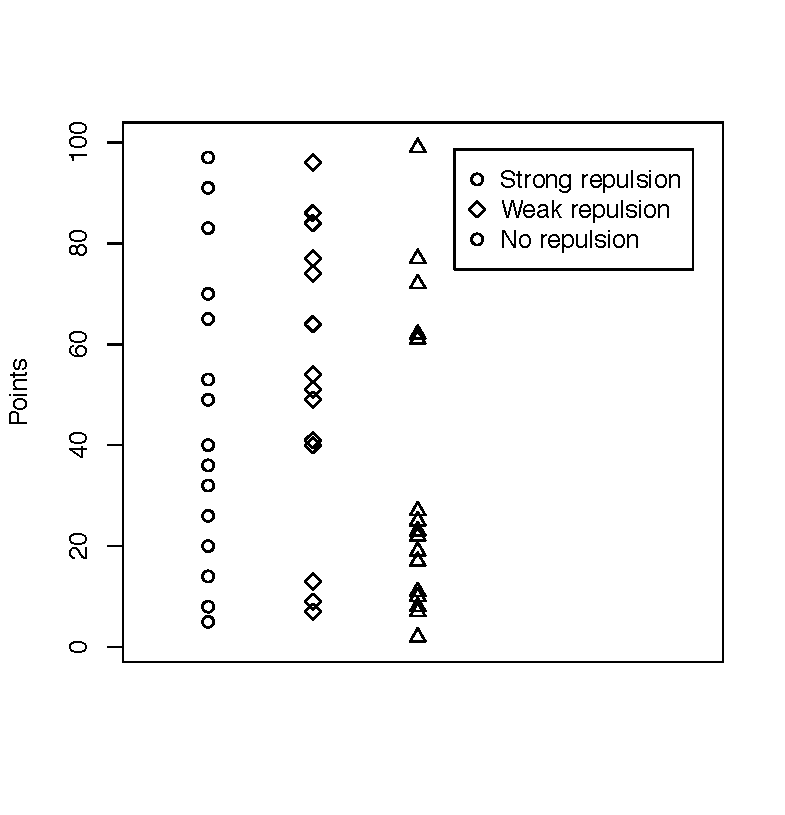
\includegraphics[width=0.60\textwidth]{figures/comparison-different-DPPs-Poisson-4}
%	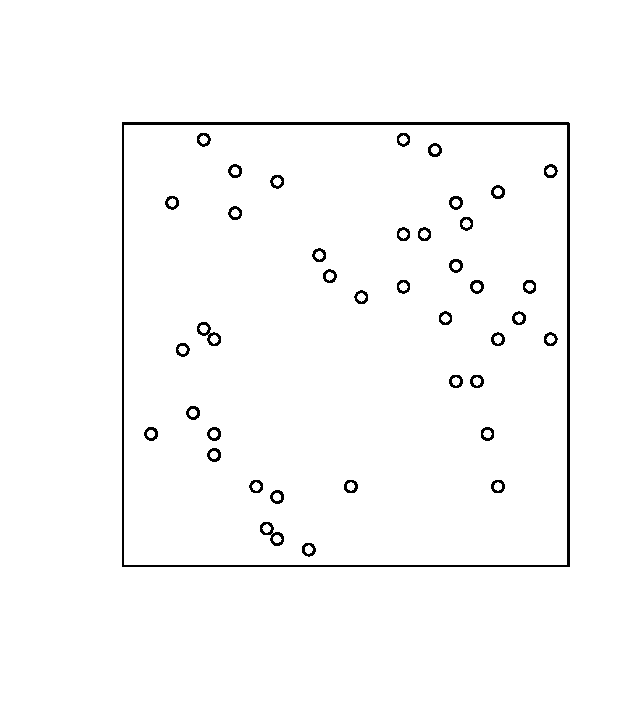
\includegraphics[width=0.49\textwidth]{Poisson-in-square}
%	\tag{1}
	\caption{Two DPPs with a different strength of repulsion on the left and a Poisson point process on a (discretised) line with same expected cardinality. The spatial repulsion of the DPPs is clearly visible.}
	\label{pointsonaline}
\end{figure}

We shall quickly discuss what influence the choice of \(f\) has on the strength of the repulsion of the DPP. %Indeed lets say we choose
%\[(\phi_i)_j\propto \exp\left( - \frac{(i-j)^2}{\sigma}\right) \quad \text{for } i, j\in\mathcal Y\]
%for some \(\sigma>0\). Then we obviously have 
For this we let the parameter \(\sigma\) tend to infinity and note
\[\phi_i \xlongrightarrow{\sigma\to\infty} \sqrt{N}\cdot \begin{pmatrix}
1\\ \vdots \\ 1
\end{pmatrix}\in\mathbb R^N. \]
Hence the similarity \(\phi_i^T\phi_j\) between item \(i\) and \(j\) will increase and therefore the negative correlation gets stronger as \(\sigma\) grows. Hence, the DPP will become increasingly repulsive if we increase the parameter \(\sigma\) which can be seen in Figure \ref{pointsonaline} where the first sample corresponds to the choice \(\sigma = 20\), the second one to \(\sigma = 5\) and the last one to a Poisson point process. On a more formal level one can argue that if one models the diversity feature vectors this way, we center Gaussian densities at the reference points and then associate an item \(i\) with how it looks seen from those reference points under this Gaussian density. If we increase the standard deviation \(\sigma\) of this density all items become increasingly similar in relation to the reference points. Similar considerations apply if \(f\) is not a normal density.%recent\todo{is this similar to kernel methods?}
% \todo{complete this and add picture!}

\subsubsection*{Binary sequences}

It is well known that a \(0-1\) sequence that is generated by a human will typically differ strongly from a randomly generated \(0-1\) sequence.\footnote{At least if the human is sufficiently unfamiliar with statistics.} For example the total amount of changes between zeros and ones is typically significantly higher in the human pseudorandom sequence. Also the length of the longest chain of zeros or ones will likely be significantly shorter (cf. \cite{ruschendorf2014mathematische}). Hence, the position of the ones tend to repell themselves since a human will typically think that a long chain of successive ones will be untypical for a random sequence and thus one could model these positions through a DPP.

We will consider \(0-1\) sequences of length 30 and therefore set \(\mathcal Y \coloneqq \left\{ 1, \dots, 30\right\}\) and define the DPP in the exact same way as above. Again, we choose \(f\) to be a normal density, but will choose the variance such that the repulsion is visible but not too strong and scale the qualities such that the expected cardinality is \(15\), since a human would probably aim to write down around \(15\) ones. In completely analogue fashion to the previous examples we define a Poisson point process with the same expected cardinality. This time we will represent the samples from the two point processes through a \(0-1\) sequence where a \(1\) at the \(i\)-th position indicates that item \(i\) was in the sample. We obtain the two following samples:
\begin{equation*}
\begin{split}
& 1 0 1 0 0 1 0 1 1 0 1 0 0 0 1 0 1 0 0 1 0 1 0 1 0 1 0 0 1 1 \\
& 1 1 1 1 1 1 1 0 1 0 1 0 0 0 0 1 1 0 1 0 0 0 1 1 0 1 0 0 1 1
\end{split}
\end{equation*}
Although the first sequence might actually look more random at first, this one is the one generated by the DPP and on second sight one realises that the positions of the ones are negatively correlated. Indeed in the first sequence the longest chain of zeros or ones is of length three, in the second one of length seven. The amount of changes between zero and one is \(22\) in the first sequence and only \(14\) in the second sequence.%\todo{comment on \(0-1\) sequences arising from random digit sequence}

Although the DPP presented above incorporates some of the properties one might expect from a \(0-1\) sequence created by a human, this process will not exactly be determinantal. However, it shall be noted that different \(0-1\) sequences studied in probability theory exhibit an exact determinantal structure. For example Borodin studied the sequence of descent positions in \cite{borodin2010adding}. To obtain those sequences one first samples a sequence of \(N+1\) independent digits \(\left\{ 0, 1, \dots, 9\right\}\). Then one marks the positions in \(\left\{ 1, \dots, N\right\}\) where the successor of the digit is strictly smaller than the current digit. The heuristical argument why those positions of descent repell themselves is that if \(k\) is not a point of descent, then the digit on the position \(k+1\) is likely to be big and hence likely to be a point of descent.

\subsubsection{Points in a square}

This time we want to built a DPP in a two dimensional square \([0,1]^2\) or at least a discrete approximation of it. This might be used to model positions of trees that repel themselves due to a competition for natural resources, positions of football players on the field or the positions people choose for a picnic in a park.

In order to do this we follow an approach similar to the case of the one dimensional DPPs. Hence, we set
\[\mathcal Y \coloneqq 99^{-1} \left\{ 0, \dots, 99\right\}^2 \]%\left\{ (i, j) \mid 39\cdot  \right\} \]
and obtain a \(100\times 100\) grid covering the unit square. We again choose \(\mathcal R \coloneqq \mathcal Y \) and \(f\) to be the normal density with mean \(0\) and variance \(\sigma>0\). Then we choose the similarity feature vectors to be 
\[(\phi_i)_j\propto f(\left\lVert i - j \right\rVert) \quad \text{for } i, j\in\mathcal Y.\]
where \(\left\lVert \cdot \right\rVert\) is the Euclidean norm. We propose constant qualities just like before and scale them and also the variance \(\sigma\) in such a way that we get a reasonable cardinality and also a notable repulsion of the DPP. %This is done by trial and error.
The resulting samples are depicted in Figure \ref{pointsinthesquare}.
\begin{figure}[h!]
	\centering
	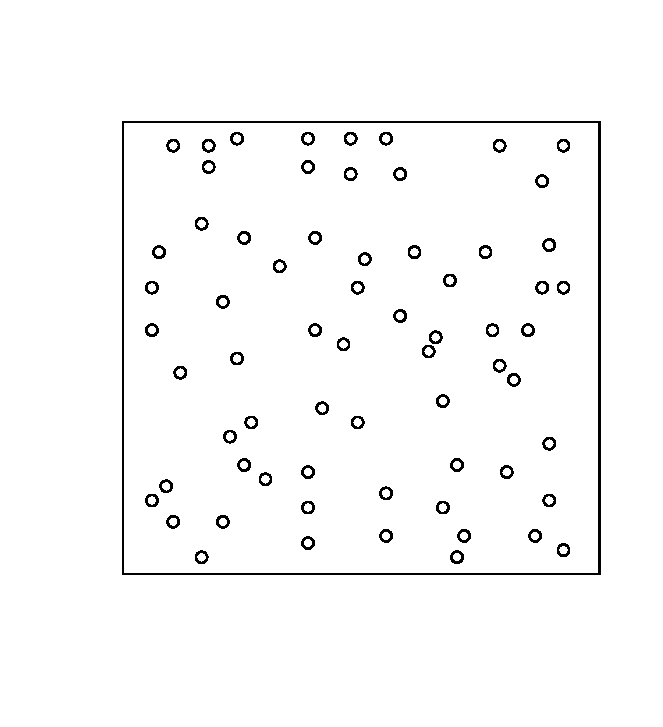
\includegraphics[width=0.444\textwidth]{figures/DPP-in-square-large-3}
	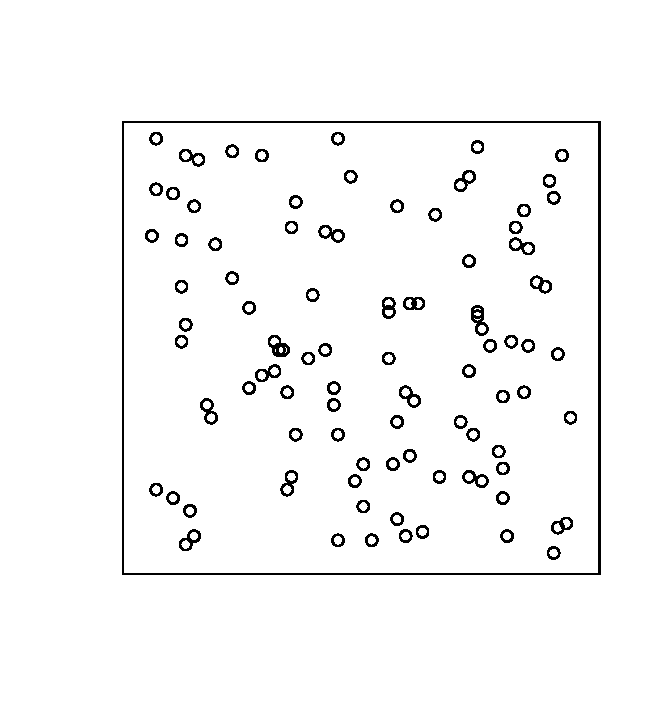
\includegraphics[width=0.44\textwidth]{figures/Poisson-in-square-large-2}
	\caption{A DPP (right) and a Poisson point process (left) on a \(100\times100\) grid in the unit square with the same expected cardinality. The -- in this case spatially -- repellent structure of the DPP is clearly visible.}
	\label{pointsinthesquare}
\end{figure}

It should be noted at this stage, that the simulation of the DPP can still be performed in relatively short time, even without making use the dual sampling or the random projections. In fact one sample could be produced on a six year old MacBook air with only one processor in about two minutes. This is actually quite astonishing given that the DPP is a discrete probability distribution over \(2^{10^4} \approx 10^{3000}\) elements. This is roughly the estimated number of elementary particles in the universe to the power of 35.

Assume now that we have some reason to believe that the qualities of the individual points on the grid are not equal. Maybe there might be a road just around the park and hence people prefer to sit in the middle of the park and we can implement this into our model by letting the qualities of the items decrease depending on their distance to the centre \(m \coloneqq(0.5, 0.5)\) of the grid. More precisely we choose
\[q_i\coloneqq a \cdot \exp\big(-b \left\lVert i - m \right\rVert\big) \]
where \(a, b>0\) are scaled such that the decrease of quality is visible but not too strong and that a reasonable cardinality of the DPP is obtained. The results for this can be seen in Figure \ref{pointsinthesquarelog}.
\begin{figure}[h!]
	\centering
	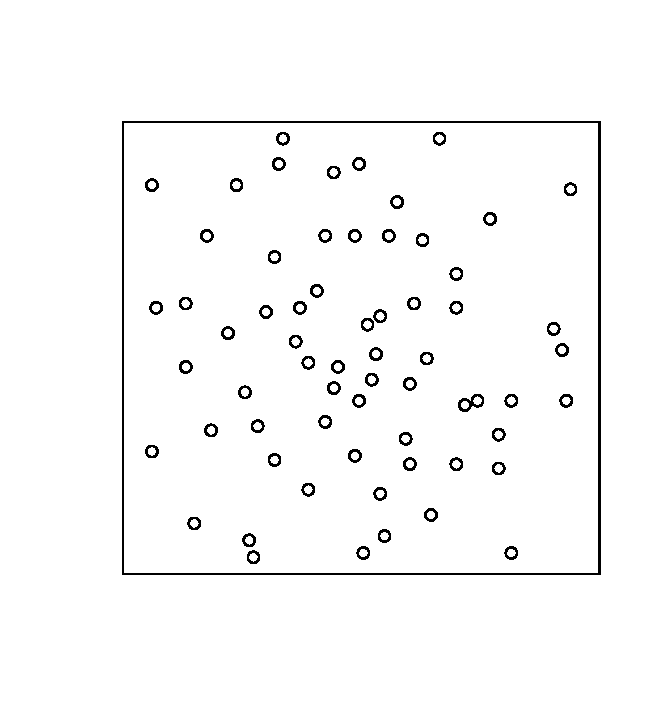
\includegraphics[width=0.60\textwidth]{figures/DPP-in-square-large-log-linear}
	\caption{A DPP on a \(100\times100\) grid in the unit square with decreasing quality towards the edges.}
	\label{pointsinthesquarelog}
\end{figure}

\clearpage
%one core \(1.8\si{Ghz}\) Intel i5 MacBook Air in around \(\si{s}\). 

%\section{Calculations}

%\begin{enumerate}
%\item Complement of DPPs
% \item Explain why every suitably definite matrix is a marginal kernel
%\item Expression of elementary probabilities
%\end{enumerate}

\chapter{Point estimators and parametric models}

%\section{What does learning mean and why is it interesting?}
%\todo{what is learning?}
%\todo{general overview over this chapter}
%\todo{explain bias and consistency}
% \section{Motivation for learning DPPs}

Parameter estimation is one of the central components of every theory of real world phenomena. In a nutshell one could split the process of the construction of a descriptive model into two parts. The first one being the selection of the model which is done by a scientist and the second being the determination of the constants that belong to the model.

To make this more clear we will consider one of the most famous advances in the natural sciences namely the law of universal gravitation that was discovered by Sir Isaac Newton\todo{cite}. More precisely Newton discovered that the gravitational force acting between two massive objects is given by
\[F = G\cdot \frac{m_1m_2}{r^2}\]
where \(m_1, m_2\) are the masses of the two objects, \(r\) is the distance of the centers of masses and \(G\) is the gravitational constant. This constant can not be deduced from the theory itself and needs to be estimated based on some empirical data.

If we want to describe, simulate and predict the occurence of diverse subsets we can take a similar approach and impose the model of a determinantal point process. % which would correspond to the first part
This will usually be an assumption that will not strictly hold, but will often lead to reasonable, sometimes even impressive results. We will not be concerned in a measure of how justifiable this model selection is, although this is a highly interesting question and there exist ways to deal with it\todo{cite paper about KL divergence}. Leaving that aside we are left with the second step, namely the estimation of the parameters of the model, which are in the case of a DPP over a set of cardinality \(N\) exactly \(N(N-1)/2\). Because of the rather large amount of parameters and also the complicated structure of the DPPs it will in practice only be possible to perform those estimations through the use of computational tools. The task of computer based parameter or density estimation is an important field in the discipline of \emph{machine learning} and thus we will sometimes speak of the parameters being learned instead of estimated. Actually the interest of parameter estimation for DPPs arose from the machine learning community at the beginning of this decade. However we will phrase things in a way that no prior knowledge in this field is required.

In this chapter we will be concerned in how we can make point estimates for either the marginal or the elementary kernels \(K\) and \(L\). Point estimators are the most basic type of estimators and consist of the suggestion of one possible parameter set, for example in the case of the gravitational constant 
\[6.674\cdot10^{-11}\si{N.kg^{-2}.m^2}. \]
This is in contrast to the Bayesian approach to parameter estimation that we will present in the next chapter where the philosophy is to estimate a distribution over all possible parameter sets that indicates how likely they are given some the empirical data. We will discuss two essentially different methods of point estimators, the first one provides a way to reconstruct a marginal kernel for the empirical marginal distributions at least in the case where the empirical distribution is essentially a DPP. The other type of methods are all maximum likelihood estimators in different variations. 

But before we can proceed we want to remind the reader of two desirable properties of point estimators. For this we will assume that we want to estimate the distribution of a random variable \(X\) from a parametric family of probability measures
\[\left\{ \mathbb P_\theta\mid \theta\in\Theta\right\}.\]
This means we want to estimate \(\theta\) out of a possible set of parameters \(\Theta\) such that \(X\) is distributed according to \(\mathbb P_\theta\) which we will based upon some data \(x_1, \dots, x_n\). Further we assume that those points are actually generated by \(\mathbb P_\theta\) for one \(\theta\in\Theta\) and denote the estimator by \(\hat\theta_n\). We call \emph{unbiased} if we have
\[\mathbb E[\hat\theta_n] = \theta\]
and \emph{consistent} if we have
\[\hat\theta_n\to\theta \quad \text{in probability}.\]

It shall be noted that although those properties are beneficial, they are not crucial for an estimator to be reasonable. First they both assume that the data generating process, i.e. the process one wants to describe actually follows one of the laws \(\mathbb P_\theta\) which will typically be not the case in real world examples. Further the asymptotic property of consistency is rather of theoretical nature since in practice it is not possible to create large sets of empirical data and certainly not infinitely large ones. 

%In practice this will be a rather large amount of parameters and therefore it will only be possible

\section{Kernel reconstruction of the empirical measures} %  via the Assymptotic reconstruction of the kernel}

%In this section we want to see how we can estimate the marginal kernel from an increasing number of observations \(\mathbf Y_1, \dots, \mathbf Y_n\subseteq \mathcal Y\) that are distributed according to \(\mathbb P\). For this we will sketch the procedure in \cite{urschel2017learning}. 
Now we will display the first way how one can estimate the marginal kernel \(K\) of a DPP based on some samples drawn from it.

\begin{emp}[Setting]
Let \(\mathcal Y\) be a finite set of cardinality \(N\) and let \(K\in\mathbb R^{\mathcal Y\times\mathcal Y}_{\text{sym}}\) satisfy \(0\le K\le I\). Let further \(\mathbf Y_1, \mathbf Y_2, \dots\) be distributed according to the DPP with marginal kernel \(K\).
\end{emp}

In order to perform an approximate reconstruction of the marginal kernel we will need to consider the \emph{empirical measure} % \(\hat{\mathbb P}_n\) be 
\[\hat{\mathbb P}_n \coloneqq \frac1n\sum_{i=1}^n\delta_{\mathbf Y_i}.\]
% We can identify the probability measures on a finite set, in our case \(2^{\mathcal Y}\), with the probability simplex
% \[\left\{ x\in\mathbb R^{2^{\mathcal Y}} \;\Big\lvert\; x_A \in[0, 1] \text{ for all } A\in 2^{\mathcal Y} \text{ and } \sum_{A\in 2^{\mathcal Y}} x_A = 1 \right\}.\]
The interest in \(\hat{\mathbb P}_n\) lies in the fact that they quite natural estimates for the actual underlying distribution. 
% It is well known that \(\hat{\mathbb P}_n\) 
More precisely they are {unbiased estimators} for \(\mathbb P\), i.e. they agree in expectation with \(\mathbb P\). This can be seen by evaluating it at \(A\subseteq \mathcal Y\)
\[\mathbb E_{\mathbb P}\big[\hat{\mathbb P}_n(A)\big] =\frac1n \sum_{i = 1}^n \mathbb E_{\mathbb P}\big[\delta_{\mathbf Y_i}(A)\big] =  \mathbb P(A).\]
And even stronger by the strong law of large numbers they converge to \(\mathbb P\) almost surely if the sequence \((\mathbf Y_k)_{k\in\mathbb N}\) of observations is independent. This can be seen by identifying the probability measures on \(2^{\mathcal Y}\) with the probability simplex
\[\left\{ \mu\in\mathbb R^{2^{\mathcal Y}} \;\Big\lvert\; \mu_A\in[0, 1] \text{ for all } A\subseteq\mathcal Y \text{ and } \sum_{A\subseteq\mathcal Y}\mu_A = 1 \right\}\]
and using the strong law of large numbers in \(\mathbb R^{2^{\mathcal Y}}\).

Therefore the empirical measures are reasonable approximations of the actual probability distribution. Assume now for one moment that the empirical measures \(\hat{\mathbb P}_n\) are also determinantal point processes with marginal kernel \(\hat K_n\), then \(\hat K_n\) would be a quite intuitive estimate for the actual marginal kernel \(K\). Thus we are interested in the question whether we can reconstruct the kernel marginal of a DPP if we know the DPP itself. Since the marginal density of a DPP corresponds to the principal minors of the marginal kernel, we first investigate whether we can reconstruct a matrix from its principle minors. For the answer to this problem we follow the main ideas presented in \cite{urschel2017learning} and \cite{rising2015efficient} although we modify their arguments to make them shorter and hopefully more accessible.% \todo{say something about stability?}


%Therefore we can consistently %\todo{explain consistency}{ } 
%estimate all principal minors of \(K\), since
%\[\hat{\mathbb P}_n(A\subseteq \mathbf Y) \xlongrightarrow{n\to\infty} \mathbb P(A\subseteq\mathbf Y) = \det(K_A) \quad \text{almost surely}.\]


%Assume that \(\hat{\mathbb P}_n\) is a DPP with marginal kernel \(\hat K_n\), then \(\hat K_n\) would be a quite natural estimate for the actual marginal kernel \(K\).
%To make this approach rigorous we have to convince ourselves that the empirical measure are in fact DPPs and that a marginal kernel can be reconstructed from the DPP.

%it is natural to ask whether we can reconstruct the kernel 



% Thus the question naturally arrises whether we can reconstruct the kernel \(K\) from the knowledge of all of its principal minors, which we will address in the following.

%\subsubsection*{The principal minor assignment problem}\todo{phrase it very clearly}
%\todo{define principle minors?}
\begin{emp}[The principal minor assignment problem]
Let \(K\in\mathbb R^{N\times N}\) be a symmetric matrix. We want to investigate whether \(K\) uniquely specified by its principle minors
\[\Delta_S \coloneqq \det(K_S) \quad \text{where } S\subseteq\left\{ 1, \dots, N\right\}.\]
We call this the \emph{symmetric principal minor assignment problem} and it will turn out that the matrix \(K\) can be reconstructed up to an equivalence relation.
\end{emp}

%The reconstruction of a symmetric matrix from all its principal minors is known as the \emph{principal minor assignment problem} and we aim to prove in this section that this is possible -- at least up to an equivalence relation. 
Before we present the general procedure we want to see how this would work in the case of a symmetric \(3\times3\) matrix \(K = (K_{ij})_{1\le i, j\le 3}\). First we note that we can regain the diagonal elements as the determinant of the \(1\times1\) principal minors
\[\det(K_{\left\{ i\right\}}) = K_{ii} \quad \text{for } i = 1, 2, 3.\]
Further the squares of the off diagonal are determined by the \(2\times2\) principal minors since
\[\det(K_{\left\{ i, j\right\}}) = K_{ii}K_{jj} - K_{ij}^2 \quad \text{for }i, j = 1, 2, 3.\]
Therefore we only need to reconstruct the signs off diagonal entries. To do this, we consider the determinant of the matrix itself
\begin{equation}\label{thrtimthr}
\det(K) = K_{11}K_{22}K_{33} + 2K_{12}K_{13}K_{23} - K_{11}K_{23}^2 - K_{22}K_{13}^2 - K_{33}K_{12}^2.
\end{equation}
Rearranging this yields
\[K_{12}K_{13}K_{23} = \frac12\left( \det(K) + K_{11}K_{23}^2 + K_{22}K_{13}^2 + K_{33}K_{12}^2 - K_{11}K_{22}K_{33}\right).\]
Since we know all of the expressions on the right side, we can determine the sign of the product on the left side. Now we assign the signs of the off diagonal elements in such a way, that the above equation holds. More precisely if the product is negative, we assign a minus to one or all three elements, if it is positive, then we assign a minus to none or two elements. If the product is zero, every configuration of signs satisfy the desired property. It is now straight forward to check that this assignment actually leads to the desired principle minors.
% \todo{explain this.}

One main part in the general procedure will be to obtain a generalisation of the formula \eqref{thrtimthr} for larger principle minors that will allow the reconstruction of the signs. For this we will need the following graph theoretical concepts.
%In order to generalise the procedure above to larger matrices we will need some elementary concepts from graph theory.


\begin{emp}[Notions from graph theory]
Let \(G = (V, E)\) be a finite graph, i.e. \(V\) is a finite set, called the \emph{vertex set} and \(E\) consists of subsets of \(V\) with two elements, the \emph{edges}. Sometimes we will be sloppy in notation and not distinguish between the graph and the edge set. We will need the following notions:
\begin{enumerate}
\item \emph{Degree:} For a vertex \(v\in V\) the \emph{degree} is the number of edges that contains \(v\). 
\item \emph{Subgraph:} A graph \(\tilde G = (\tilde V, \tilde E)\) is called a \emph{subgraph} of \(G\) if \(\tilde V\subseteq V\) and \(\tilde E\subseteq E\).
\item \emph{Induced graph:} For a subset \(S\subseteq V\) of vertices the \emph{induced graph} \(G(S) = (S, E(S))\) is formed of all edges \(e\in E\) of \(G\) that are subsets of \(S\).
\item \emph{Path:} A \emph{path} in \(G\) is a sequence \(v_0v_1\cdots v_k\) of vertices such that \(\left\{ v_{i-1}, v_{i}\right\}\in E\) for all \(i = 1, \dots, k\).
\item \emph{Connected graph:} A graph is called \emph{connected} if for every pair of vertices \(v, w\in V\) there is a path from \(v\) to \(w\).
%, i.e. there is a sequence \(\left\{ v, v_1\right\}, \left\{ v_1, v_2\right\}, \dots, \left\{ v_{k-1}, v_k\right\}, \left\{ v_k, w\right\}\) of edges.
\item \emph{Cycle:} A \emph{cycle} \(C\) is a connected subgraph such that every vertex has even degree in \(C\). 
\item \emph{Cycle space:} Each cycle \(C\) can be identified with a vector \(x = x(C)\in\mathbb F_2^{E}\) such that
\[x_e\coloneqq \begin{cases} 1 \quad & \text{if } e\in C \\ 0 \quad & \text{if } e\notin C\end{cases}\]
indicates whether the edge \(e\in E\) belongs to the cycle \(C\). The \emph{cycle space} \(\mathcal C\) is the span of \(\left\{ x(C)\mid C\text{ is a cycle}\right\}\) in \(\mathbb F_2^{E}\). Note that the sum of two cycles in the cycle space corresponds to the symmetric difference of the edges.
%\item \emph{Simple cycle:} A cycle is called \emph{simple} if every vertex of \(C\) has even degree in \(C\).
%\item \emph{Cycle basis:} A basis of the cycle space is called \emph{cycle basis} if it consists of simple cycles.
\item \emph{Chordless cycle:} A cycle \(C\) is called \emph{chordless} if two verteces \(v, w\in C\) form an edge in \(G\) if and only they form an edge in \(C\). This is equivalent to the statement that \(C\) is an induced subgraph that is a cycle.
\item \emph{Cycle sparsity:} The cycle sparsity is the minimal number \(l\) such that a basis of the cycle space consisting of chordless simple cycles exists. Such a basis is called \emph{shortest maximal cycle basis} or short \emph{SMCB}. If the cycle space is trivial we define the cycle sparsity to be \(2\).
\item \emph{Pairings:} Let \(S\subseteq V\) be a set of of vertices. Then a \emph{pairing} \(P\) of \(S\) is a subset of edges of \(G(S)\) such that two different edges of \(P\) are disjoint. The vertices contained in the edges of \(P\) are denoted by \(V(P)\) and the set of all pairings by \(\mathcal P(S)\).
\end{enumerate}
\end{emp}\todo{add pictures and explanations?}

It is highly recommended to draw some examples in order to get more familiar with the definitions above. To see that the above definition of the cycle sparsity is well defined, we have need to show that shortest maximal cycle basis exist. This might be well known to people that are familiar with graph theory, but we will present an elementary proof here. The first part of the statement, namely the existence of cycle basis consisting of simple cycles is known as Veblen�s theorem and can be found in its original form in \cite{10.2307/1967604}, however we will rather follow the approach in \cite{bondy2011graph}.
%It shall be noted, that the proof -- and also the definitions above -- becomes quite a lot more intuitive by drawing the according cycles in order to understand how the respective decompositions of cycles work.

\begin{prop}[Existence of SMCBs]
There always exists a basis \(\left\{ x(C_1), \dots, x(C_k)\right\}\) of the cycle space where \(C_1, \dots, C_k\) are chordless simple cycles.
\end{prop}
\begin{proof}
First we prove that the set of simple cycles generates the whole cycle space which we can then improve to show that the simple chordless cycles already generate the cycle space. A shortest maximal cycle basis is then attained by successively dropping simple chordless cycles.

We show that every cycle \(x(C)\) can be written as the sum of simple cycles \(x(C_1), \dots, x(C_k)\) where \(C_i\subseteq C\). This is equivalent to the statement that the edges of every cycle are the disjoint union of the edges of simple cycles. Take now a maximal non intersecting path \(v_0v_1\cdots v_k\).
\begin{figure}[h!]\label{makesimple}
	\centering
\begin{tikzpicture}%[shorten >=1pt,->]

  \tikzstyle{vertex}=[draw,circle,minimum size=17pt,inner sep=0pt]

  \foreach \name/\angle/\text in {A-1/234/1, A-2/162/2, 
                                  A-3/90/3, A-4/18/4, A-5/-54/5}
    \node[vertex,xshift=5cm,yshift=.5cm] (\name) at (\angle:1.3cm) {\(\text\)};
    
  \foreach \name/\angle/\text in {B-1/234/1, B-2/162/2, 
                                  B-3/90/3, B-4/18/4, B-5/-54/5}
    \node[vertex,xshift=9cm,yshift=.5cm] (\name) at (\angle:1.3cm) {\(\text\)};

  \foreach \from/\to in {1/2,2/3,3/4,4/5,5/1,1/3,5/2}
    \draw (A-\from) -- (A-\to);

\foreach \from/\to in {1/2,2/5,5/4,4/3}
\draw (B-\from) -- (B-\to);
\foreach \from/\to in {1/3,2/3,1/5}
\draw[dashed] (B-\from) -- (B-\to);
\end{tikzpicture}
\caption{Illustration of the search for a simple cycle in a graph with degrees greater than two. Once a maximal non intersecting path like \(12543\) is selected, every continuation of the path -- in this case 2 or 1 -- is already present in the path and therefore induces a simple cycle.}
\end{figure}
Since \(v_k\) has degree at least \(2\), there is an edge \(\left\{ v_k, v_{k+1}\right\}\) such that \(v_{k+1}\ne v_{k-1}\). Since the path is maximal, \(v_{k+1}\) has to agree with one a vertex \(v_i\in\left\{ v_0, \dots, v_{k-2}\right\}\), because otherwise we could add \(v_{k+1}\) to the path which is a contradiction to the maximality. Now \(v_iv_{i+1}\cdots v_kv_i\) corresponds to a simple cycle \(C_1\) and \(C_2\coloneqq C\setminus C_1\) is again a cycle. Thus we can write \(C\) as the disjoint union \(C = C_1\cup C_2\) where \(C_1\) is a simple cycle. By repeating this procedure we get the desired expression for \(C\) in terms of simple cycles.

To prove that already the simple chordless cycles generate the cycle space we have to prove that we can write every simple cycle \(x(C)\) as a sum of simple chordless cycles \(x(C_1), \dots, x(C_k)\). Let \(\left\{ \left\{ v_0, v_1\right\}, \dots, \left\{ v_k, v_0\right\}\right\}\) be the edge set of \(C\) and assume that \(C\) is not chordless like in Figure \ref{makechordless}, otherwise the statement would be trivial.
\begin{figure}[h!]\label{makechordless}
	\centering
\begin{tikzpicture}%[shorten >=1pt,->]

  \tikzstyle{vertex}=[draw,circle,minimum size=17pt,inner sep=0pt]

  \foreach \name/\angle/\text in {A-1/234/1, A-2/162/2, 
                                  A-3/90/3, A-4/18/4, A-5/-54/5}
    \node[vertex,xshift=5cm,yshift=.5cm] (\name) at (\angle:1.3cm) {\(\text\)};
    
  \foreach \name/\angle/\text in {B-1/234/1, B-2/162/2, 
                                  B-3/90/3, B-4/18/4, B-5/-54/5}
    \node[vertex,xshift=9cm,yshift=.5cm] (\name) at (\angle:1.3cm) {\(\text\)};

  \foreach \name/\angle/\text in {C-1/234/1, C-2/162/2, 
                                  C-3/90/3, C-4/18/4, C-5/-54/5}
    \node[vertex,xshift=13cm,yshift=.5cm] (\name) at (\angle:1.3cm) {\(\text\)};

  \foreach \from/\to in {1/2,2/3,3/4,4/5,5/1}
    \draw (A-\from) -- (A-\to);
\draw[dashed] (A-1) -- (A-3);

\foreach \from/\to in {1/2,2/3,3/1}
\draw (B-\from) -- (B-\to);
\foreach \from/\to in {3/4,4/5,5/1}
\draw[dashed] (B-\from) -- (B-\to);

\foreach \from/\to in {1/2,2/3}
\draw[dashed] (C-\from) -- (C-\to);
\foreach \from/\to in {1/3,3/4,4/5,5/1}
\draw (C-\from) -- (C-\to);
\end{tikzpicture}
\caption{The simple cycle \(123451\) on the left is not chordless but the symmetric difference of the two simple chordless cycles \(1231\) and \(13451\) on the right.}
\end{figure}
 Thus there is are indices \(1\le i<j-1\le k-1\) such that \(\left\{ v_i, v_j\right\}\in E\). Let now \(C_1\) and \(C_2\) be the two cycles associated with the paths
\[v_0v_1 \cdots v_iv_jv_{j+1}\cdots v_kv_0\quad \text{and } v_iv_{i+1}\cdots v_{j-1}v_jv_i.\]
Then we have \(x(C) = x(C_1) + x(C_2)\). By iterating this procedure as long as the cycles are not chordless the desired decomposition can be achieved in finitely many steps.

%Since we have defined the cycle space as the span of all vectors \(x(C)\) where \(C\) is a cycle, it suffices to show that every cycle \(C\) admits a decomposition
%\[x(C) = x(C_1)+\dots+x(C_m)\]
%where \(C_1, \dots, C_m\) are chordless cycles. If \(C\) is already chordless, then we are done, so we can assume that the vertices of \(C\) are \(\left\{ v_1, \dots, v_M\right\}\) with\todo{finish this proof!}
\end{proof}%\todo{cite the theorem with its actual name}

\begin{defi}[Determinantal equivalence]
Two symmetric matrices \(A, B\in\mathbb R^{N\times N}\) are called \emph{determinantally equivalent} if the have the same principal minors and we write \(A\sim B\).
\end{defi}

It is obvious that we can only hope to reconstruct a symmetric matrix up to determinantal equivalence. However this would be satisfactory, because determinantally equivalent matrices are exactly those that give rise to the same DPP. Let us in the following denote the principal minor \(\det(K_S)\) by \(\Delta_S\) for \(S\subseteq\left\{ 1, \dots, N\right\}\). To come back to our original problem, we notice that the principal minors up to size two immediately determine the diagonal and the absolute values of the off diagonal of \(K\) since we have
\begin{equation*}\label{e3.0}
K_{ii} = \Delta_{\left\{ i\right\}} \quad \text{and } K_{ij}^2 = K_{ii}K_{jj} - \Delta_{\left\{ i, j\right\}}.
\end{equation*}
Thus it only remains to regain the signs \(\operatorname{sgn}(K_{ij})\) of the off diagonal entries. For this we use the following object.

\begin{emp}[The adjacency graph and sign function]
The adjacency graph \(G_K = (V_K, E_K)\) associated with \(K\) consists of the vertex set \(\left\{ 1, \dots, N\right\}\) and \(\left\{ i, j\right\}\) form an edge if and only if \(K_{ij}\ne0\). Further we introduce some \emph{weights} on the edges. This means we consider a mapping \(w\colon E_K\to\mathbb R\) and we set
\[w_{ij} \coloneqq w(\left\{ i, j\right\}) \coloneqq \operatorname{sgn}(K_{ij})\]
where we call \(w_{ij}\) the weight of the edge \(\left\{ i, j\right\}\). This graph together with the weights determines the signs of the off diagonal elements, so we are interested in reconstruction the weights from the principal minors.
Finally we define the sign of a cycle and for a cycle \(C = (S, \tilde E)\) we set \(\operatorname{sgn}(C) \coloneqq\prod_{e\in \tilde E}w_e\). It will become important later to consider this sign function on the cycle space and thus we note that this definition corresponds to
\[\operatorname{sgn}(x(C)) \coloneqq \prod_{e\in E} w_e^{x(C)_e}.\]
Note that this is a group homomorphism from the cycle space \(\mathcal C\) to \(\left\{ \pm1\right\}\) and therefore it is uniquely determined by its value on a generator, for example on a shortest maximal cycle basis.
\end{emp}

\begin{prop}[Principal minors of simple chordless cycles]
Let \(C = (S, E(S))\) be a simple and chordless cycle. Then the principal minor of \(K\) with respect to \(S\) is given by
\begin{equation}\label{pmcl}
\Delta_S = \sum_{P\in\mathcal P(S)} (-1)^{\left\lvert P \right\rvert}\cdot \!\!\!\prod_{\left\{ i, j\right\}\in P}\! K_{ij}^2 \cdot\!\!\prod_{i\notin V(P)}\! K_{ii} + 2\cdot (-1)^{\left\lvert S \right\rvert + 1}\cdot\!\!\!\!\!\!\prod_{\left\{ i, j\right\} \in E(S)} \!K_{ij}.
\end{equation}
\end{prop}
\begin{proof}
Let \(k\coloneqq \left\lvert S \right\rvert\). Then by Leibniz formula we have
\[\Delta_S = \sum_{\sigma\in S_k} \operatorname{sgn}(\sigma) \prod_{i\in S} K_{i\sigma(i)} \]
where \(S_k\) is the set of permutations of \(S\). Note that since the cycle is chordless, the product is only non trivial if \(\left\{ i, \sigma(i)\right\}\in E(S)\) for all \(i\in S\). Since \(C\) is a simple cycle, those permutations consist exactly of the pairing of \(S\) or the two shifts of the set \(S\) along the cycle in both directions. Those correspond exactly to the summands in \eqref{pmcl}.

To see this, we fix a permutation \(\sigma\) such that \(\left\{ i, \sigma(i)\right\}\) always forms an edge in \((S, E(S))\). We note that every vertex \(i\in S\) has two possible images which are exactly the endpoint of its two edges, c.f. Figure \ref{pm}.
\begin{figure}[h!]\label{pm}
	\centering
\begin{tikzpicture}
  \tikzstyle{vertex}=[draw,circle,minimum size=17pt,inner sep=0pt]

  \foreach \name/\angle/\text in {A-1/234/1, A-2/162/2, 
                                  A-3/90/3, A-4/18/4, A-5/-54/5}
    \node[vertex,xshift=5cm,yshift=.5cm] (\name) at (\angle:1.3cm) {\(\text\)};
    
 \foreach \name/\angle/\text in {B-1/234/1, B-2/162/2, 
                                  B-3/90/3, B-4/18/4, B-5/-54/5}
    \node[vertex,xshift=9cm,yshift=.5cm] (\name) at (\angle:1.3cm) {\(\text\)};

  \foreach \from/\to in {1/2,2/3,3/4,4/5,5/1}
    \draw (A-\from) -- (A-\to);
\draw[->] (A-5) to [out=50,in=-86] (A-4);
\draw[->] (A-4) to [out=-130,in=94] (A-5);
\draw[->] (A-3) to [out=194,in=58] (A-2);
\draw[->] (A-2) to [out=14,in=238] (A-3);

  \foreach \from/\to in {1/2,2/3,3/4,4/5,5/1}
    \draw (B-\from) -- (B-\to);
\foreach \to/\from in {1/2,2/3,3/4,4/5,5/1}
\draw[->] (B-\from) to [out={50 - \from * 72},in={- 86 - \from * 72}] (B-\to);
\end{tikzpicture}
\caption{An easy example for the two kinds of permutations of a chordless simple cycle that maps vertices to neighbors.}
\end{figure}
Lets assume it is mapped to \(j\in S\), then \(j\) has again two possible images under \(\sigma\) namely \(i\) and a second vertex \(k\in\mathcal Y\). If \(j\mapsto i\), no other vertex can be mapped to \(i\) or \(j\), however some other items can be swapped in the same way. The permutations of this form correspond exactly to the pairings of \(S\) and are represented in the first sum in \eqref{pmcl}. If however \(j\) is not mapped back to \(i\) but rather to its other neighbor \(k\), then \(k\) can�t get mapped back to \(j\) since \(\sigma\) is injective. Thus it has to be mapped to its other neighbor \(l\in\mathcal Y\). Through a repetition of this argument shows that this induces until \(i\) is reached again. Since the cycle is simple this path exhausts the entire cycle. The factor \(2\) is due to the fact that this shift of the indices can be done into either direction.
%A repetition of this argument shows that this chain of mappings has to continue until \(i\) is reached again. Since the cycle is chordless 
\end{proof}

\begin{prop}[Sign determines principals minors]
The knowledge of all principal minors up to size two and the sign function
\[\operatorname{sgn}\colon\mathcal C\to\left\{ \pm1\right\}\]
completely determines all principal minors of \(K\).
\end{prop}
\begin{proof}
Let \(S\subseteq\left\{ 1, \dots, N\right\}\) be arbitrary. We will again work with the expression \eqref{pmcl} of the principle minor \(\Delta_S\) and fix one permutation \(\sigma\). We can assume without loss of generality that \(\left\{ i, \sigma(i)\right\}\in E_K\) because the product it trivial otherwise. Since we know the absolute values of the off diagonal elements and the diagonal elements from the principle minors up to size two, it suffices to express the sign
\begin{equation}\label{e3.2}
\prod_{i\in S} \operatorname{sgn}(K_{i\sigma(i)})
\end{equation}
of the product through the sign function. For this we %fix one permutation \(\sigma\) and 
write \(\sigma\) as the product of disjoint cycles
\begin{equation}\label{e3.3}
\sigma = \sigma_1\circ \dots \circ \sigma_m
\end{equation}
where \(\sigma_k\colon D_k\to D_k\) for \(k = 1, \dots, m\) and the domains \(D_k\) are pairwise disjoint. The sign \eqref{e3.2} can be written as the product of
\[\prod_{i\in D_k} \operatorname{sgn}(K_{i\sigma_k(i)})\]
so it suffices to give expressions for those. Note that we could assume \(\left\{ i, \sigma_k(i)\right\}\in E_K\) and therefore \(C_k = (D_k, E_k)\) with
\[E_k = \left\{ \left\{ i, \sigma_k(i)\right\} \mid i\in D_k\right\}\]
is a cycle and therefore \eqref{e3.3} is equal to \(\operatorname{sgn}(C_k)\).
\end{proof}

\begin{theo}%[�]
Let \(K\in\mathbb R^{N\times N}\) be a symmetric matrix and \(l\) be the sparsity of its adjacency graph. Then the principal minors up to size \(l\) uniquely determine all principal minors of \(K\) and therefore the matrix \(K\) up to determinantal equivalence.
\end{theo}
\begin{proof}
In the light of the previous proposition it suffices to show that the sign function is uniquely specified by the principle minors up to size \(l\). Recall that the sign function is determined by its values on a shortest maximal cycle basis, which consists by definition of simple chordless cycles of length at most \(l\). However under the knowledge of the diagonal elements and the absolute values of the off diagonal ones, the sign of those simple chordless cycle is uniquely determined by the principle minors up to size \(l\) using the euqality \eqref{pmcl} .
\end{proof}
%\begin{rem}
%One can even show that this result is optimal in the sense that if one only has access to the principle minors up to size \(l-1\), then the equivalence class is not uniquely determined. See \cite{urschel2017learning} for details on this.\todo{can one also see this optimality from my proof?} \todo{comment on algorithms}
%\end{rem}
\begin{rem}
One can even show that this result is optimal in the sense that if one only has access to the principle minors up to size \(l-1\), then the equivalence class is not uniquely determined. To see this, we note that the sign function is not uniquely specified through the principle minors up to size \(l-1\) and thus there is more than one extension of the sign function onto the shortest maximal cycle basis. The equation \eqref{pmcl} shows that those different extensions give rise to different principle minors.
%See \cite{urschel2017learning} for details on this.\todo{can one also see this optimality from my proof?} \todo{comment on algorithms}
\end{rem}

\begin{emp}[Construction of the equivalence class]\label{cec}
We have shown that the determinantal equivalence class of a symmetric matrix is uniquely specified by its principle minors up to size \(l\). Now we want to investigate how this equivalence class can be computed and we will see that we can reduce this task to the solution of a system of linear equations over the finite field \(\mathbb F_2\).

Let us assume that we have knowledge of the principle minors \(\Delta_S\) for every \(S\subseteq\left\{ 1, \dots, N\right\}\) with size at most \(l\) and we want to construct a matrix \(\tilde K\) that is determinantally equivalent to \(K\). We have seen that we only need to reconstruct the signs of the off diagonal entries of \(K\) which is equivalent to reconstructing the edge weight \(w_{ij}\). To do this fix a shortest maximal cycle basis \(\left\{ C_1, \dots, C_m\right\}\) with vertex sets \(S_1, \dots, S_m\). Let us now rewrite \eqref{pmcl} in the form
\[H_k\coloneqq \Delta_{C_k} - \!\! \sum_{P\in\mathcal P(C_k)} (-1)^{\left\lvert P \right\rvert}\cdot \!\!\!\prod_{\left\{ i, j\right\}\in P}\! K_{ij}^2 \cdot\!\!\prod_{i\notin V(P)}\! K_{ii} = 2 \cdot (-1)^{\left\lvert C_k \right\rvert + 1} \operatorname{sgn}(C_k)\cdot\!\!\!\! \prod_{\left\{ i, j\right\}\in C_k}\left\lvert K_{ij} \right\rvert. \]
Given the principle minors, we can determine the value on the right side and taking the sign on both sides yields
\[ (-1)^{\left\lvert C_k \right\rvert + 1} \cdot \operatorname{sgn}(H_k) = \operatorname{sgn}(C_k) = \prod_{\left\{ i, j\right\}\in E(S_k)} w_{ij} \]
which we seek to solve for \(w\). However this multiplicative equation is hard to solve and therefore we use the canonical group isomorphism \(\phi\) between \(\left\{ \pm 1\right\}\) and \(\left\{ 0, 1\right\}\) to turn it into a linear equation. Setting \(x_{ij}\coloneqq \phi(w_{ij})\) we get that the condition above is equivalent to
\begin{equation*}
b_k\coloneqq \phi( \operatorname{sgn}(H_k)) + \lvert \hat S_k \rvert + 1 = \sum_{\left\{ i, j\right\}\in E(S_k)} x_{ij} = (Ax)_k \quad \text{in } \mathbb F_2
\end{equation*}
where \(A\) is the matrix with the rows \(x(C_k)^T\). Now we can fix any such solution \(x %= \phi(w)
\in\mathbb F_2^{E}\) of
\begin{equation}\label{linEqu}
Ax = b
\end{equation}
and we know that at least one exists, namely the one given by \(x_{ij} = \phi(\operatorname{sgn}(K_{ij}))\). %In the light of \eqref{e3.0} i
Let now \(w_{ij}\coloneqq x_{ij}\), then it is straight forward to see that \(\tilde K\) defined through
\[\tilde K_{ii} \coloneq\Delta_{\left\{ i\right\}} \quad\text{and } \tilde K_{ij} = w_{ij} \cdot \sqrt{\tilde K_{ii}\tilde K_{jj} - \Delta_{\left\{ i, j\right\}}} \]
is determinantally equivalent to \(K\).
%More precisely we seek to find weight \(w_{ij}\) such that \eqref{pmcl} holds. This is the case if and only if
\end{emp}

It shall be noted that there are algorithms with much better computational performance for the construction of the determinantal equivalence class. For some examples of efficient algorithms we refer to \cite{urschel2017learning} and \cite{rising2015efficient}.

%This is known as the \emph{principal minor assignment problem} and has been studied extensively (cf. \cite{griffin2006principal} and \cite{urschel2017learning}) and an computationally efficient algorithm has been proposed for the problem in \cite{rising2015efficient}. It is in fact possible to retain the matrix from its principal minors up to an equivalence relation which identifies matrices with each other, that have the same principal minors. Obviously this is sufficent for the task of learning a DPP, because those matrices are exactly those who give rise to the same point process. To see roughly how this reconstruction works we note that the diagonal is given by
%\[K_{ii} = \det(K_{\left\{ i\right\}})\]
%and the absolute value of the off diagonal can be obtained through
%\[K_{ij}^2 = K_{ii} K_{ii} - \det\big(K_{\left\{ i,j\right\}}\big). \]
%The reconstruction of the signs of the entries \(K_{ij}\) turns out to be the main difficulty, but this can be done analysing the cycles of the adjacency graph \(G_K\) corresponding to \(K\).%\todo{see whether this proof can be done in a simplified way without considering the sparsity \(l\)}
% The adjacency graph has \(\mathcal Y\) as its vertex set and the set of edges consists of the pairs \(\left\{ i,j\right\}\) such that \(K_{ij}\ne0\). The reconstruction now relies on the analysis of the cycles of this graph and it has been shown, that one only needs to know all the principal minors up to the order of the cycle sparsity of \(G_K\) (cf. \cite{urschel2017learning}). Following this method it is possible to compute estimators \(\hat K_n\) of \(K\) in polynomial time and give a bound on the speed of convergence in some suitable metric.\todo{state and assymptotic the result}

% In completely analogue fashion one can learn the elementary kernel \(L\).
% and those estimations can be used to sample from a DPP that was observed. This procedure might be sufficient in some scenarios, but this approach lacks the ability to extrapolate the knowledge one has of specific DPPs onto some new, unobserved DPPs which is exactly the point that would distinguish the procedure from classical statistics and would allow for far more interesting applications. To achieve this, we introduce the notion of conditional DPPs in the following section which are customised to describe families of DPPs with kernels that are in some way similar.#

%\subsubsection*{Definition of the estimator}


So far we have seen that the principle minors determine a symmetric matrix up to determinantal equivalence. However the empirical marginal densities do not in general need to be the principle minors of any symmetric matrix, in other words the empirical measures are not necessarily determinantal. Therefore the definition of the estimator is till not quite straight forward and we will follow \cite{urschel2017learning} for this and make the following assumption.

\begin{emp}[Assumption]\label{ass}
Let \(\alpha>0\) and assume that 
\[\min\left\{ \left\lvert K_{ij} \right\rvert\mid K_{ij}\ne0\right\}\ge\alpha.\]
\end{emp}

Note that such an \(\alpha\) can always be found, however it is not a priori known. For example if we want to make a statement about the speed of approximation of the estimators , which depends on \(\alpha\), we have to make the assumption above.

%An important quantity in the estimation of the kernel \(K\) is
%\[\alpha\coloneqq\min\left\{ \left\lvert K_{ij} \right\rvert\mid K_{ij}\ne0\right\}>0. \]
%Note that this quantity is not a priori known.

\begin{emp}[Definition of the estimator]\label{DefEst}
The straight forward estimators of the principal minors are
\[\hat\Delta_S \coloneqq \hat{\mathbb P}_n(S\subseteq\mathbf Y) \quad \text{for }S\subseteq\left\{ 1, \dots, N\right\}. \]
The resulting estimates for the diagnoal elements and the squares of the off diagonals are
\[\hat K_{ii} \coloneqq \hat\Delta_{\left\{ i\right\}} \quad \text{and } \hat B_{ij}\coloneqq \hat K_{ii}\hat K_{jj} - \hat\Delta_{\left\{ i, j\right\}}.\]

Next we will introduce an estimate \(\hat G\) for the adjacency graph and will then try to choose the signs of the estimated matrix \(\hat K\) such that the its principal minors are the estimates for the principal minors. For this define the edge set \(\hat E\) of \(\hat G\) to consist of all sets \(\left\{ i, j\right\}\) such that \(\hat B_{ij}\ge\frac12\alpha^2\). This truncation yields the desired effect that by the strong law of large numbers the estimator for the graph will converge to the actual adjacency graph almost surely. In analogy to the previous paragraph we define \(\{ \hat C_1, \dots, \hat C_{\hat m}\}, \hat H_1, \dots, \hat H_{\hat m}, \hat A\) and \(\hat b\) exactly the same way. If there is a solution \(\hat x\in\mathbb F_2^{E}\) to the linear equation
\begin{equation}\label{LinEqu2}
\hat A\hat x = \hat b,
\end{equation}
then we estimate the signs to be \(\hat w_{ij}\coloneqq \phi^{-1}(\hat x_{ij})\) and define \[\hat K_{ij} \coloneqq \hat w_{ij} \sqrt{\hat B_{ij}}.\]

%If the procedure described in \ref{cec} works, namely if \eqref{linEqu} posseses a solution, then we will define our estimator \(\hat K\) this way.
If there is no such solution \(\hat x\) then we simply set the signs of the off diagonal elements to be positive, i.e. we define \[\hat K_{ij}\coloneqq \sqrt{\hat B_{ij}}.\] This choice is completely arbitrary, but we will see in the consistency result \ref{MomCon} that the probability for this case tends to zero as the sample size increases. In fact we will see that the two linear equations \eqref{linEqu} and \ref{LinEqu2} agree with increasing probability.
\end{emp}

%This means that every edge \(\left\{ i, j\right\}\in E\) will be contained in each estimator for large sample size and 

%Let further \(\left\{ \hat C_1, \dots, \hat C_k\right\}\) be a shortest maximal cycle basis where \(\hat S_l\) is the set of vertices of \(\hat C_l\). Define now
%\[\hat H_k\coloneqq \hat \Delta_{\hat S_l} - \sum_{P\in\mathcal P(\hat S_l)} (-1)^{\left\lvert P \right\rvert} \prod_{\left\{ i,j\right\}\in P}\hat B_{ij} \prod_{i\notin V(P)} \hat K_{ii}. \]
%In the light of \eqref{pmcl} we wish to choose the signs \(\hat w_{ij}\) of \(\hat K_{ij}\) in such a way that the resulting signs of the cycles \(\hat C_l\) satisfy
%\[\operatorname{sgn}(\hat H_l) \cdot(-1)^{\lvert \hat S_l \rvert + 1} = \operatorname{sgn}(\hat C_l) = \prod_{\left\{ i, j\right\}\in E(\hat S_l)}\hat w_{ij}.\]
%To turn this product equation in \(\hat w\) into a linear equation we use the canonical group isomorphism \(\phi\) between \(\left\{ \pm 1\right\}\) and \(\left\{ 0, 1\right\}\). Setting \(\hat x_{ij}\coloneqq \phi(\hat w_{ij})\) we get that the condition above is equivalent to
%\[b_l\coloneqq \phi( \operatorname{sgn}(\hat H_l)) + \lvert \hat S_l \rvert + 1 = \sum_{\left\{ i, j\right\}\in E(\hat S_l)} \hat x_{ij} = (A\hat x)_l\]
%where \(A%\in\mathbb F_2^{k\times E}
%\) is the matrix with the rows \(x(\hat C_l)^T\). Either such a solution \(\hat x = \phi(\hat w)\in\mathbb F_2^{E}\) exists or we set \(\hat w\coloneqq (1, \dots, 1)^T\). Finally we define the estimator via
%\[\hat K_{ij}\coloneqq \begin{cases}  \hat w_{ij}\cdot \sqrt{(\hat B_{ij})} \quad & \text{if } \left\{ i, j\right\}\in \hat E \\ 0 & \text{if } \left\{ i, j\right\}\notin \hat E \end{cases}. \]
 %and otherwise
% \[\hat K_{ij}\coloneqq \sqrt{(\hat B_{ij})}.\]

In order to talk about consistency of the estimator that we constructed above, it is necessary to define a metric on the marginal kernels of DPPs. However the usual operator norm is clearly not right for this job, since we already know that we can only hope to reconstruct the determinantal equivalence class but not the exact marginal kernel. Thus we will work with the usual choice of pseudometric if one has to deal with equivalence classes.

\begin{emp}[Pseudometric on the marginal kernels]
We define the distance between two marginal kernels \(A, B\in\mathbb R^{N\times N}\) through
\[d(A, B)\coloneqq \inf_{C\sim A}\left\lVert B - C \right\rVert_\infty \]
where \(\left\lVert A \right\rVert_\infty\coloneqq \max_{1\le i, j\le N} \left\lvert A_{ij} \right\rvert\) denotes the uniform norm on the space of matrices.
\end{emp}

\begin{theo}[Consistency]\label{MomCon}
Let \(K\) be the marginal kernel of a DPP that satisfy the assumption \ref{ass}. Let further \(l\) be the cycle sparsity of \(G_K\) and \(\varepsilon>0\). 
%Then for any \(A>0\) there is a constant \(c>0\) such that for every
%\[n\ge c\cdot\left( \frac{\varepsilon^2}{\alpha^2} + l\cdot\left( \frac{4}{\alpha}\right)^{2l}\right) \cdot \log(N)\]
%we have \(d(\hat K, K)\le\varepsilon\) with probability at least \(1 - N^{-A}\).
\[\mathbb P\left(d(\hat K, K)\ge\varepsilon\right) \to 0\quad\text{for } n\to\infty. \]
\end{theo}
\begin{proof}
We will keep the notations from the paragraphs \ref{cec} and \ref{DefEst}.
%We will prove that the probability that \ref{linEqu} and \eqref{LinEqu2} agree tends to one. 
%We refer to \cite{urschel2017learning}.
We have already seen in the motivation of this section that the empirical measures converge almost surely which directly implies
\begin{equation}\label{asc}
%\hat\Delta_S\to\Delta_S 
\hat K_{ii}\to K_{ii}\quad\text{and } \hat K_{ij}^2 \to K_{ij}^2 \quad \text{almost surely}.
\end{equation}
Note that almost surely convergence implies convergence in probability and thus we have
\[\mathbb P(\hat G = G_K) = \mathbb P\left(\hat K_{ij}^2 \ge \alpha^2/2 \text{ for } K_{ij}\ne0\right) \to 1 \quad\text{for } n\to\infty.\]
In this case the two shortest cycle basis can be chosen the same and so \(\hat A\) and \(A\) agree. %Hence we have
%\begin{equation*}%\label{ConProb1}
%\mathbb P(\hat A = A)\to 1 \quad\text{for } n\to\infty.
%\end{equation*}
Because of \eqref{asc} we also have \(\hat H_k\to H_k\) almost surely and thus \(\hat b_k\to b_k\) almost surely for all \(k\). This yields
\begin{equation}\label{ConProb1}
\mathbb P\left(\hat A = A \text{ and } \hat b = b\right)\to 1 \quad\text{for } n\to\infty.
\end{equation}
In this case the two linear quations \eqref{linEqu} and \eqref{LinEqu2} agree, then \(\tilde K\in\mathbb R^{N\times N}\) defined through \(\tilde K_{ij}\coloneqq \hat w_{ij}\left\lvert K_{ij} \right\rvert\) is determinantally equivalent to \(K\). Further we know that for any \(\delta>0\)
\begin{equation}\label{ConProb2}
\mathbb P\left(\left\lvert \hat K_{ij}^2 - K_{ij}^2 \right\rvert < \delta \text{ for all } i, j \right)\to1 \quad \text{for } n\to\infty.
\end{equation}
If this is true, then we have
\[d(\hat K, K) \le \lVert \hat K - \tilde K \rVert_{\infty} = \sup_{i, j} \left\lvert \lvert \hat K_{ij} \rvert- \lvert \tilde K_{ij} \rvert \right\rvert \]
where we used, that the entries of \(\hat K\) and \(\tilde K\) have equal signs. Further we have %\(\lvert \hat K_{ii} - \tilde K_{ii} \rvert < \delta\) as well as
\[\left\lvert \lvert \hat K_{ij} \rvert- \lvert \tilde K_{ij} \rvert \right\rvert = \frac{\big\lvert \hat K_{ij}^2 - \tilde K_{ij}^2 \big\rvert}{\lvert \hat K_{ij} \rvert + \lvert \tilde K_{ij} \rvert} < \frac{\delta}{\alpha}\le\varepsilon \]
if \(\delta \le \alpha\varepsilon\). In conclusion we have seen that if
\[\hat A = A, \quad \hat b = b \quad\text{and } \left\lvert \hat K_{ij}^2 - K_{ij}^2 \right\rvert < \delta \quad \text{for all } i, j\]
then we have
\[d(\hat K, K) < \varepsilon.\]
However \eqref{ConProb1} and \eqref{ConProb2} shows that the probability for this tends to one.
%Let now \(\left\{ C_1, \dots, C_m\right\}\) be a maximal shortest cycle basis of \(G_k\) with corresponding vertex sets \(S_1, \dots, S_m\). Let further 
%\[H_k\coloneqq2\cdot\!\!\!\!\!\!\prod_{\left\{ i, j\right\}\in E(S_k)}\!\!\!\!\!\! K_{ij} \quad \text{and } \hat H_k\coloneqq2\cdot\!\!\!\!\!\!\prod_{\left\{ i, j\right\}\in E(S_k)}\!\!\!\!\!\! \hat K_{ij}.\]
%\(H_k\) be like in \ref{cec} and \(H_{}
%Now \eqref{asc} implies
%\[\hat H_k\to H_k \quad \text{almost surely}.\]
%In particual those convergences hold in probability and therefore we have
%\[\mathbb P\left( \left\lvert \hat H_k- H_k \right\rvert\le\delta \text{ or } \left\lvert \hat K_{ii} - K_{ii} \right\rvert \le \delta \text{ or } \left\lvert \hat K_{ij}^2 - K_{ij}^2 \right\rvert \le \delta \text{ for all } k, i, j \right)\to0 \quad \text{for } n\to\infty.\]
%Hence it suffices to show that
%\[\left\lvert \hat H_k - H_k \right\rvert < \delta, \left\lvert \hat K_{ii} - K_{ii} \right\rvert < \delta \quad \text{and } \left\lvert \hat K_{ij}^2 - K_{ij}^2 \right\rvert < \delta \]
%for all according \(k, i, j\) implies \(d(\hat K, K)<\varepsilon\) where \(\delta\) is still to be determined. 
\end{proof}

\begin{rem}[Speed of convergence]
Although the result above states that the estimators \(\hat K\) converges to \(K\) in probability, it does give no information about the speed of convergence. This problem is addressed in \cite{urschel2017learning}, but it turns out that the convergence is very slow. For example for the very moderate case \(\alpha = 0.4\) and \(l=3\) one already needs more than \(10^6\) samples to get some theoretical guarantees from their result. This is not due to careless estimates since they even show that this bound is optimal\todo{is this true?}. However since this result is beyond practical relevance, we will keep away from those calculations.
\end{rem}
\todo{explain how the algorithm for the reconstruction works}
%\todo{how hard it is to prove}
\todo{is this estimator unbiased?}

\section{Maximum likelihood estimation}

%recent\todo{rewrite introduction to MLE}{ }
The method of maximum likelihood estimation (MLE) is a very well established procedure to estimate parameters. The philosophy of MLE is that one selects the parameter under which the given data would be the most likely to be observed and in order to present the general procedure 
 %motivate this in more detail
 we follow the corresponding section in \cite{rice2006mathematical}.
%Assume again that we have \(n\) samples \(\mathbf Y_1, \dots, \mathbf Y_n\) and then the maximum likelihood estimator would be the kernel 

%The goal is to 
%Suppose that we want to 
%estimate a parameter \(\theta\in\Theta\) based on some realisations \(x_1, \dots, x_n\) of some random variables \(X_1, \dots, X_n\). W
Suppose we have given some candidates  \(f(x_1, \dots, x_n| \theta)\) for the joint density of some random variable \(X_1, \dots, X_n\) with respect to some reference measure \(\prod_{i=1}^n\mu(\mathrm d x_i)\) and we want to decide which parameter \(\theta\in\Theta\) describes the realisations \(x_1, \dots, x_n\), which we will also call data or observation, best. Hence, it is reasonable to pick \(\theta\)
%For example we might consider a sequence random variables \(X_1, \dots, X_n\) with a joint density \(f(x_1, \dots, x_n| \theta)\) with respect to some reference measure \(\prod_{i=1}^n\mu(\mathrm d x_i)\). Now we want to estimate the parameter \(\theta\) based on a sample \(x_1, \dots, x_n\) of our random variables. Then one reasonable guess for \(\theta\) would be the one 
under which the observations \(x_1, \dots, x_n\) are the most likely. In other words we want to find the parameter \(\theta\) that maximises the density \(f(x_1, \dots, x_n| \theta)\). If additionally the random variables are indepent and identically distributed, their joint density factorises and thus we obtain
\[f(x_1, \dots, x_n| \theta) = \prod_{i=1}^n f(x_i| \theta) \]
where \(f(x| \theta)\) is the density with respect to \(\mu\) of the \(X_i\). In practice it is often easier to maximise the logarithm of the density
\[\mathcal L(\theta) = \log\!\big(f(x_1, \dots, x_n| \theta)\big) = \sum_{i=1}^n \log\!\big(f(x_i| \theta)\big) \]
 since this transforms the product over functions into a sum. However, this is clearly equivalent to maximising the density since the logarithm is strictly monotone.

\begin{defi}[Maximum likelihood estimator]
Let \(\Theta\) be a set, which we call the \emph{parameter set} and let
\[\mathcal F = \Big\{ f(\cdot| \theta) \colon\mathcal X\to [0, \infty) \;\big\lvert\; \theta\in\Theta \Big\}\]
be a family of probability densities with respect to some measure \(\mu\) on some measurable space \(\mathcal X\). We call the function
\[\mathcal L\colon\Theta\to[-\infty, 0], \quad \mathcal L(\theta)\coloneqq \sum_{i=1}^n\log(f(x_i\mid \theta)) \]
the \emph{log likelihood function} associated with the observations \(x_1, \dots, x_n\) and its maximiser
 \begin{equation}\label{mledef}
 \hat \theta_n\coloneqq \underset{\theta\in\Theta}{\arg\max} \mathcal L(\theta)
 \end{equation}
the \emph{maximum likelihood estimator} or short \emph{MLE}.
\end{defi}
 
 
%We call the function \(\mathcal L\) the \emph{log likelihood function} and we denote its domain which is just the set of all parameters we wish to consider by \(\Theta\). Further, we call its maximiser
% \begin{equation}\label{mledef}
% \hat \theta_n\coloneqq \underset{\theta\in\Theta}{\arg\max} \mathcal L(\theta) 
% \end{equation}
%the \emph{maximum likelihood estimator} or short MLE.

% \todo{general blabla about MLE}

\subsubsection*{Very short reminder on optimisation}
%\todo{include possible direct solution}
Since the calculation of the MLE is a maximisation task, it is suitable to review some general properties of optimisation problems. %It shall be noted that optimisation problems are usually stated as minimisation tasks, but we will stick to the maximisation, which is clearly equivalent up to a sign.
For this let \(U\subseteq\mathbb R^M\) and \(f\colon U\to \mathbb R\) be a function. In practice the maximisation
\[\hat x\coloneqq \underset{x\in U}{\arg\max} f(x) \]
will usually not be explicitly solvable and therefore one has to exploit numerical algorithms. 
 %we assume that the function \(f\) we want to maximise is defined on a subset \(U\) of \(\mathbb R^M\). Usually it will not be possible to solve th.
 
Those work particularly well if the function \(f\) is concave and possibly smooth and one powerful method is given by the called gradient descent.
%, for example in this case critical points and minimisers agree %and the minimum is always attained if \(U\) is closed and \(\mathcal L(\theta)\to \infty\) for \(\left\lvert \theta \right\rvert\to\infty\), i.e. if \(\mathcal L\) is \emph{coercive}. In fact 
 %In this case every critical point is a local minimum and every local minimum is a global minimum which is central to the so called gradient methods that offer rich and powerful algorithms for the minimisation of convex functions.
To quickly explain the philosophy of those methods, we note that \(\nabla f\) points into the direction of the steepest ascent of the function \(f\) and thus an intuitive approach the maximise \(f\) would be to follow the gradient, i.e. to take a solution \(\gamma\) of the gradient flow \(\gamma^\prime = \nabla f(\gamma)\) and work out its limit. However, if the function is not concave one can not even guarantee that the gradient flow reaches a local minimum, since one can construct examples where \(\gamma\) gets stuck in a critical point. However, in the concave case this suffices since critical points and global minima agree for concave functions. The gradient descent is an algorithm derived from this observation and is essentially a discretisations of the gradient flow meaning that it iteratively takes small steps into the direction of the gradient and thus lowers the value of the function. Some more sophisticated versions of gradient descent methods usually even consider higher order derivatives and use the information they provide over the geometry of the graph. Generally speaking those algorithms work extremely well even in high dimensions and thus their efficiency and stability have been studied broadly and we refer to the extensive monograph \cite{boyd2004convex}. 
%It should be mentioned that those methods are not constrained to the concave case, but they will obviously only be able to compute local minimisers.Of course this is a major disadvantage but in the rapidly evolving area of deep learning, where the problem is similar to ours in the sense, that one wants to minimise a loss function that describes the predictive power of a model, this has widely been accepted as good enough. However, it remains to be investigated whether this approach could also be taken in the area of DPPs. %  \todo{comment on DPPs}
All together we note that concavity is an extremely favourable property for a function that shall be maximised, which will be the log likelihood function later on.
 
A second property which is important in the existence theory of maximisers is the \emph{coercivity} of the function in the sense that
\[f(x)\to-\infty \quad \text{for } \left\lvert x \right\rvert\to\infty.\]
In fact every (upper semi-) continuous and coercive function defined on a closed set \(U\subseteq\mathbb R^M\) attains its minimum. To see this one can fix \(x_0\in U\) and use the coercivity to obtain \(f<f(x_0)\) outside of a compact set \(K\) and thus the supremum of \(f\) agrees with the supremum of \(f\) over \(K\cap U\) which is compact again and thus it is attained. We will later introduce some abstract theory about the consistency of estimators and for this we will need this result in a more general setting. However, the version above is enough in the case of the maximum likelihood estimators for parameters of DPPs and therefore readers that are not familiar with elementary notions of topology are advised to neglect the following statement.

\begin{prop}[Existence of maximisers]\label{dirmet}
Let \(\mathcal X\) be a topological Hausdorff space and \(f\colon \mathcal X\to [-\infty, \infty)\) be an \emph{upper semicontinuous} function, i.e.
\[L_f(\alpha)\coloneqq\left\{ x\in\mathcal X\mid f(x) \ge \alpha\right\}\]
is closed for all \(\alpha\in\mathbb R\). Further, we will assume that \(f\) is \emph{coercive}, meaning that for any \(\alpha\in\mathbb R\) the set \(L_f(\alpha)\) is compact. %there is a compact set \(K\subseteq\mathcal X\) such that
%\[f(x) < \alpha \quad \text{for all } x\notin K. \]
Then \(f\) attains its maximum in at least one point, i.e. there is \(\hat x\in\mathcal X\) such that
\[f(\hat x) = \sup_{x\in\mathcal X} f(x). \]
\end{prop}
\begin{proof}
Let without loss of generality \(f\) be not identical to \(-\infty\) %\(f(x_0)>-\infty\) for at least one \(x_0\in\mathcal X\) 
because otherwise the statement is trivial. Then we have
\[\alpha\coloneqq\sup_{x\in\mathcal X} f(x) > - \infty.\]
If we choose \((\alpha_n)\) to be strictly increasing towards \(\alpha\), then we get \(L_f(\alpha_{n+1}) \subseteq L_f(\alpha_n)\) for all \(n\in\mathbb N\) and further none of the sets \(L_f(\alpha_n)\) is empty. By the Cantor intersection theorem\footnote{A precise formulation can be found in the appendix.} we get that also the intersection is non empty, i.e there is
\[\hat x\in \bigcap_{n\in\mathbb N} L_f(\alpha_n).\]
This implies
\[f(\hat x) \ge \alpha_n\xlongrightarrow{n\to\infty} \alpha = \sup_{x\in\mathcal X} f(x).\]
\end{proof}


\subsection{Presentation of different models}\label{models}

Let in the following \((\mathbf Y_n)_{n\in\mathbb N}\) be a sequence of independent random variables distributed according to a DPP. In order to follow the MLE approach, we need to express the density of the point process with respect to some measure and we will do this by giving the elementary probabilities which are nothing but the densities with respect to the counting measure. 
%Assume again that we have a set of observations \((\mathbf Y_n)_{n\in\mathbb N}\subseteq\mathcal Y\) drawn independently and according to the DPP. This time we want to find the maximum likelihood estimator for the elementary kernel and in order to do this we need to be able to express the density of the DPP which is nothing but the values of the elementary probabilities.
Thus, we will assume that we are dealing with \(L\)-ensembles in this section. Since the observations \((\mathbf Y_n)_{n\in\mathbb N}\) are defined on some common probability space which we will denote by \((\Omega, \mathbb P)\), we will write %change the notation in this section and write
\[%f(A, L) \quad \text{or } 
f(A| \theta) = \frac{\det(L(\theta)_A)}{\det(L(\theta) + I)} \]
for the elementary probabilities of the DPP that arises from the parameter \(\theta\). %Note that the elementary probabilities are nothing than the density with respect to the counting measure.
We will now present the maximum likelihood estimators for different parametric classes, i.e. different families \(\mathcal F\) of DPPs.

\subsubsection*{MLE of the elementary kernel \(L\)}

The most intuitive parameter that one can estimate is the elementary kernel \(L\) itself since it parametrises the entire class of \(L\)-ensembles.

\begin{emp}[Maximum likelihood estimator for \(L\)]
We consider the parameter space \(\Theta = \mathbb R^{N\times N}_{\text{sym}, +}\) of positive semi-definite symmetric matrices and the parametric family 
\[\mathcal F = \Big\{ f(\cdot| L) \;\big\lvert\; L\in \mathbb R^{N\times N}_{\text{sym}, +}\Big\}\]
where \(f(A| L)\propto \det(L_A)\) is the elementary probability of DPP with elementary kernel \(L\). We seek to find the MLE 
\[\hat L_n \coloneqq \underset{L\in\mathbb R^{N\times N}_{\text{sym}, +}}{\arg\max}\, \mathcal L(L). \]
%for the elementary kernel \(L\) in the set \(\mathbb R^{N\times N}_{\text{sym}, +}\) of all symmetric and positive semidefinite \(N\times N\) matrices.
The log likelihood function is now given by
%We aim to establish a quantity that gives an intuitive measure of how well a different DPP describes the training set and then we want to find the elementary kernel \(L\) for which the associated DPP \(\mathbb P_L\) optimises this quantity. A widely used choice in the machine learning community for this is the so called \emph{log likelihood function}
\[\mathcal L \colon\mathbb R^{N\times N}_{\text{sym}, +} \to [-\infty, 0], \qquad L \mapsto \log\left(\prod_{i = 1}^n f(\mathbf Y_i| L)\right).\]
\end{emp}
Using \eqref{e2.3} we get the expression
\begin{equation}\label{e3.1}
\mathcal L(L) = \sum\limits_{i=1}^n\log\left( \det(L_{\mathbf Y_i})\right) - n \log\left( \det(L+I)\right)
\end{equation}
which is upper semi-continuous in \(L\). Although the parametric family that arises from the elementary kernels \(L\) gives a high variety of different associated \(L\)-ensembles, we will see that it makes the computation of the MLE more complex. Therefore, we introduce smaller classes of \(L\)-ensembles, which will decrease the flexibility of the model, but make computation more efficient.

\subsubsection*{MLE of the qualities}

Unlike earlier we will not try to estimate the whole kernel \(L\) but only the qualities \(q_i\) of the items \(i\in\mathcal Y\). More precisely we recall that we can parametrise the positive definite symmetric matrices \(L\) using the quality diversity parametrisation %decomposition %, i.e. we consider the bijection\todo{whats the domain?}
\[ (q, \phi) \mapsto \Psi(q, \phi) = L \quad \text{where } L_{ij} = q_i\phi_i^T\phi_jq_j.\]
Now we fix a diversity feature matrix \(\hat \phi\), that we will usually model according to some perceptions we might have and set \(\hat S_{ij}\coloneqq\phi_i^T\phi_j\). We will now try to estimate the quality vector \(q\in\mathbb R_+^N\) instead of the whole kernel \(L\). This means that we optimise the likelihood function over a smaller set of kernels, namely the ones of the form \(\Psi(q, \hat \phi)\) for \(q\in\mathbb R_+^N\). Obviously the maximal likelihood that can be achieved using this more restrictive model decreases since we consider less positive definite matrices and we have %will be lower compared to the one obtained by a full kernel estimation, since we have
\[\max_{q\in \mathbb R_+^N} \mathcal L(\Psi(q, \hat \phi)) \le %\max_{(q, S)\in \mathbb R_+^N\times \mathbb S_N^N} \mathcal L(\Psi(q, S)) =
 \max_{L\in \mathbb R_{\text{sym}, +}^{N\times N}} \mathcal L(L). \]%\todo{sort out notation problem with \(S\) and \(\phi\)}
% \todo{sort out notation problem with \(N\) and \(\mathcal Y\)}
 
%Although we can only expect a worse descriptive power of the observation, the hope is that the task of estimating only the qualities \(q\in\mathbb R_+^N\) is more feasible which actually turn out to be true in certain cases. But before we investigate this, we clearly state our goal.

\begin{emp}[Maximum likelihood estimator for the quality]
% {\scshape\bfseries .}
This time we work with the parameter set \(\Theta = \mathbb R_+^N\) and the parametric family
\[\mathcal F = \Big\{ f(\cdot| q) \;\big\lvert\; q\in \mathbb R_+^N\Big\}\]
where \(f(A| q)\propto \det(\Psi(q, \hat \phi)_A)\) is the elementary probability of DPP with elementary kernel \(\Psi(q, \hat \phi)\). 
 We aim to find the MLE of the quality vector \(q\in\mathbb R_+^N\), in other words we set %are interested in the existence and the computability of the quantity
\[\hat q_n \coloneqq \underset{q\in\mathbb R_+^N}{\arg\max}\, \mathcal L(q) \]
where we perceive the likelihood function as a function of \(q\).%the likelihood is still given by \eqref{e3.1}.
\end{emp}

%Since we are only interested in estimating the quality vector \(q\in\mathbb R_+^N\), we will perceive the log likelihood function as a function of \(q\). Further, w
Using \eqref{e2.4} we obtain the following expression for the single summands of the log likelihood function %take the form following form\todo{refer to the equation!}
\begin{equation}\label{loglikqua}
% \mathcal L(\Psi(q, \hat S)) & = \sum\limits_{i = 1}^n 
\log\left( \prod_{j\in Y_i} q_j^2\right) + \log(\det(\hat S_{Y_i})) - \log\left(\sum_{A\subseteq \mathcal Y} \prod_{j\in A}q_j^2\det(\hat S_A) \right)
% \\ & = \sum\limits_{i = 1}^n \log\left( \prod_{j\in Y_i} q_j^2\right) \cdot \det(\hat S_{Y_i}) - n
\end{equation}
and note that it is upper semicontinuous.

\subsubsection*{Log linear model for the qualities}

The motivation for restricting our ambitions of estimation to the qualities \(q_i\) rather than the whole elementary kernel \(L\in\mathbb R_{\text{sym}, +}^{N\times N}\) was to obtain a more tractable optimisation problem. 
%In order to see whether we succeeded in that regard, we note that each summand in the log likelihood function takes the following form under the quality diversity parametrisation
%perceive -- without change of notation -- the log likelihood function now as a function of the quality vector, i.e. \(\mathcal L\colon \mathbb R_+^N\to [-\infty, 0]\) where
%\begin{equation}
% \mathcal L(\Psi(q, \hat S)) & = \sum\limits_{i = 1}^n 
%\log\left( \prod_{j\in Y_i} q_j^2\right) + \log(\det(\hat S_{Y_i})) - \log\left(\sum_{A\subseteq \mathcal Y} \prod_{j\in A}q_j^2\det(\hat S_A) \right).
% \\ & = \sum\limits_{i = 1}^n \log\left( \prod_{j\in Y_i} q_j^2\right) \cdot \det(\hat S_{Y_i}) - n
%\end{equation}
Unfortunately we can tell from \eqref{loglikqua} that the log likelihood still isn�t concave in \(q\) and in order to achieve this, we will introduce the following model for the qualities. %have to make following assumption and keep them in throughout this section.\todo{does it makes sense?}

%{\scshape\bfseries .}
\begin{emp}[Log linear model for the qualities and MLE]
From now on we will fix vectors \(f_i\in\mathbb R^M\) for \(i\in\mathcal Y\) and call them \emph{feature vectors}. Further, we set
\[q_i = \exp\left(\theta^T f_i\right)\quad \text{for } \theta\in\mathbb R^M\]
and will only consider quality vectors \(q\in\mathbb R_+^N\) that have this form. To formulate the maximum likelihood estimator for \(\theta\) we set \(\Theta \coloneqq\mathbb R^M\) and consider the parametric family
\[\mathcal F = \left\{ f(\cdot| \theta) \;\big\lvert\; \theta\in\mathbb R^M\right\}\]
where \(f(\cdot| \theta)\) is the density of the DPP with diversity feature matrix \(\hat \phi\) and the according qualities \(q_i = \exp\left(\frac12 \theta^T f_i\right)\). Further, we will consider the maximum likelihood estimator
\[\hat{\theta}_n\coloneqq \underset{\theta\in\mathbb R^M}{\arg\max}\, \mathcal L(\theta) \]
where we regard \(\mathcal L\) again as function of \(\theta\). We will assume that the feature vectors \(f_i\) span the whole space \(\mathbb R^M\) because otherwise we can simple work with the projections of the parameter \(\theta\) onto the span of the feature vectors and obtain an equivalent model.
\end{emp}

\begin{rem}
It shall be noted that although this log linear model seems to be a harsh restriction, it isn�t a restriction at all, at least theoretically. If we take \(M=N\) and choose \(f_i\) to be the unit vectors in \(\mathbb R^N\), then this is just a logarithmic transformation of the parameters and thus the maximal likelihood that can be achieved with this model does not change. In practice it will be of interest to work with rather low dimensional parameters \(\theta\), because if the ground set \(\mathcal Y\) gets large, optimisation in \(\mathbb R^N\) can be inefficient. In this case of course the maximal likelihood under the optimal parameter may decrease, however, the approximation of the optimal parameter might become possible again which justifies this sacrifice.
\end{rem}

Again, we can express the log likelihood function explicitely and note that it is upper semi-continuous. In fact, it takes the form % Under the assumption of a log linear model for the qualities the individual terms of the log likelihood function take the form
\begin{equation}\label{e3.31}
2\cdot\theta^T\sum\limits_{i\in Y}f_{i} + \det(\hat{S}_{Y}) - \log\left( \sum_{A\subseteq\mathcal Y} \exp\left(2\cdot \theta^T\sum_{i\in A}f_{i}\right)\det(\hat{S}_A) \right).
\end{equation}

%\subsubsection*{MLE of the repulsiveness parameter}

\subsection{Coercivity and existence of the maximum likelihood estimators}

A priori it is not clear that the maximum likelihood estimators exist and we will actually see that they do not exist in general. However not everything is lost since we will show that the probability that they exist tends to one for increasing sample size. We will also shortly discuss a second method how one can slightly adjust the concept of MLE to obtain the general existence of the estimator which we will do by a regularisation term.
% can still save this approach because the probability that they exist tends to \(1\) if the sample size increases. We begin by showing this for the MLE of the qualities and then we will adapt this proof to the other models.

\subsubsection*{MLE of the qualities}

The MLE \(\hat q_n\) does not exist for all realisations \((Y_n)_{n\in\mathbb N}\) of \((\mathbf Y_n)_{n\in\mathbb N}\). To see this, we suppose that we have only one sample \(Y_1 = \mathcal Y\) which is the whole set. The higher the qualities of the items are, the more likely this observation gets and therefore the maximum of the log likelihood function -- which is \(0\) in this case -- is not obtained. This can also be made rigorous in the following computation. Under the assumption of constant qualities the log likelihood function takes the form
\begin{equation*}
\begin{split}
\log\left(q^{2N} \det(\hat S_{\mathcal Y})\right) - \log\left(\sum_{A\subseteq \mathcal Y}q^{2\left\lvert A \right\rvert}\det(\hat S_A) \right) = \log\left( \frac{q^{2N} \det(\hat S_{\mathcal Y})}{\sum_{A\subseteq \mathcal Y}q^{2\left\lvert A \right\rvert}\det(\hat S_A)}\right) \xlongrightarrow{q\to\infty} 0.
\end{split}
\end{equation*}
However this maximum is never attained, since for every \(L\)-ensemble we have \(\mathbb P_L(\varnothing) > 0\) and therefore
\[\mathcal L(q) = \log\left(\mathbb P_{\Psi(q, \hat S)}(\mathcal Y)\right) < 0 \quad \text{for every } q\in\mathbb R_+^N. \]

The thing that goes wrong in this case is, that under the observation of the whole set \(\mathcal Y\) we would estimate a deterministic model that always selects the whole set, namely the DPP with marginal kernel \(I\). Since all of the eigenvalues are \(1\) in this case, this DPP is not a \(L\) ensemble and therefore we can not describe it with the quality diversity decomposition.
However if we assume that the data is actually generated by a \(L\)-ensemble, then such a scenario becomes unlikely as the sample size increases. We will fix this in the following result.

\begin{prop}[Coercivity and existence of the MLE]
Let \(\mathbf Y_1, \mathbf Y_2, \dots\) be a sequence of independent and identically distributed point processes that belong to the class of \(L\)-ensembles. Then we have
\[\mathbb P\left(\hat q_n\in\mathbb R_+^N \text{ exists}\right) \ge \mathbb P\big(\mathcal L \text{ is coercive}\big) \xlongrightarrow{n\to\infty} 1.\]
\end{prop}
\begin{proof}
The first inequality follows from Proposition \ref{dirmet} since the log likelihood function is upper semicontinuous. We will show that \(\mathcal L\) is coercive if one of the observations is the emptyset. Then the claim follows from
\begin{equation*}
\begin{split}
\mathbb P\big(\mathcal L \text{ is coercive}\big) & \ge \mathbb P\left(\bigcup_{i=1}^n \left\{ \mathbf Y_i = \varnothing\right\}\right) = 1 - \mathbb P\left(\bigcap_{i=1}^n \left\{ \mathbf Y_i \ne\varnothing\right\}\right) \\ 
& = 1 - \mathbb P(\mathbf Y_1 \ne\varnothing)^n \xlongrightarrow{n\to\infty} 1
\end{split}
\end{equation*}
since we have \(\mathbb P(\mathbf Y_1 \ne\varnothing) < 1\) for every \(L\)-ensemble.

%To prove that the log likelihood function possesses a maximum we will prove that it is coercive in some way, i.e. that we have
%\begin{equation*}\label{coe}
%\mathcal L(q)\to -\infty\quad\text{for } \left\lvert q \right\rvert\to\infty.
%\end{equation*}
%Elementary considerations then yield the existence of a maximiser. 
So let \(Y_1, \dots, Y_n\) be some observations with \(Y_i=\varnothing\) for at least one \(i\in\left\{ 1, \dots, n\right\}\) and let \((q^k)_{k\in\mathbb N}\subseteq\mathbb R_+^N\) be a  sequence such that \(\lvert q^k \rvert\to \infty\). Note that it suffices to show that every subsequence of \((q^k)\) contains a subsubsequence \((q^l)\) such that 
\[\mathcal L(q^l)\to-\infty\quad\text{for } l\to\infty.\]
Hence we fix a subsequence of \((q^k)\) which we denote by \((q^k)\) again in slightly abusive notation. Let \((q^l)\) be a subsequence of \((q^k)\) such that one coordinate diverges to infinity, i.e.
\[q_{j_0}^l\xlongrightarrow{l\to\infty} \infty\quad\text{for one } j_0\in\left\{ 1, \dots, N\right\}.\]
The \(i\)-th summand of \(\mathcal L\) takes the form
\[-\log\left( \sum_{A\subseteq\mathcal Y}\prod_{j\in A}(q^l_j)^2\det(\hat S_A)\right) \le - \log\left( (q^l_{j_0})^2\right)\xlongrightarrow{l\to\infty} -\infty\]
where we used \(\hat S_{\left\{ j_0\right\}} = 1\). Because the other summands are non positive this implies
\[\mathcal L(q^l)\xlongrightarrow{l\to\infty} -\infty\]
which we had to show.
%. Will show that if the sequence \(\big( \mathcal L(q^k)\big)_{k\in\mathbb N}\) is bounded from below, then all coordinate sequences \((q^k_j)_{k\in\mathbb N}\) are bounded for all \(j\in\left\{ 1, \dots, N\right\}\). Note that this is equivalent to \eqref{coe}.
\end{proof}

\begin{rem}
The proof above should be read in the following way. The statement \(q^l_{j_0}\to\infty\) is equivalent to a model that would always select the item \(j_0\). However, since we have observed the empty set, the observations would be impossible under this model and thus the log likelihood function takes the value \(-\infty\) for this model. %An analogue argument shows that the estimated qualities are strictly positive with high probability if the actual qualities are strictly positive. This will be of interest for us if we consider the log linear model.
\end{rem}

\begin{prop}[Positivity of the MLE]\label{PosMLE}
Assume that \(\mathbf Y_1, \mathbf Y_2, \dots\) is a sequence of independent and identically distributed point processes that are distributed according to a \(L\)-ensemble with strictly positive qualities. Then we have
\[\mathbb P\left(\hat q_n\in\mathbb R_+^N \text{ exists and } \hat q_n\in (0, \infty)^N\right) \xlongrightarrow{n\to\infty} 1.\]
\end{prop}
\begin{proof}
We have already seen that the probability that the MLE exists tends to one, so we only have to show that the probability that the estimated qualities are strictly positive tends to one. The approach to prove this is exactly the same than in the proof of existence. Indeed we note that once \(j\) occurs in one of the observations \(Y_1, \dots, Y_n\) we have \(\mathcal L(q) = -\infty\) for every \(q\in\mathbb R_+^N\) with \(q_j = 0\). Therefore, we have \((\hat q_n)_j>0\) if \(j\in Y_i\) for at least one \(j\in\left\{ 1, \dots, n\right\}\). Finally we note that the probability that \(j\) occurs in the \(i\)-th sample is strictly positive since we have
\[\mathbb P(j\in\mathbf Y_i)\ge\mathbb P(\left\{ j\right\} = \mathbf Y_i) = q_j^2>0. \]
\end{proof}

\subsubsection*{MLE of the elementary kernel}

We can quite easily adapt the proof for the existence of MLEs of the qualities to the case of MLEs for the whole elementary kernel \(L\).

\begin{prop}[Coercivity and existence of MLE]
Let \(\mathbf Y_1, \mathbf Y_2, \dots\) be asequence of independent and identically distributed point processes that fall in the class of \(L\)-ensembles. Then we have
\[\mathbb P\left(\hat L_n\in\mathbb R^{N\times N}_{\text{sym}, +} \text{ exists}\right) \ge \mathbb P\big(\mathcal L \text{ is coercive}\big) \xlongrightarrow{n\to\infty} 1.\]
\end{prop}
\begin{proof}
Again it suffices to show \(\mathcal L(L)\to -\infty\) for \(\left\lvert L \right\rvert\to\infty\) once we have observed the empty set once. To see this, we use the quality diversity parametrisation
\[\Psi\colon\mathbb R_+^N\times\mathbb S_N^N\to\mathbb R^{N\times N}_{\text{sym}, +}, \quad (q, \phi)\mapsto \left( q_i\phi_i^T\phi_j q_j\right)_{1\le i, j\le N}.\]
Note that since \(\Psi\) is continuous and therefore bounded on bounded sets and \(\mathbb S_N^N\) is bounded, \(\left\lvert \Psi(q, \phi) \right\rvert\to\infty\) implies \(\left\lvert q \right\rvert\to\infty\). The exact same calculations as in the previous proof show
\[\mathcal L(L) = \mathcal L(\Psi(q, \phi))\to-\infty\quad \text{for }\left\lvert L \right\rvert\to\infty.\]
\end{proof}

\subsubsection*{Coercivity for the log linear model}

%We have seen that the log linear model can provide a parametrisation of the whole space \((0, \infty)^N\) of possible qualities. However, it can also be very ristrictive, for example if all feature vectors are trivial, i.e. \(f_i = 0\) for all items \(i\). Hence, we need to convince ourselves that we do not loose too much information through the transformation %a way to determine whether the transformation
%\[F\colon\mathbb R^M \to (0, \infty)^N, \quad \theta\mapsto \big(\exp(\theta^Tf_1), \dots, \exp(\theta^Tf_N)\big)^T.\]
%loses enough information for the MLE to exist.
%In order to do this, let \(U\subseteq\mathbb R^M\) be the span of \(f_1, \dots, f_N\) and let write \(\theta = \theta_1 + \theta_2\) such that \(\theta_1\in U\) and \(\theta_2\in U^\perp\). We note that \(F(\theta) = F(\tilde\theta)\) if and only if \(\theta_1 = \tilde\theta_1\).

%\todo{show that coercivity and identifiability is the same!}
%\begin{emp}[Coercivity of the log linear model]
%We call the log linear model \emph{coercive}, if whenever we have \(\left\lvert \theta_k \right\rvert\to\infty\) there is at least one index \(i\in\left\{ 1, \dots, n\right\}\) and one subsequence \((q_l)\) of \((q_k)\) such that
%we have
%\[\exp(\theta_l^Tf_i) \to \infty \quad \text{or } \exp(\theta_l^Tf_i) \to 0 \quad \text{for } l\to\infty. \]
%whenever \(\left\lvert \theta_ \right\rvert\)
%\end{emp}

%In the proof of following result we see how the coercivity is exactly the property that allows us to adapt the prove of existence of the MLE we have used before.
We proceed just like before.

\begin{prop}[Coercivity and existence of MLE]
Assume that \(\mathbf Y_1, \mathbf Y_2, \dots\) is a sequence of independent and identically distributed point processes that are distributed according to a \(L\)-ensemble with strictly positive qualities. Then we have
\[\mathbb P\left(\hat \theta_n\in\mathbb R^M \text{ exists}\right) \ge \mathbb P\Big(\mathcal L \text{ is coercive as a function on } U \Big) \xlongrightarrow{n\to\infty} 1.\]
\end{prop}
\begin{proof}
%First we note, that it suffices to show that \(\mathcal L\) has a maximiser on \(U\), since \(F(U) = F(\mathbb R^M)\).
Again we show that \(\mathcal L\) is coercive on \(\mathbb R^M\) whenever we have observed the emptyset as well as every item at least once. Let now \((\theta^k)_{k\in\mathbb N}\subseteq U\) be a sequence such that \(\lvert \theta^k \rvert\to\infty\). Then there is at least one index \(i\in\left\{ 1, \dots, N\right\}\) and a subsequence \((\theta^l)_{l\in\mathbb N}\) such that 
\[f_i^T\theta^l\to\infty\quad \text{or } f_i^T\theta^l\to-\infty \quad \text{for } l\to\infty\]
since otherwise all sequences \(\big(f_i^T\theta^l\big)\)  therefore also \((\theta^l)\) would be bounded. However, this is equivalent to
\[\exp(f_i^T\theta^l)\to\infty\quad \text{or } \exp(f_i^T\theta^l)\to0 \quad \text{for } l\to\infty\]
and we have seen in the proof of \ref{PosMLE} that the log likelihood function tends to \(-\infty\) in this case.
\end{proof}

%\subsubsection*{MLE for the repulsiveness parameter}

\subsubsection*{MLE with regularisation or MAP estimation}

We have seen that the probability that the MLE exists tends to one if the sample size goes to infinity. However, it might not be possible in practice to obtain larger data sets and therefore we introduce a variation of maximum likelihood estimation which forces the existence of a maximiser. The idea is to add a coercive function to the log likelihood function such that the sum is coercive and to optimise this sum.
%We will work with one of the three parametric models for DPPs.  %and denote the 

\begin{defi}[MAP estimation]
Let the setting be the same as for the normal maximum likelihood estimation. Further we assume that we have given a function \(F\colon\Theta\to[-\infty, 0]\) which we call the \emph{regulariser}. The \emph{regularised MLE}, \emph{maximum a posteriori probability} or shortly \emph{MAP estimator}\footnote{The term maximum posteriori probability will only properly make sense once we introduce the Bayesian setting in the next chapter. We will see there that the regularised MLE is nothing but the mode of the posterior density.} is the maximiser
\[ \hat \theta_n\coloneqq \underset{\theta\in\Theta}{\arg\max} \big( \mathcal L(\theta) + F(\theta)\big).\]
%We call \(F\) the \emph{regulariser}.
\end{defi}

\begin{rem}
\begin{enumerate}
\item The regularised maximum likelihood approach is clearly an extension of the classical approach since one can simply set \(F=0\).
\item If the regulariser is upper semi-continuous and coercive, then the MAP estimator always exists. In fact, \(\mathcal L\le0\) implies that \(\mathcal L + F\) is coercive and also upper semi-continuous since the log likelihood functions are upper semi-continuous for all parametric models and \ref{dirmet} yields the assertion. %In the case of  
\item The regularised MLE and the MLE can agree but don�t necessarily agree. 
\item The regulariser can be used to encode any prior conceptions one has. For example one can use the regulariser to change the parameter set. Indeed, if we want to consider all matrices \(\mathbb R^{N\times N}\) as a parameter space instead of only the symmetric positive semi-definite matrices, we can simply set
\[F(L)\coloneqq\begin{cases} \;0 \quad&\text{if } L \text{ symmetric and positive semi-definite} \\ -\infty &\text{otherwise}\end{cases}\]
which is equivalent to the MLE on the smaller parameter space.
The advantage of \(\mathbb R^{N\times N}\) as a parameter space is that one can make use of pre-implemented optimisation algorithms, since they are usually defined over real vector spaces.
\item We will see in the fifth chapter how the choice of the regulariser can be used to reduce the effect random perturbations of the data have on the estimation. %The heuristical explanation for this effect is that the regulariser -- if used appropriately -- can be used to �penalise� parameters that lead to very irregular probability distributions.
%Choice of the regulariser.
%\item Regularisation of noise.
\end{enumerate}
\end{rem}

\subsection{Consistency of the maximum likelihood estimators}

%\begin{enumerate}
%\item Heuristical argument for consistency
%\item (log) likelihood function as a random function that converges towards the entropy/Fisher information uniformly (?) in probability; probably locally uniformly in probability should be enough
%\item general consistency result for extremal estimators under coercive functions
%\item modify the result to the case that the probability for the functions to be coercive converges towards 1; this should then give the consistency of the MLE for the kernel and the quality and also the log linearity constant or more precisely its projection onto the span of the diversity feature vectors
%\end{enumerate}

We will now turns towards the question of consistency of the maximum likelihood estimators introduced earlier in this section. For this we will first give a formal proof of the consistency of the MLE and then present a rather general framework that will allow us to turn the formal proof into a rigorous one.

\begin{emp}[Formal proof of consistency]
We will consider a general MLE like in \eqref{mledef} and we will assume that the observations \((X_n)\) are independent and have density \(f(x| \theta_0)\) with respect to the reference measure \(\mu\). By the law of large number we have
\begin{equation}\label{entropy}
\frac1n \mathcal L(\theta) = \frac1n\sum_{i=1}^n\log(f(X_i| \theta)) \xlongrightarrow{n\to\infty} \mathbb E\big[\log(f(X| \theta))\big].
\end{equation}
Hence the maximiser of the left hand side should be close to the maximiser of the right hand. % side which
Differentiating the right hand side yields
\begin{equation*}
\begin{split}
\partial_\theta \mathbb E\big[\log(f(X| \theta))\big] & = \mathbb E\left[\partial_\theta \log(f(X| \theta))\right] = \mathbb E\left[\frac{\partial_\theta f(X| \theta)}{f(X| \theta)}\right] \\
& = \int \frac{\partial_\theta f(x| \theta)}{f(x| \theta)} f(x| \theta_0) \mu(\mathrm{d} x).
\end{split}
\end{equation*}
Evaluating this at \(\theta = \theta_0\) gives
\begin{equation*}
\int \partial_\theta f(x| \theta) \mu(\mathrm{d}x) = \partial_\theta \int f(x| \theta) \mu(\mathrm{d}x) = \partial_\theta(1) = 0.
\end{equation*}
Hence \(\theta_0\) is a critical point and under mild conditions the right hand side of \eqref{entropy} is concave and thus \(\theta_0\) is the unique maximiser. In conclusion the estimator \(\hat \theta\) should be close to \(\theta_0\).
\end{emp}

Although the rough structure of the rigorous proof is present in the argument above it is highly formal. For example we argue that if a sequence \((f_n)_{n\in\mathbb N}\) of functions converges towards \(f\) pointwise, then the maximisers \((x_n)_{n\in\mathbb N}\) should converge to the maximiser \(x\) of \(f\). The major tool to make this rigorous will be to use some kind of uniform convergence. Namely we have the following result where we will omit the proof since it is very easy and we give a similar but stronger version of it later.

\begin{lem}[Swapping limit and maximisation]
Let \((f_n)_{n\in\mathbb N}\) be a sequence of real functions on a compact space with maximisers \((x_n)_{n\in\mathbb N}\) that are bounded from above and converge uniformly towards \(f\). Further, assume that \(f\) is continuous and has a unique maximum in \(x_0\). Then we have \(x_n\to x_0\) for \(n\to\infty\).
\end{lem}
%\begin{proof}

%\end{proof}

Unfortunately the convergence in \eqref{entropy} does only hold uniformly on a compact set \(K\subseteq\Theta\). To deal with this, we will argue that the maximisers \((x_n)\) lie in this compact set \(K\) for large \(n\). We will do this in a general setup in the next paragraph.

% the formal proof above sketches the major 

\subsubsection*{A general consistency result for extremal estimators}

We provide a general consistency result for a rather broad class of estimators which is taken from \cite{newey1994large} and slightly adapted to our needs. Although it would be possible to prove the consistency of the MLEs directly we present this general procedure since it clearly highlights the theoretical arguments and can therefore easily be adjusted to other cases. % and first present the setting we will work in.

\begin{emp}[Setting]
Let in the following \(\Theta\) be a topological Hausdorff space and 
\(F_n \colon \Theta\to [-\infty, \infty)\)
be a sequence of random functions with %that attain 
maximisers
\[\hat{\theta}_n \coloneqq \underset{\theta\in\Theta}{\arg\max} F_n(\theta).\]
If no maximiser exists, we choose \(\hat{\theta}_n\in\Theta\) arbitrary. Further, let \(F\colon \Theta\to [-\infty, \infty)\) be a deterministic function with maximiser \(\theta_0\). The maximisers \(\hat{\theta}_n\) are called \emph{extremal estimators} since they are extremal points of the functions \(F_n\).
\end{emp}

%The maximisers \(\hat{\theta}_n\) are called \emph{extremal} estimators since they are the extremal points of the functions \(F_n\).
We now investigate whether the extremal estimators converge to the maximiser \(\theta_0\).

\begin{theo}[Consistency of extremal estimators]\label{conext}
Let the setting be as above and assume that the following conditions hold.
\begin{enumerate}
%\item Let \(L_n(\theta_0)\to L(\theta)\) in probability, i.e.
%\[\mathbb P\left( \left\lvert L_n(\theta_0) - L(\theta_0) \right\rvert\le\varepsilon\right) \xlongrightarrow{n\to\infty} 1 \quad\text{for all } \varepsilon>0. \]
%\item Let further 
%\[\mathbb P\Big( L_n(\theta) \le L(\theta) + \varepsilon \text{ for all }\theta\in\Theta \Big) \xlongrightarrow{n\to\infty} 1 \quad\text{for all } \varepsilon>0. \]
\item Assume that there is \(\varepsilon_0>0\) and a compact set \(K_0\) containing \(\theta_0\), such that with probability tending to one
\begin{equation}\label{con2}
%\mathbb P\Big( 
F_n(\theta) \le F(\theta_0) - \varepsilon_0 \quad \text{for all } \theta\notin K_0 %\Big) \xlongrightarrow{n\to\infty} 1
.\end{equation}
\item Let \(F_n\) converge to \(F\) uniformly on \(K_0\) in probability, i.e. %for any compact set \(K\subseteq\Theta\) and any \(\varepsilon>0\) 
for any \(\varepsilon>0\) we have with probability tending to one
\begin{equation}\label{con1}%\mathbb P\Big( 
\big\lvert F_n(\theta) - F(\theta) \big\rvert \le \varepsilon \quad\text{for all }\theta\in K_0 %\Big) \xlongrightarrow{n\to\infty} 1 \quad\text{for all } \varepsilon>0
.\end{equation}
\item Let \(F\) have a unique maximum at \(\theta_0\in\Theta\).
\item Assume that \(F\) is %coercive and
 upper semicontinuous in the sense that
\[\left\{ \theta\in\Theta \mid F(\theta)\ge\alpha\right\}\subseteq\Theta\]
is closed for all \(\alpha\in\mathbb R\).
\item With probability tending to one \(F_n\) admits a maximiser.
\end{enumerate}
Then we have \(\hat{\theta}_n\to\theta_0\) in probability, i.e.
\[\mathbb P\left( \hat{\theta}_n\in U\right) \xlongrightarrow{n\to\infty} 1 \]
for any open subset \(U\subseteq\Theta\) containing \(\theta_0\).
\end{theo}
\begin{proof}
Note that it suffices to show \(\hat{\theta}_n\in U\) whenever \eqref{con2} and \eqref{con1} hold and \(F_n\) admits a maximiser. %This also makes it clear that the proof is not of stochastic but of
From here on the proof is of purely analytic content.

Fix now an open set \(U\subseteq\Theta\) that contains \(\theta_0\). Choosing \(\varepsilon<\varepsilon_0\) in (\emph{ii}) and using (\emph{i}) yields
\[F_n(\theta_0) \ge F(\theta_0) - \varepsilon > F(\theta_0) - \varepsilon_0 \ge F_n(\theta) \quad \text{for all } \theta\notin K_0. \]
Hence the maximum of \(F_n\) is attained in \(K_0\) and we have \(\hat{\theta}_n\in K_0\). %, that \(\hat{\theta}_n\in K_0\).
Thus if \(K_0\subseteq U\) we are done.
If this is not the case %, \ref{dirmet} together with (\emph{iv}) implies that
%\[K\cap \Big\{ \theta\in\Theta\mid L(\theta) > L(\theta_0) - \delta \Big\}%L^{-1}((L(\theta_0) - \delta, L(\theta_0)])
% \subseteq U\]
%for some \(\delta>0\). This is due to the fact that
 \(F\) attains its maximum %\footnote{Any upper semicontinuous function on a topological Hausdorff space attains its maximum over a compact set.} 
 \(\alpha\) on \(K_0\setminus U\) because \(F\) is upper semicontinuous and \(K_0\setminus U\) is compact. Further, (\emph{iii}) implies \(\alpha < F(\theta_0)\) and thus we have %only have to show that the probability for \(\theta\in K\) and \(L(\hat{\theta})>\alpha\) tends to one since %. % \(\theta\in U\) and we will use this criterion to show the consistency.
 \[K_0\cap \Big\{ \theta\in\Theta\mid F(\theta) > \alpha \Big\} \subseteq U. \]
 
So in order to show \(\hat{\theta}_n\in U\), it remains to show %\(\hat{\theta}_n\in K_0\) and 
\(F(\hat{\theta}_n)>\alpha\). % Since we have already seen that the first statement holds, it remains to show the second one.
However, (\emph{ii}) implies
\[F(\hat{\theta}_n) \ge F_n(\hat{\theta}_n) - \varepsilon \ge F_n(\theta_0) - \varepsilon \ge F(\theta_0) - 2\varepsilon > \alpha\]
for \(\varepsilon\) small enough.
%The probabilities for \eqref{con1} and \eqref{con2} tend to one so it suffices to show that they imply \(\hat{\theta}_n\in K_0\) as well as \(F(\hat{\theta}_n)>\alpha\). So lets assume \eqref{con1} with \(K=K_0\) and \eqref{con2} hold, then for \(\varepsilon<\varepsilon_0\) we obtain %we have %with probability tending to one
%\[\sup_{\theta\in K} \big\lvert L_n(\theta) - L(\theta) \big\rvert \le \varepsilon \]
%and hence %with probability tending to one
%\[%\big\lvert L_n(\theta_0) - L(\theta_0) \big\rvert \le \varepsilon \quad \text{and hence } 
%F_n(\theta) \le F(\theta_0) - \varepsilon_0 < F_n(\theta_0) \quad \text{for } \theta\notin K_0 \]
%where we used (\emph{i}) and (\emph{ii}). 
%This implies that the maximum of \(F_n\) is attained in \(K_0\) and thus we have \(\hat{\theta}_n\in K_0\) and further
%\[\sup_{\theta\in K} \big\lvert L_n(\theta) - L(\theta) \big\rvert \le \varepsilon \]
% with probability tending to one. In this case we have
%\[F(\hat{\theta}_n) \ge F_n(\hat{\theta}_n) - \varepsilon \ge F_n(\theta_0) - \varepsilon \ge F(\theta_0) - 2\varepsilon > \alpha\]
%for \(\varepsilon\) small enough.
\end{proof}
 %recent\todo{maybe add a sketch?}

%The proof above can be read in the following way. The two conditions (\emph{i}), (\emph{ii}) and (\emph{v}) force \(\hat{\theta}_n\in K_0\) and hence we can restrict our considerations to a compact set. This is actually the setting the consistency results are usually presented in. Then we argue that if \(F(\theta)\) is close to \(F(\theta_0)\), then \(\theta\) has to be close to \(\theta_0\), where we use that we are on a compact subset as well as (\emph{iii}) and (\emph{iv}). However, since \(F_n\) is close to \(F\) on \(K_0\) we obtain that \(F(\hat{\theta}_n)\) is close to \(F_n(\hat{\theta}_n)\) which is close to \(F(\theta_0)\) since the maximum values converge to each other.

%\begin{rem}
%The conditions of the 
%\end{rem}

%Frequently the first assumption of the previous theorem is replaced by the stronger postulation that \(L_n\) should converge towards \(L\) uniformly in probability, namely
%\[\mathbb P\Big( \left\lVert L_n - L \right\rVert_\infty\le\varepsilon\Big) \xlongrightarrow{n\to\infty} 1 \quad\text{for all } \varepsilon>0. \]

\begin{rem}
The theorem above might seem artificially general at first, but one has a high interest in consistency results at least for extremal estimators in metric spaces. Those can be used to deduce the consistency for the estimation of a function in a function space.
\end{rem}

If we want to apply the previous result to the case of maximum likelihood estimation we need to set
\[F_n(\theta) \coloneqq \frac1n\sum_{i=1}^n\log(f(X_i| \theta)).\]
Note that the factor \(\frac1n\) does not change the maximum. However, \eqref{entropy} already gives the almost surely pointwise limit of those functions and if condition (\emph{ii}) of the previous statement should hold, we have to define
%Hence under the light of \ref{entropy} it is reasonable to consider
\[%L_n(\theta) \coloneqq \frac1n\sum_{i=1}^n\log(f(X_i| \theta)) \quad \text{and } 
F(\theta) \coloneqq \mathbb E\big[\log(f(X| \theta))\big]. \]
%in the case of maximum likelihood estimation.
 % where \(()\)
The quantity \(F\) is known as the \emph{entropy} and plays an important role in many different fields, for example statistical mechanics, applied statistics and information theory. For further reading we refer to \cite{martin2011mathematical}, \cite{mackay2003information}, \cite{volkenstein2009entropy} and \cite{gray1990entropy}.


\subsubsection*{Information inequality and locally uniform convergence}

The second and third requirement of the previous result can be proved in a general setting and without quantitative assumption and we adapt an argument from \cite{newey1994large} to fit our needs. In order to do this we will work with the following assumptions.

\begin{emp}[Setting]
Let in the following \(\Theta\) be a set and let 
\[\mathcal F = \Big\{ f(\cdot| \theta)\colon\mathcal  X\to[0, \infty) \;\big\lvert\;\theta \in\Theta\Big\}\]
be a family of probability densities on some measurable space \(\mathcal X\) with respect to some measure \(\mu\). Further, fix \(\theta_0\in\Theta\) and %let \(\mathbb P\) denote the probability measure with \(\mu\) density \(f(\cdot| \theta_0)\) and denote the expectation with respect to \(\mathbb P\) 
let \(X\) be distributed according to \(f(\cdot| \theta_0) \mathrm{d}\mu\), hence we have % denote the expectation with respect to \(f(\cdot| \theta_0) \mathrm{d}\mu\) by
\[\mathbb E\big[h(X)\big]=\int h(x)f(x| \theta_0) \mu(\mathrm d x).\] 
Let \((X_n)_{n\in\mathbb N}\) be a sequence of independent random variables distributed according to \(f(\cdot| \theta_0) \mathrm{d}\mu\). Finally define
\[F_n(\theta) \coloneqq \frac1n\sum_{i=1}^n\log(f(X_i| \theta)) %\xlongrightarrow{n\to\infty} 
\quad\text{and } F(\theta)\coloneqq \mathbb E\big[\log(f(X| \theta))\big]. \]
%\(L_n \colon \Theta\to [-\infty, \infty)\)
%be a sequence of random functions that attain maximisers
%\[\hat{\theta}_n = \underset{\theta\in\Theta}{\arg\max} L_n(\theta).\]
%Further let \(L\colon \Theta\to [-\infty, \infty)\) be a deterministic function with maximiser \(\theta_0\).
\end{emp}

\begin{prop}[Information inequality]\label{infine}
Let the setting be as above and assume that the parameter \(\theta_0\in\Theta\) is \emph{identifiable}, i.e. we have \(f(\cdot| \theta)\ne f(\cdot| \theta_0)\) whenever \(\theta\ne\theta_0\). Let further%\todo{show \(F(\theta_0)>-\infty\)}
\[%\mathbb E\Big[ \big\lvert \log(f(X| \theta)) \big\rvert \Big] < \infty
\sup_{x\in \mathcal X, \theta\in\Theta} f(x| \theta)<\infty
  \quad \text{and } F(\theta_0)>-\infty .\]
%for all \(\theta\in\Theta\). 
Then the entropy
\[F(\theta) = \mathbb E\big[\log(f(X| \theta))\big] \]
has a unique maximum in \(\theta_0\).
\end{prop}
\begin{proof}
%An easy application of the Jensen inequality shows 
%First we note that the entropy of the density itself is finite, i.e.
%\[F(\theta_0) = \mathbb E\big[\log(f(X| \theta_0))\big] = \int \log(f(x| \theta_0))f(x| \theta_0)\mu(\mathrm{d}x) > -\infty \]
%since \(x\log(x)\) is globally bounded from below.
Let \(\theta\ne\theta_0\), then we either have \(F(\theta) = -\infty < F(\theta_0)\) or
\begin{equation}\label{entropybound}
F(\theta) = \mathbb E\big[\log(f(X| \theta))\big] > - \infty.
\end{equation}
In this case we want to exploit the strict Jensen inequality (cf. \cite{lehmann2006theory}) that yields for any positive random variable \(Y\) with finite expectation that is not constant
\[\mathbb E[\log(Y)] < \log(\mathbb E[Y]).\]
%or \(F(\theta)\)
We set \(Y\coloneqq \frac{f(X| \theta)}{f(X| \theta_0)}\). This is positive \(f(\cdot| \theta_0) \mathrm d\mu\) almost everywhere because otherwise \eqref{entropybound} could not hold. 
%\(\log(f(x| \theta))>-\infty\) whenever \(f(x| \theta_0)>0\).
Since \(\theta_0\) is identifiable, the random variable \(Y\) is not constant and we will see in the following computation that the expectation is finite. Now we obtain
\begin{equation*}
\begin{split}
F(\theta) - F(\theta_0) & = \mathbb E\big[\log(f(X| \theta))\big] - \mathbb E\big[\log(f(X| \theta_0))\big] = \mathbb E\left[\log\left( \frac{f(X| \theta)}{f(X| \theta_0)}\right)\right] \\
& < \log\left( \mathbb E\left[\frac{f(X| \theta)}{f(X| \theta_0)}\right]\right) = \log\left( \int f(x| \theta) \mu(\mathrm d x) \right) = 0.
\end{split}
\end{equation*}
\end{proof}

Next we take care of the second requirement of the consistency result. Namely we will show that the functions \(F_n\) associated with the MLE almost surely converge to \(F\) locally uniformly under fairly mild conditions. For this we modify the proof of a more general convergence result in \cite{tauchen1985diagnostic}.

\begin{lem}[Locally uniform convergence]\label{locunicon}
Let the setting be as above, but let \(\Theta\) be a metric space and let \(K\subseteq\Theta\) be compact such that the following conditions hold.
\begin{enumerate}
\item Let
\[\mathbb E\left[\sup_{\theta\in K} \big\lvert \log(f(X| \theta)) \big\rvert \right]<\infty.\] 
\item For every \(\theta\in K\) we have \(\log(f(\cdot, \gamma))\to\log(f(\cdot| \theta))\) almost surely with respect to \(f(\cdot| \theta_0) \mathrm d\mu\) for \(\gamma\to\theta\).
\end{enumerate}
%Then we almost surely have 
Then we almost surely have \(F_n\to F\) uniformly on \(K\), i.e. almost surely %we have %for any compact \(K\subseteq\Theta\)
\[\sup_{\theta\in K} \big\lvert F_n(\theta) - F(\theta) \big\rvert \xlongrightarrow{n\to\infty} 0. \]
%locally uniformly.
\end{lem}
\begin{proof}
Fix \(\varepsilon>0\) %and a compact set \(K\subseteq\Theta\). Define 
and define for \(x\in\mathcal X\) and \(\rho>0\)
\[u(x, \theta, \rho)\coloneqq \sup_{d(\gamma, \theta)\le \rho} \big\lvert \log(f(x| \gamma)) - \log(f(x| \theta)) \big\rvert  \xlongrightarrow{\rho\to0} 0\]
almost surely for \(\theta\) fixed where we used condition (\emph{ii}).

This in combination with (\emph{i}) and the dominated convergence theorem implies that the convergence also holds in expectation and therefore we have
\[\mathbb E\big[u(X, \theta, \rho)\big] \le \varepsilon \quad \text{for } \rho\le \delta(\theta).\]
%\[\mathbb E[u(x| \theta, d)] \xlongrightarrow{d\to\infty} 0 \]
The open balls \(B_{\delta(\theta)}(\theta)\) with center \(\theta\) and radius \(\delta(\theta)\) cover the compact set \(K\) and hence we can select a finite subcover
\[K \subseteq\bigcup_{k=1}^m B_{\delta(\theta_k)}(\theta_k). \]
Further we set
\[\mu_k\coloneqq \mathbb E\big[u(X, \theta_k, \delta(\theta_k))\big] \le \varepsilon.\]
%and note that the 
Let \(\theta\in K\) and choose \(k\) such that \(\theta\in B_{\delta(\theta_k)}(\theta_k)\), then we can conclude
\begin{equation*}
\begin{split}
\left\lvert F_n(\theta) - F(\theta) \right\rvert \le &\; \frac{1}{n} \sum_{i=1}^n \big\lvert \log(f(X_i| \theta)) - \log(f(X_i| \theta_k)) \big\rvert \\
& + \left\lvert \frac1n\sum_{i=1}^n \log(f(X_i| \theta_k)) - F(\theta_k) \right\rvert + \big\lvert F(\theta_k) - F(\theta) \big\rvert \\
\le &\; \left( \frac1n\sum_{i=1}^n u(X_i, \theta_k, \delta(\theta_k)) - \mu_k \right) + \mu_k + 2\varepsilon \\
\le &\; 4 \varepsilon
\end{split}
\end{equation*}
almost surely for \(n\ge N(\varepsilon)\) where we used the strong law of large numbers twice and
\[\big\lvert F(\theta_k) - F(\theta) \big\rvert \le \mathbb E\left[ u(X, \theta_k, \delta(\theta_k)) \right] \le \varepsilon. \]
\end{proof}

\subsubsection*{Consistency of the MLEs for the quality and elementary kernel}

In this part we will -- for the first time -- make use of the specific structure of the model. %elementary probabilities.
Since we have already taken care of the conditions (\emph{ii})-(\emph{v}) of the general consistency result, 
%, (\emph{iii}) and (\emph{v}) and condition (\emph{iv}) will be fairly straight forward,
 we dedicate ourselves to the first requirement of Theorem \ref{conext}. For this we keep the setting of the previous section although we now consider the case that
\[\mathcal F = \Big\{ f(\cdot| \theta)\colon 2^{\mathcal Y}\to[0, \infty) \mid\theta \in\Theta\Big\}\]
 is one of the parametric families for the \(L\)-ensembles introduced in \ref{models}. Further, we denote a realisation of a DPP by \(\mathbf Y\) like earlier.% Further we assume that the data \((\mathbf Y_n)\) are indepentend and distributed according to a \(L\)-ensemble with elementary probabilities \(f(\cdot)\).\todo{formulate this better!}

\begin{lem}[Control outside of a compact set]\label{concom}
%Assume that \(F(\theta_0)>-\infty\). Then t
The requirement \emph{(}i\emph{)} from Theorem \ref{conext} is satisfied for the three kinds of parametric families for the kernel estimation. Further, the compact set \(K_0\) can be chosen as follows. Let \(\mathcal A\) be the family of subsets \(A\subseteq\mathcal Y\) with positive probability \(f(A| \theta_0)>0\) and let \(c(A)>0\) such that
\[-c(A) < \frac{2\cdot F(\theta_0)}{f(A|\theta_0)}.\]
Then we set
\[ K_0 \coloneqq \Big\{ \theta\in\Theta \;\big\lvert\; \log(f(A| \theta)) \ge - c(A) \text{ for all } A\in\mathcal A %\text{ with } f(A| \theta_0) > 0
\Big\}% \quad\text{where } c(A) > 2\cdot\frac{F(\theta_0)}{f(A| \theta_0)} .
.\]
%where \(c(A) > 2\cdot\frac{F(\theta_0)}{f(A| \theta_0)}\).
\end{lem}
\begin{proof}
At first we note that \(F(\theta_0)>-\infty\). % because % \(\log(f(\cdot|\theta_0))\) is \(f(\cdot|\theta_0)\) almost
%\[\mathbb E\big[\log(f(\mathbf Y|\theta_0))\big] = \sum_{A\subseteq\mathcal Y} \log(f(A|\theta_0)) f(A|\theta_0) > -\infty \]
%where we use the convention \(0\log(0)=0\).
%For any \(A\subseteq\mathcal Y\) with \(f()\) 
% Let \(\mathcal A\) be the family of subsets \(A\subseteq\mathcal Y\) with positive probability \(f(A| \theta_0)>0\). %Set \(\delta(A)\coloneqq\frac{f(A| \theta_0)}{2}\) for \(A\subseteq\mathcal Y\) %whenever \(f(A| \theta_0)>0\) 
%and 
Let now
\[\hat{\mathbb P}_n\coloneqq \frac1n \sum_{i=1}^n \delta_{\mathbf Y_i} \]
 be the empirical measure. %Whenever \(f(A| \theta_0)>0\), 
 We have by the law of large numbers
\[\mathbb P\left( \hat{\mathbb P}_n(A) \ge \frac{f(A| \theta_0)}{2}\right)\xlongrightarrow{n\to\infty} 1\]
and we can assume \(\hat{\mathbb P}_n(A) \ge \frac{f(A| \theta_0)}{2}\), since we are only interested in proving a statement with probability tending to one.
%Note that the empirical entropies take the form \todo{introduce terminology earlier}
%\[F_n(\theta) = \int \log(f(x| \theta)) \hat{\mathbb P}_n(\mathrm{d} x) = \sum_{A\subseteq \mathcal Y} \hat{\mathbb P}_n(A)\cdot \log(f(A| \theta)) \]
%since the elementary probabilities \(f(\cdot| \theta)\) are bounded by \(1\).
%Whenever \(f(A| \theta_0)>0\) we choose \(c(A)>0\) such that
%\[-c(A)< 2\cdot \log(f(A| \theta_0)) % f(A| \theta_0) %\frac{F(\theta_0)}{\left\lvert \mathcal A \right\rvert}
%.\]
For \(A\in\mathcal A\) we note that %For exactly those \(A\) we define now
\[K_A \coloneqq \Big\{ \theta\in\Theta \;\big\lvert\; \log(f(A| \theta)) \ge - c(A) \Big\}\]
is closed since \(f(A| \theta)\) is upper semicontinuous. Further, \(K_A\) is compact for \(A=\varnothing\in\mathcal A\) since \(\log(f(\varnothing| \theta))\) is coercive in \(\theta\) as been shown in the coercivity proofs earlier in this chapter. Further, it contains \(\theta_0\) as
\[\log(f(A| \theta_0)) \ge 2 \cdot \log(f(A| \theta_0)) > -c(A) \]
because \(f(A| \theta)\le 1\) and
\[\frac{F(\theta_0)}{f(A|\theta_0)} = \frac{\sum_{B\subseteq\mathcal Y} f(B|\theta_0)\log(f(B|\theta_0)) }{f(A|\theta_0)} \le \log(f(A|\theta_0)). \]
Now
\[K_0= \bigcap_{A\in \mathcal A} K_A\]
 is compact because \(K_\varnothing\) is compact. Fix \(\theta\notin K_0\), lets say \(\theta\notin K_A\), then we get% \todo{there is a mistake!!!!}
\begin{equation*}
\begin{split}
F_n(\theta) & = \int \log(f(x| \theta)) \hat{\mathbb P}_n(\mathrm{d}x) = \sum_{B\in \mathcal A} \hat{\mathbb P}_n(B)\cdot \log(f(B| \theta)) \le \hat{\mathbb P}_n(A)\cdot \log(f(A| \theta)) \\
& < - \frac{f(A| \theta_0)}{2} \cdot c(A) < F(\theta_0).
% < - \sum_{A\in \mathcal A} \frac{f(A| \theta_0)}{2} c(A) \\
%& % < \left\lvert \mathcal A \right\rvert \cdot F(\theta_0)
% < \sum_{A\in \mathcal A} \log(f(A| \theta_0)) f(A| \theta_0) = F(\theta_0).
\end{split}
\end{equation*}
%where we used \(f(B|\theta)\le1\).
%where we used that \(F\) is non positive.
%Choose now \(K_0\subseteq\Theta\) compact such that\todo{say why this is possible}
%\[\log(f(\varnothing| \theta)) \le -c \quad \text{for all } \theta\notin K. \]
%Then we have with probability tending to one for all \(\theta\notin K\)
%\[F_n(\theta) \le \hat{\mathbb P}_n(\varnothing)\cdot \log(f(\varnothing| \theta)) \le \hat{\mathbb P}_n(\varnothing) \cdot(-c) \le -\delta c < F(\theta_0)% \quad \text{for all } \theta \notin K
%. \]
\end{proof}

Now we have all the auxiliary results to prove the desired consistency result.

\begin{theo}[Consistency]
%The maximum likelihood estimators for the elementary kernel \(L\) and the quality vector \(q\) are consistent. Further, the projection of the log linearity constant \(\theta\) onto \(U\) is consistent.
\begin{enumerate}
\item The maximum likelihood estimator \(\hat{L}_n\) for the elementary kernel is consistent. Namely if the observations \((\mathbf Y_n)\) follow the law of a \(L\)-ensemble with kernel \(L_0\), then we have
\[\mathbb P\left( d(\hat L_n, L_0) \le \varepsilon\right) \xlongrightarrow{n\to\infty} 1 \quad \text{for all }\varepsilon>0.\]
\item The maximum likelihood estimator \(\hat{q}_n\) for the quality vector is consistent. Namely if the observations \((\mathbf Y_n)\) follow the law of a \(L\)-ensemble with kernel \(\Psi(p_0, \hat \phi)\), then we have
\[\mathbb P\Big( \big\lVert \hat q_n - q_0 \big\rVert \le \varepsilon\Big) \xlongrightarrow{n\to\infty} 1\quad \text{for all }\varepsilon>0.\]
\item Suppose that the observations \((\mathbf Y_n)\) follow the law of a \(L\)-ensemble with kernel \(\Psi(p_0, \hat S)\) where \((p_0)_i = \exp(\theta_0^Tf_i)\). % and let \(P\) denote the projection onto the subspace \(U\).
Then we have
\[\mathbb P\left( \big\lVert\hat \theta_n - \theta_0 \big\rVert \le \varepsilon\right) \xlongrightarrow{n\to\infty} 1\quad \text{for all }\varepsilon>0.\]
\end{enumerate}
\end{theo}
\begin{proof}
We will only sketch the main parts of the proof of the second statement, since all other arguments will be mostly analogue and therefore redundant.

Obviously we want to exploit the machinery we have introduced and thus we will check the requirements of Theorem \ref{conext}. First we note that (\emph{v}) holds because of the section of the existence of the maximum likelihood estimators.

We can express the entropy function
\begin{equation}\label{ent}
F(q) = \mathbb E\big[\log(f(\mathbf Y| q))\big] = \sum_{A\subseteq\mathcal Y} \log(f(A| q)) f(A| q_0)
\end{equation}
where the elementary probabilities are given by
\begin{equation}\label{elepro}
f(A| q) = \frac{\prod_{i\in A} q_i^2 \det(\hat S_A) }{\sum_{B\subseteq\mathcal Y} \prod_{i\in B} q_i^2 \det(\hat S_B) }
\end{equation}
which is continuous in \(q\). Hence, the entropy function \(F\) is upper semicontinuous and thus condition (\emph{iv}) holds.

To check that (\emph{iii}) holds, we will use the information inequality \ref{infine}. First we note that because of
\[f(\left\{ i\right\}| q) \propto q_i^2 \]
the parameter \(q_0\) is identifiable and further we have
\[\sup_{A\subseteq\mathcal Y, q\in\mathbb R_+^N} f(A| q) \le 1 \]
since the densities are elementary probabilities. Finally \(F(q_0)>-\infty\) is clear from \eqref{ent} and hence the third requirement is satisfied.

Since the previous lemma already takes care of condition (\emph{i}) it suffices to show the second condition for which we will use \ref{locunicon}. Hence, it remains to check the two conditions of this lemma, but the second one -- the continuity condition -- obviously holds as can be seen from \eqref{elepro}. To see that the first one also holds, we note that for \(A\subseteq\mathcal Y\) with \(f(A| q_0)>0\) and \(q\in K_0\) we have
\[0 \ge \log(f(A| q)) \ge -c(A) > -\infty.\]
Hence the random variable
\[\sup_{q\in K_0} \big\lvert \log(f(\mathbf Y| q)) \big\rvert\]
is almost surely finite and since the probability space \(2^{\mathcal Y}\) is finite, the second condition holds.
\end{proof}
%recent\todo{check whether this actually works in the other cases!}

\begin{rem}
Obviously in the proof of the consistency of the whole elementary kernel \(L\) one runs into the problem of unidentifiability. This is why one has to identify the parameters with each other that give rise to the same elementary probabilities which is just the determinantal equivalence. % once again. % and in the case of the log linearity constant two parameters give rise to the same densities if and only if their projection onto \(U\) agrees.
\end{rem}

\subsubsection*{Regularised MLE}

One can not make a general statement about the consistency of regularised MLE. 
%On the one hand they can agree with the classical MLE, if for example \(F=0\) or if \(F\) is zero on an open set containing the actual parameter \(\theta_0\) and \(-\infty\) everywhere else. In this case the arguments above show the consistency of the regularised version of the MLE.
However, it is straight forward to construct examples where the regularised MLE is not consistent. For example if the regulariser \(F\) is equal to \(-\infty\) on a neighborhood of \(\theta_0\), then none of the regularised estimators will lie in this neighborhood and hence the estimations will not converge towards \(\theta_0\).

Nevertheless, this scenario can be avoided with one property of the regulariser. If we recall that the proof of the consistency of the MLE relied on the observation
\[\frac1n\cdot\mathcal L_n(\theta)\xlongrightarrow{\left\lvert \theta \right\rvert\to\infty} \mathbb E\big[\log(f(X|\theta))\big]. \]
Then an application of the consistency result for extremal estimators yielded the consistency. In the case of the regularised MLE, we no longer maximise the functions \(\mathcal L_n\) but the sum \(\mathcal L_n + F\) and in order to obtain a consistent estimator we need to ensure that the convergence
\[\frac1n\cdot\mathcal L_n(\theta) + \frac1n \cdot F(\theta) \xlongrightarrow{\left\lvert \theta \right\rvert\to\infty} \mathbb E\big[\log(f(X|\theta))\big] \]
holds with the same uniformity which we will do now.

\begin{emp}[Setting]
We work with one of the three parametric models for DPPs presented above but will the parameter space denote by \(\Theta\) and the elementary kernel arising from \(\theta\in\Theta\) by \(L(\theta)\). Further we will assume that we have a regulariser \(F\colon\Theta\to[-\infty, 0]\) that is upper semicontinuous.
%Let \(\Theta\) be one of the  space and \(L(\theta)\in\mathbb R^{N\times N}_{\text{sym}, +}\) be an elementary kernel for every \(\theta\in\Theta\). Further we assume that we have independent realisations \(A_1, \dots, A_n\) of a  \(L\)-ensemble.
\end{emp}

\begin{theo}[Consistency of MAP estimation]
Assume that the sequence of observations \((\mathbf Y_n)_{n\in\mathbb N}\) are independent and distributed according to a \(L\)-ensemble with elementary kernel \(L(\theta_0)\). Let further \(K\subseteq\Theta\) be a compact set containing \(\theta_0\) such that \(F\) is bounded on \(K\). Then the maximum a posteriori estimator arising from the regulariser \(F\) is consistent.
\end{theo}
\begin{proof}
We only have to check how the regulariser \(F\) influences the requirements (\emph{i})-(\emph{v}) of Theorem \ref{conext}. In fact it doesn�t have any influence on the assumptions (\emph{iii}) and (\emph{iv}). Further (\emph{i}) stays valid since the regulariser is non positive and (\emph{v}) since it is non negative and upper semicontinuous. Hence it remains to validate (\emph{ii}). For this we reduce the compact set \(K_0\) to \(K\cap K_0\) which is compact again. On this set the contribution \(\frac1n\cdot \cdot F\) goes uniformly to zero which yields the assertion.
\end{proof}

\begin{rem}
The consistency result above is stated for a rather broad class of regularisers. For instance, all quadratic regulariser -- which correspond exactly to Gaussian priors as we will see later -- fall into this class. Further it covers every regulariser that is equal \(-\infty\) on a set of impossible parameters. This can be used to exclude non symmetric or non positive semidefinite matrices from the estimation process if one wants to work with the easier parameter set \(\mathbb R^{N\times N}\) instead of \(\mathbb R^{N\times N}_{\text{sym}, +}\).
\end{rem}

%\todo{should not be consistent?}

\subsection{Approximation of the MLE}

% \subsection{Kernel estimation}
% \todo{Clearly formulate the task}
% The approach described above is clearly of traditional statistical type and we want to touch on how the kernel estimation can be put into a machine learning task (cf. \cite{affandi2014learning}).

% and we will work with its negative
% \[\mathcal L(L) \coloneqq -\log\left(\prod_{i = 1}^n \mathbb P_L(Y_i)\right) = -\sum\limits_{i=1}^n\log\left( \det(L_{Y_i})\right) + n \log\left( \det(L+I)\right)\]
% where high values of \(\mathcal L\) correspond to kernels \(L\) where at least one element \(Y_t\) of our training set is very unlikely. Thus, it is natural to minimise the loss function \(\mathcal L\) over all positive semidefinit \(L\in\mathbb R^{N\times N}\). Note that we have \(\mathcal L(L) = \infty\) if and only if an observation \(Y_t\) of our training set is impossible under the DPP \(\mathbb P_L\), i.e. we do not consider those kernels in our estimation.

Having discussed the theoretical properties and guarantees on convergence of the MLE we will now turn towards the question of computability. In particular we will see that the MLE for the whole kernel can not be computed in an efficient way which justifies the use of smaller parametric models like the log linear model.

\subsubsection*{Likelihood maximisation for the elementary kernel \(L\)}

We recall that the log likelihood function for the elementary kernel is given by
\begin{equation}\label{loglikagain}
\mathcal L(L) = \sum\limits_{i=1}^n\log\left( \det(L_{\mathbf Y_i})\right) - n \log\left( \det(L+I)\right).
\end{equation}
This is a smooth function since %and that its gradient can be expressed explicitly, at least on the domain \(\left\{ \mathcal L>-\infty\right\}\). This is due to the fact that 
the determinants of the submatrices are polynomials in the entries of \(L\) and the composition of those with the smooth function \(\log\colon(0,\infty)\to\mathbb R\) is smooth. This property makes it possible to use gradient methods for the maximisation of \(\mathcal L\), but they face the problem that the loss function is non concave and thus those algorithms will generally not converge to a global maximiser. % (cf. \cite{affandi2014learning}).
% \todo{Explain why it is non convex}{ } 
To see that the log linear likelihood function is not concave, we may consider the span \(\left\{ q I\mid q\in\mathbb R\right\}\) of the identity matrix. On this subspace \(\mathcal L\) takes the form
\[\mathcal L(q I) = \sum\limits_{i = 1}^n \log(q^{\left\lvert Y_i \right\rvert}) - n \log((1 + q)^N) = \sum\limits_{i = 1}^n \left\lvert Y_i \right\rvert \log(q) - n N \log(1 + q) \] %= \log(q) \cdot \left( \sum\limits_{i = 1}^n \left\lvert Y_i \right\rvert - n\cdot N\right)\]
which is not concave in general. Unfortunately there are no algorithms that can approximate the global maximum of a non concave function \cite{vavasis1995complexity} and it also has been conjectured in \cite{kulesza2012learning} that no such algorithm exists for the log likelihood of the elementary kernel. Nevertheless one can still use optimisation techniques to obtain local maximisers of the log likelihood and indeed \cite{mariet2015fixed} proposes a fixed point iteration to do this.

In fact the non concavity can be seen without any computations at all. If we have a maximiser \(L\) of the log likelihood function and take another matrix \(\tilde L\) that is determinantally equivalent, then obviously the log likelihood of the two kernels agree. Hence, we can never expect to get a unique maximiser of the log likelihood function. However it is not straight forward whether there are some critical points that are different to the global maximisers. If this is not the case, common optimisation techniques can be exploit since they will converge to a critical point.
%Hence, a direct maximisation is a slightly missleading approach and it could be more sensible to work with equivalence classes of kernels that have the same principle minors that appear in \eqref{loglikagain}. However, it is not clear how this quotient space would look like and what structural properties it has, let alone whether one can efficiently maximise a function over it.
%recent\todo{does this make any sense at all?}
%\todo{comment on the argmax function}
%\todo{Comment on the question whether critical points are global maximisers}

Similar arguments show that the log likelihood function for the qualities is non concave and therefore hard to maximise.

%Nevertheless there was a 


%This obviously causes substantial computational problems in the calculation of the MLE let alone it exists. In fact it is NP hard\todo{explain this term}{ } to maximise a general non concave function and it is also conjectured to be NP hard to maximise the log likelihood function \(\mathcal L\) in the case of \(L\)-ensembles. However, there are still efficient maximising techniques for such functions that will eventually converge to local maximiser and that also work in very high dimensional spaces\todo{cite}{ } and thus this approach was taken by \todo{cite}. Nevertheless we will not present this approach here, but rather favour a maximisation technique that is based on a fixed point iteration and was proposed in \todo{cite}.

%\begin{emp}[Fixed point iteration based maximisation]
%\todo{read, understand and summarise the paper}
%\end{emp}

%\subsection{Learning the quality}

%Let again \(\left\{ Y_t\right\}_{t=1,\dots, n}\) be a set of independent observations drawn according to a \(L\)-ensemble \(\mathbb P\). % where \(Y_t\subseteq\mathcal Y\) for every \(t=1, \dots, T\).


%\subsubsection*{Existence of MLE}

%\begin{emp}

%\end{emp}

%\subsubsection*{Consistency of the MLE}

%\todo{say something about bias and consistency}

%\subsubsection*{Approximation of the MLE of the qualities}

%\subsubsection{Properties of the loss function \(\mathcal L\) and derivation of the log linear model}

\subsubsection*{Computation for the log linear model}

The motivation to introduce the log linear model was to obtain a log likelihood function that is easier to maximise in practice. We will now see that this is indeed the case and remember that the individual terms of the log likelihood are given by
\begin{equation}\label{logliklogmodagain}
2\cdot\theta^T\sum\limits_{i\in Y}f_{i} + \det(\hat{S}_{Y}) - \log\left( \sum_{A\subseteq\mathcal Y} \exp\left(2\cdot \theta^T\sum_{i\in A}f_{i}\right)\det(\hat{S}_A) \right).
\end{equation}

The first two terms are linear in \(\theta\) and constant and thus concave. To see that the last expression is also concave we introduce the notion of log concavity and give a general result.%, it is convenient to to introduce the notion of log concavity and give a fundamental result.%\todo{reformulate this!}

\begin{defi}[Log concavity]
We call a function \(f\) \emph{log concave}, \emph{log convex} or \emph{log (affine) linear} if \(\log(f)\) has the respective property.
\end{defi}

\begin{prop}[Additivity of log concavity]
The sum of log convex functions is again log convex.
\end{prop}
\begin{proof}
Let \(f\) and \(g\) be log convex and thus \(F\coloneqq\log(f)\) and \(G\coloneqq\log(g)\) are convex. We will consider the function
\[H\colon\mathbb R^2\to\mathbb R, \quad (x, y)\mapsto \log(e^x + e^y)\]
which is increasing both coordinates. Further, we note that \(\log(f + g) = H(F, G)\) and hence it suffices to show that \(H\) is convex %. %, since this implies
%\begin{equation}
%\begin{split}
% \log\big(f(\theta x + (1-\theta) y) + g(\theta x + (1-\theta) y)\big) & = H\big(F(\theta x + (1-\theta) y), G(\theta x + (1-\theta) y)\big) \\
% & \le H(\theta F(x) + (1-\theta) F(y), \theta G(x) + (1-\theta) G(y))
%\end{split}�
%\end{equation}�
%It remains to check that \(H\) is convex 
which we do by noting that the Hessian matrix
\[D^2H(x, y) = (e^x + e^y)^2 \cdot\begin{pmatrix}
e^xe^y & -e^xe^y \\ -e^xe^y & e^xe^y
\end{pmatrix}\]
is positive semi-definite by Sylvester�s criterion.
\end{proof}

The summands inside the logarithm in \eqref{logliklogmodagain} are log convex, in fact even log affine linear since their logarithm is equal to
\[2\cdot\theta^T\sum\limits_{i\in A}f_{i} + \log(\det(\hat{S}_{A})).\]
Hence we obtain as an immediate consequence %we obtain 
that the whole expression %the log likelihood function
 \eqref{logliklogmodagain} and therefore the log likelihood function is concave which we will fix in a separate statement.

\begin{cor}[Concavity of the likelihood function]
Under the log linear model for the qualities, the log likelihood function is concave in the log linearity parameter \(\theta\in\mathbb R^M\). % In particular critical points are global maximisers and the 
\end{cor}

This result together with the coercivity -- which holds with probability tending to one -- ensures that the MLE for the log linearity constant of the quality can be efficiently computed. Further, such optimisation algorithms are pre-implemented in most major programming languages and software environments like Mathematica, MATLAB and R. For theoretical guarantees and algorithmic details of those methods we refer once again to \cite{boyd2004convex}. %\todo{show expression of the gradient}

Although being easily available, those methods have the drawback that they need to approximate the gradient of the log likelihood function. However, the gradient can be expressed analytically by differentiating \eqref{logliklogmodagain}
\begin{equation*}
\begin{split}
& 2\cdot\sum\limits_{i\in Y}f_{i} - 2\cdot \frac{ \sum_{A\subseteq\mathcal Y} \exp\left(2\cdot \theta^T\sum_{i\in A}f_{i}\right)  \sum_{i\in A}f_{i} \det(\hat{S}_A)}{ \sum_{A\subseteq\mathcal Y} \exp\left(2\cdot \theta^T\sum_{i\in A}f_{i}\right)\det(\hat{S}_A)} \\
= & \; 2\cdot\sum\limits_{i\in Y}f_{i} - 2\cdot\sum_{A\subseteq\mathcal Y} f(A|\theta) \sum_{i\in A}f_{i} \\
= & \; 2\cdot\sum\limits_{i\in Y}f_{i} - 2\cdot\sum_{i\in \mathcal Y} f_i \sum_{A\supseteq \left\{ i\right\}}f(A|\theta) \\
= & \; 2\cdot\sum\limits_{i\in Y}f_{i} - 2\cdot\sum_{i\in \mathcal Y} f_i K(\theta)_{ii}.  % \frac{ \sum_{A\subseteq\mathcal Y} \exp\left(2\cdot \theta^T\sum_{i\in A}f_{i}\right) \sum_{i\in A}f_{i} \det(\hat{S}_A)}{ \sum_{A\subseteq\mathcal Y} \exp\left(2\cdot \theta^T\sum_{i\in A}f_{i}\right)\det(\hat{S}_A)}
%2f_Y - \frac{\sum_{A\subseteq\mathcal Y} f_A L_A(\theta)  }{\sum_{A\subseteq\mathcal Y} L_A(\theta)} & = -f_Y + \sum_{A\subseteq\mathcal Y} f_A \mathbb P_\theta(A) \\
%& =  -f_Y + \sum_{i\in\mathcal Y}f_i \sum_{i\in A\subseteq \mathcal Y(X)} \mathbb P_\theta(A) \\
%& =  -f_Y + \sum_{i\in\mathcal Y}f_i \mathbb P_\theta(i\in\mathbf Y) \\
%& = -f_Y + \sum_{i\in\mathcal Y}f_i K_{ii}(\theta).
\end{split}
\end{equation*}
%Note that the last sum is just the marginal property of \(i\) and hence equal to \(K(\theta)_{ii}\) 
where \(K(\theta)\) is the marginal kernel arising from the parameter \(\theta\). This expression can be used in a direct implementation of the gradient method for the approximation of the MLE for the log linearity constant. %to speed up the gradient descent method if implemented by hand.
 %it shall be noted that the gradient can be expressed 

% Before we discuss the actual process of maximisation of the log likelihood function we will be concered with the existence of maximisers and the consistency of the resulting estimators.

% \begin{emp}[Existence of maximisers]

%It is in general not true that the maximum likelihood estimator \(\hat\theta_n\) exists for arbitrary observations \(\left\{ Y_i\right\}_{i=1, \dots, n}\). In fact, suppose we have fixed our similarity matrix \(\hat S\) to be the identity, maybe we expect the items to be uncorrelated and only want to estimate their qualities. Further, we believe that all items are equally likely and thus we set \(f_i = 1\) for all \(i\in\mathcal Y\). Assume now that we have only one observation \(Y_1\) which is the whole set \(\mathcal Y\) itself. The higher the quality of the items, the more likely this observation would be and thus the likelihood function does not posses a maximiser since it assymptotically approaches \(1\) if \(\theta\) goes to infinity.
% \end{emp}

% \subsubsection*{Comparison to learning the kernel \(L\)}

% \subsection{Learning kernels of conditional DPPs}


% \[q_i(X) = g(f_i(X)), \quad \phi_i(X) = G(f_i(X)) \]
% where \(f_i(X)\in\mathcal Z\) is being modelled and \(g\colon\mathcal Z\to[0,\infty)\) and \(G\colon\mathcal Z\to\mathbb R^D\) will be learned based on the observations. We will assume that \(\mathcal Z\) is a subset of a vector space and therefore we call \(f_i(X)\) the \emph{feature vector}. If it is possible to estimate the quality and diversity as above, we would be able to sample from every DPP \(\mathbb P(\cdot\mid X)\) and even from those that we haven�t observed so far -- just by the knowledge about DPPs with a similar structure.

% Let us again illustrate this procedure in the example of the human point selection and we will restrict ourselves to learn the function \(g\) that determines the quality function, we might have a reason to be absolutely sure that we have modelled the diversity features \(\phi_i(X)\) perfectly, so there is no need to learn, i.e. optimise them any further. However, we are not convinced any more that humans really do not prefer some points over others -- maybe we have the feeling that they lean more towards the points located in the center of the square. Therefore, it is natural to assume that the quality, which is nothing but the popularity of a point, depends on the distance to the centre point of the square \(m=(1/2,1/2)\), i.e.
% \[q_i(n) = g(\left\lVert i - m\right\rVert) = g(f_i(n))\]
% where we want to learn \(g\) with respect to some loss function over a given family \(\mathcal F\) of functions.

% To put this back into the general setting we note that \(g\in\mathcal F\) gives rise to a different conditional DPP which we will denote by \(\mathbb P_g(\cdot\mid X)\). Just like in the case of simple DPPs we will work with the negative of the log likelihood function 
% \[\mathcal L(g) \coloneqq -\log\left(\prod_{t = 1}^T \mathbb P_g(Y_t\mid X_t)\right) \]
% and seek a minimiser of the loss function \(\mathcal L\). Thus, we obtain an optimisation problem over a family of functions and in practice it is convenient to restrict ourselves to a parametric family
% \[\mathcal F = \left\{ g_\theta\mid \theta\in U\subseteq\mathbb R^M\right\}.\]
% In this case we write \(\mathbb P_\theta(\cdot\mid X)\) for the conditional DPP that is induced by \(g_\theta\) and the kernels become functions of \(\theta\) and thus we write \(L(\theta;X)\) and \(K(\theta;X)\) for the kernel associated with the parameter \(\theta\). In analogue fashion we denote the loss function by
% \[\mathcal L(g_\theta)=\mathcal L(\theta) = -\sum\limits_{t=1}^T \log\left(\mathbb P_\theta(Y_t\mid X_t)\right).\]

% We want to see how the log likelihood approach naturally leads to a log linear model in \(\theta\) for the quality features if one wants to obtain a convex loss function. Of course the motivation for a convex loss function is given by the nice properties of convex optimisation tasks described earlier. In order to see in which cases the loss function is convex, we use \eqref{e4} to obtain
% \begin{equation}\label{e5}
% \begin{split}
% - \log\left(\mathbb P_\theta(Y_t\mid X_t)\right) = & -\log(\det(L_Y(\theta;X))) + \log\!\big(\det(L(\theta; X_t) + I)\big) \\
% = & -2\cdot\sum_{i\in Y_t}\log\left(g_\theta(f_i(X_t))\right) - \log\left(\det\left(S_{Y_t}(X_t)\right)\right) \\
% & + \log\left(\sum_{A\subseteq \mathcal Y(X_t)} \left(\prod_{i\in A}g_\theta(f_i(X_t))^2\right)\det(S_A(X_t))\right).
% \end{split}
% \end{equation}
% This expression is well defined in \([0,\infty]\) if we adapt the common convention \(\det(S_\emptyset(X)) = 1\). In order to give some criteria for the convexity and coercivity of the loss function, we say that a function \(f\) \emph{log concave}, \emph{log convex} or \emph{logarithmically (affine) linear} if \(\log(f)\) has the respective property.

% \begin{prop}[Coercivity and convexity of the loss function]
% \begin{enumerate}
% \item The rate function is coercive for all possible training sets if and only if
% \begin{equation}\label{e6}
% \mathbb P_\theta(Y \mid X)\xlongrightarrow{\left\lvert \theta \right\rvert\to\infty} 0 \quad \text{for all } Y\subseteq \mathcal Y(X) \text{ and } X\in\mathcal X.
%\end{equation}
%\item The rate function is convex for all possible training sets if \(g_\theta(f_i(X_t))\) is log concave in \(\theta\) for all \(i\in\mathcal Y(X), X\in\mathcal X\) and if 
%\[\prod_{i\in B}g_\theta^2(f_i(X_t))\]
%is log convex in \(\theta\) for all \(B\subseteq\mathcal Y(X))\) and \(X\in\mathcal X\).
%\item The conditions in \textup{(}ii\textup{)} are satisfied if and only if \(g_\theta(f_i(X))\) is logarithmically affine linear in \(\theta\) for every \(i\in\mathcal Y(X)\) and \(X\in\mathcal X\).
%\end{enumerate}
%\end{prop}
%\begin{proof}
%\begin{enumerate}
%\item It is clear that under \eqref{e6} we have
%\[\exp\left(-\mathcal L(\theta)\right) = \prod\limits_{t=1}^T \mathbb P_\theta(Y_t\mid X_t) \xlongrightarrow{\left\lvert \theta \right\rvert\to\infty} 0 \]
%for every possible training set and thus \(\mathcal L\) is coercive. If on the other hand \(\mathcal L\) is coercive for every training set we could also choose \((Y, X)\) arbitrary as our training set and immediately obtain \eqref{e6}.
%\item This condition for the convexity of the loss function can be directly derived from the fact that linear combination of log convex functions are log convex and formula \eqref{e5}.
%\item If \(g_\theta(f_i(X))\) is logarithmically affine linear, then it is also log convex and
%\[\log\left(\prod_{i\in B}g_\theta^2\left(f_i(X)\right)\right) = 2\sum\limits_{i\in B}\log\left(g_\theta(f_i(X))\right)\]
%is convex. On the other side if (\emph{ii}) holds, then all functions \(\log\left(g_\theta(f_i(X))\right)\) are concave and \(\sum\limits_{i\in B}\log\left(g_\theta(f_i(X))\right)\) is convex and thus \(\log\left(g_\theta(f_i(X))\right)\) has to be affine linear.
%\end{enumerate}
%\end{proof}

%The result above shows that logarithmically affine linear models are the natural fit for the parametric family \(\mathcal F\) that we want to optimise over. However, they can be easily transformed into log linear models through a simple parameter  shift if we assume \(f_i(X)\ne0\) and thus we can assume without loss of generality that the functions \(g_\theta\) have the form 
%\[g_\theta(f_i(X)) = \exp\left(\frac12\theta^T f_i(X)\right) \quad \text{for all } i\in \mathcal Y(X) \text{ and } X\in\mathcal X. \]
%This structure can be used to derive some explicit expression for this case. 
%Of course this log linear model is only well defined if the feature space \(\mathcal Z\) is a subset of \(\mathbb R^M\) which we will assume from now on. We note that this is no restriction if we assume a log linear model, because otherwise we could just replace the feature functions \(f_i\) by the log linearity constants \(\hat f_i(X)\in \mathbb R^M\). First we can apply the explicit structure to the elementary probabilities and get
%\[\mathbb P_\theta(A\mid X) \propto \exp\left(\theta^Tf_A(X) \right)\det(S_A(X))\]
%where \(f_A(X)\coloneqq\sum_{i\in A}f_i(X)\). Using this we get that the single summands of the loss function are equal to%take the form
%\begin{equation}\label{e7}
%-\theta^Tf_{Y}(X) - \det(S_{Y}(X)) + \log\left( \sum_{A\subseteq\mathcal Y(X)} \exp\left( \theta^Tf_{A}(X)\right)\det(S_A(X)) \right)
%\end{equation}
% Since a lot of numerical optimisation algorithms depend on the gradient of the function, it is worth noting that an explicit expression for the gradient of the loss function \(\mathcal L\) can be derived from this formula, since differentiating \eqref{e7} with respect to \(\theta\) gives
%\begin{equation}
%\begin{split}
%-f_Y(X) + \frac{\sum_{A\subseteq\mathcal Y(X)} f_A(X) L_A(\theta;X)  }{\sum_{A\subseteq\mathcal Y(X)} L_A(\theta;X)} & = -f_Y(X) + \sum_{A\subseteq\mathcal Y(X)} f_A(X) \mathbb P_\theta(A\mid X) \\
%& =  -f_Y(X) + \sum_{i\in\mathcal Y(X)}f_i(X) \sum_{i\in A\subseteq \mathcal Y(X)} \mathbb P_\theta(A\mid X) \\
%& =  -f_Y(X) + \sum_{i\in\mathcal Y(X)}f_i(X)  \mathbb P_\theta(i\in\mathbf Y\mid X) \\
%& = -f_Y(X) + \sum_{i\in\mathcal Y(X)}f_i(X) K_{ii}(\theta; X).
%\end{split}
%\end{equation}
%The later expression of this gradient has the advantage that it can be efficiently computed in contrary to the evaluation of the exponentially large sum in the first line.

%Obviously the loss function is not coercive in general, since for \(f_i(X) = 0\) the probability \(\mathbb P_\theta(\left\{ i\right\}\mid X)\) is constant in \(\theta\). However, it is not straight forward whether it becomes coercive under the assumption \(f_i(X)>0\) entrywise for every \(i\in\mathcal Y(X)\) and \(X\in\mathcal X\) and this could be investigated further.

%\subsection{Learning the repulsiveness}

%\subsection{A toy example: Learning the log linearity constant of a spatial DPP}

%We will continue the example of the DPP on a two dimensional grid in the unit square from the previous chapter. For this we note that for a \(100\times100\) grid the evaluation of the elementary probabilities 
%\[ f(A|\theta) = \frac{\det(L(\theta)_A)}{\det(L(\theta) + I)} \]
%would involve the calculation of a determinant of a \(10^4\times 10^4\) matrix and even the storage of such a matrix would pose a problem since it consists of \(10^8\) numbers. If the storage of a real number is done in the double-precision floating-point format, it takes \(64\) per number and the space required to store the entire matrix is \(64\times 10^8\si{bit} = 800\si{MB}\), so almost one Gigabyte.\footnote{One byte is defined to be \(8\) bits. The units of Megabytes and Gigabytes are defined in the familiar way and denoted by \(\si{MB}\) and \(\si{GB}\) respectively.} This would make just the computation of the log likelihood function very time consuming, let alone its maximisation. We will decrease the size %of the grid to \(30\times30\)
%for computational reasons, but the ideas remain exactly the same.
%We will recall the definition of the model and also give the exact values of the parameters chosen.

%\begin{emp}[Setting]
%We set
%\[\mathcal Y \coloneqq 29^{-1} \left\{ 0, \dots, 29\right\}^2 \]%\left\{ (i, j) \mid 39\cdot  \right\} \]
%and obtain a \(30\times 30\) grid in the unit square. We again choose \(\mathcal R \coloneqq \mathcal Y \) and \(f\) to be %the normal density with mean \(0\) and variance \(10>0\). Then we choose the similarity feature vectors to be 
%\[f(x) \coloneqq \exp( - 8\cdot x^2) \]
%and set
%\[(\phi_i)_j\propto f(\left\lVert i - j \right\rVert) \quad \text{for } i, j\in\mathcal Y.\]
%Further we choose the qualities to be be decreasing with the distance from the centre \(m\) of the and set
%\[q_i\coloneqq e^6 \cdot \exp\big(-10 \left\lVert i - m \right\rVert\big) = \exp\big( - 10\left\lVert i - m \right\rVert + 6\big). \]
%\end{emp}

%The exact constants in the function \(f\) and the qualities \(q_i\) where adjusted so that the repellent property of the DPP is visible, a drop off of the qualities towards the corners is visible and a reasonable cardinality of the DPP is obtained. 
%The goal is to estimate the two parameters that characterise the qualities, which are \(e^6\) and \(-10\). In order to do this we note that the qualities are given by a log linear model since we have
%\[q_i = \exp(\theta_0^Tf_i) \quad \text{where } f_i = \begin{pmatrix}
%\left\lVert i - m \right\rVert \\ 1
%\end{pmatrix} \text{ and } \theta_0 = \begin{pmatrix}
%-10 \\ 6
%\end{pmatrix}.\]
%Hence we should be able to estimate this log linearity constant \(\theta\in\mathbb R^2\) based on some data that is distributed according to this DPP. In fact we generate \(n=8\) samples from the DPP by the sampling algorithm introduced in the second chapter and define the log likelihood function associated with those observations and the actual similarity kernel \(S_{ij} = \phi_i^T\phi_j\). Then we maximise it over \(\mathbb R^2\) using a pre-implemented optimisation algorithm in R. The resulting estimate was
%\begin{equation}\label{mletheta}
%\hat\theta = \begin{pmatrix}
%-10.32045 \\   6.07648
%\end{pmatrix}
%\end{equation}
%but from the consistency results we already knew that it should get close to the actual parameter for large sample sizes. Although this is just a controlled toy example, this procedure can easily be generalised to real world settings. However, one has to face the following two major challenges:
%\begin{enumerate}
%\item In practice one will not know the feature vectors \(f_i\) like we did, so one will have to model those. Usually one would put all quantitative properties into this vector that one would believe could have an effect on the quality of an item. For example if the DPP should model the picnic positions of people in a park one could argue that the quality, i.e. the popularity of a picnic spot depends amongst other things on the distance to the next trash bin, the next toilet and overall noise level. Although one thinks that those parameters can play a role, we could not argue a priori whether they have a positive or a negative impact. For example if the toilets are nice and clean it might be favourable to be closer to them, if they are dirty it might be better to be far away from them in order to avoid their unpleasant odour. However, one does not have to know this straight away as this effect is determined by the according log linearity constant and hence can be estimated in the above manner.
%\item Secondly and maybe even more importantly the actual similarity kernel is also unknown and hence one also has to come up with a reasonable model for it. Either this can be done by purely relying on models created by people familiar with the real world phenomenon that is being investigated, or one could also try to estimated the similarity kernel itself. However, estimating the whole similarity kernel is equivalent to a maximum likelihood estimation of the whole elementary kernel \(L\) and we have seen in the previous discussion about computability that this results in an optimisation problem that can not be solved efficiently. However, we will propose a different, possibly more practical approach in the next section, but it still remains to be seen whether this will actually give any benefits.
% a more subtle approach would be to assume that the diversity feature vectors \(\phi_i\) have the form 
%\[(\phi_i)_j\propto f( \sigma \left\lVert i - j \right\rVert) \quad \text{for } i, j\in\mathcal Y\]
%and then try to estimate the parameter \(\sigma\). With this approach one would only have to estimate one additional parameter instead of the \(N^2 = 900\) parameters of the similarity kernel \(S\). However, with this approach the log likelihood function is likely to be non concave and hence it remains to investigate whether there are any other efficient optimisation techniques for it. \todo{think more towards this direction}
%\end{enumerate}

\subsection{Further learning approaches}

We will quickly touch on two approaches of parameter estimation that have proven to work very well for certain real world examples. Further, we propose a different parametric model that would allow the simultaneous estimation of the qualities and the similarity kernel, but it remains to be seen whether this circumvents the problems associated with the maximum likelihood estimation of the whole kernel \(L\).

\subsubsection{Learning for conditional DPPs}

The estimation of the log linearity constant of conditional DPPs has been used in \cite{kulesza2012learning1} to obtain extractive summaries of news articles. In fact the procedure is analogue to the one presented for the estimation of the log linearity constant of normal DPPs, apart from the fact that one has to model a family of feature vectors
\[f_i(X) \in\mathbb R^M \quad \text{for } i\in \mathcal Y(X), X\in\mathcal X. \]

We will quickly discuss how this could be done in the case of the DPP on a two dimensional grid. Maybe we do not want to restrict ourselves to one grid size and hence consider the conditional DPP
\[\mathcal X = \mathbb N, \quad \mathcal Y(n) = n^{-1}\left\{ 0, \dots, n\right\}^2 \quad \text{for } n\in\mathbb N.\]
Now we can model the similarity feature vectors \(\phi_i(n)\) analogously to the case where we only considered one grid and impose the following log linear model for the qualities
\[q_i(n) = \exp\big(\theta^Tf_i(n)\big) \quad \text{for } i\in\mathcal Y(n). \]
The diversity feaure vectors are given just like earlier by
\[f_i(n) = \begin{pmatrix}
\left\lVert i - m \right\rVert \\ 1
\end{pmatrix} \quad\text{for } i\in\mathcal Y(n) \]
where \(m\) is again the centre of the unit square. Now the estimation can be carried out just like in the case of an ordinary DPP and for the same reason this will be consistent.

However, it shall be noted that the modelling of the diversity feature vectors can be far more complicated in more complex real world applications.

\subsubsection{Estimating the mixture coefficients of \(k\)-DPPs}

For this approach we first fix symmetric positive semi-definite matrices \(L_1, \dots, L_M\). We assume now that the point process is the mixture of the DPPs \(\mathbb P_{L_m}\) with elementary kernel \(L_m\) and aim to estimate the mixing coefficients of
\[\mathbb P_\theta = \sum_{m=1}^M \theta_m\mathbb P_{L_m} \quad \text{where } \theta_m\in[0, 1] \text{ and } \sum_{m=1}^M\theta_m=1.\]

This approach has been taken to create a diverse selection of pictures returned by an image search (cf. \cite{kulesza2011k}). In this case one wants to fix the number of returned images up front, hence it is reasonable to work with \(k\)-DPPs instead of DPPs. The mixture coefficients were estimated based on a data set \(\big\{ (Y_t^+, Y_t^-)\big\}_{t = 1, \dots, n}\) where \(Y_t^+\) was chosen by a human to be more diverse than \(Y_t^-\). Now \(\theta\) was optimised such that 
\[\mathbb P_\theta(Y_t^+) > \mathbb P_\theta(Y_t^-) \]
for as many \(t\in\left\{ 1, \dots, n\right\}\) as possible.\footnote{For people familiar with binary decision problems it should be mentioned that this was done using the logistic loss.}


\subsubsection{Learning the repulsiveness of a DPP}

The estimation of the qualities, or the according log linearity constant have the major drawback that a significant part of the DPP -- the repulsive structure -- has to be modelled completely. We have seen so far that it is in practice not possible to estimate the whole repellent structure, namely the similarity kernel as this would lead to a hard optimisation problem. However, we will propose a parametrisation of the similarity kernel by only one parameter, that might have better computational properties.

For this we follow \ref{moddiv} to model the similarity over the distance to some reference points with respect to a Gaussian kernel just like in the toy example presented so far. This means we choose
\[(\phi_i)_r \propto \exp\left(- \frac{d(i, r)^2}{\sigma}\right) \quad\text{for } r\in\mathcal R, i\in\mathcal Y.\]
We have seen in the example of the DPP on a line that the parameter \(\sigma\) has a direct influence on the strength of the repulsions of the DPP. The estimation of not only the log linearity constant \(\theta\) but also the \emph{repulsiveness parameter} \(\sigma\) could now result in a significantly increased accuracy of the resulting model. 

It is not immediately clear what properties the log likelihood would have in this case, but it would be -- a rather pleasant -- surprise if it was coercive. Nevertheless, it might have nice properties, like a unique critical point that could allow the use of standard optimisation techniques. A different approach would be to optimise the two parameters \(\theta\) and \(\sigma\) in an adaptive scheme, i.e. one after another and repeat this iteratively. It remains to be seen whether those approaches work theoretically and whether they give any improved results in practice.


\chapter{Bayesian parameter estimation and Markov chain Monte Carlo methods}


So far we have seen two different estimation techniques for the parameters of DPPs. Although we proved that they provide reasonable estimators in the sense that they are consistent, they have some drawbacks. For example the MLEs for the different parameters do not exist in general, let alone that they are impossible to compute in practice. Further all of the estimators presented so far are point estimators, i.e. they return a single value for the desired parameter. Obviously this does not allow to capture any uncertainties that the estimation of the parameter has. Those are some reasons to consider the Bayesian approach of parameter estimation where the goal is to give a distribution -- called the posterior -- of the parameter that should be estimated instead of a single value. This can also help to overcome some -- maybe even all of the problems mentioned above.

At first we will present the general concept of Bayesian parameter estimation and will then turn towards the question of computability of the posterior distribution. For this we will follow the approach of \cite{affandi2014learning} and turn towards the popular Markov chain Monte Carlo (MCMC) methods. We quickly explain their philosophy and how they can be used to approximate the posterior distribution of the parameter one wishes to estimate.

\section{Bayesian approach to parameter estimation}

For the introduction of the general Bayesian setup we pursue like in \cite{rice2006mathematical}. Just like in the case of maximum likelihood estimation we want to estimate a parameter \(\theta\in\Theta\) based on
 some realisations \(x = (x_1, \dots, x_n)\) of random variables \(X = (X_1, \dots, X_n)\). This time, however, we are not interested in returning a single value \(\theta\) because this would be a vast simplification of the stochastic nature of the estimator. We rather want to obtain a probability distribution over whole parameter space \(\Theta\) that indicates how likely the parameters are to have caused the observed data. In order to present the procedure we will introduce the frame we will work in.

\begin{emp}[Setting]
Let \(\Theta\) be a measurable space and \(\nu\) be a measure on \(\Theta\). Let \(f_\Theta\colon \Theta\to[0, \infty]\) be a probability density with respect to \(\nu\), i.e.
\[\int\limits_{\Theta} f_\Theta(\theta)\nu(\mathrm{d}\theta) = 1\]
which we will call the \emph{prior} distribution of the parameter \(\theta\).\footnote{The requirement of \(f\) being a probability density can easily be loosened. In fact if it has finite integral it is obvious that the normalisation cancels in the definition \eqref{post} of the posterior and even if it has infinite integral, \eqref{post} might still give a probability density.} Further let
\[\mathcal F = \Big\{ f_{X| \Theta}(\cdot |\theta) \;\big\lvert\; \theta\in\Theta\Big\}\]
by a family of probability densities with respect to \(\mu^n\coloneqq\prod_{i=1}^n\mu(\mathrm d x_i)\).
\end{emp}

Usually the prior distribution will encode some perceptions or prior knowledge we might have of the parameter. For example if we are trying to estimate a physical constant that we know has to be positive, then it is reasonable to select a prior that has its whole mass on the positive real line. However, there is no clear set of rules how one can select a suitable prior to a given problem. 

The density \(f_{X|\Theta}(x|\theta)\) describes how likely the observations are under the parameter \(\theta\) and we want to find an expression of how likely the parameter \(\theta\) is under the observations \(x\). In order to obtain this, we will work with the joint density
\[f_{X, \Theta}(x, \theta) = f_{X|\Theta}(x|\theta) f_\Theta(\theta) \quad \text{with respect to } \mu^n \times \nu \]
and condition this onto \(x\). This yields
\begin{equation}\label{post}
\begin{split}
f_{\Theta| X}(\theta|x) = \frac{f_{X, \Theta}(x, \theta)}{\int_{\Theta} f_{X, \Theta}(x, \theta)\nu(\mathrm{d}\theta)} = \frac{f_{X|\Theta}(x| \theta) f_\Theta(\theta)}{\int_{\Theta} f_{X, \Theta}(x, \theta)\nu(\mathrm{d}\theta)}.
\end{split}
\end{equation}

\begin{defi}[Posterior distribution]
The density \(f_{\Theta|X}\) is called the \emph{posterior distribution} of the parameter \(\theta\) given the data \(x\). Further we call the normalisation constant
\[f(x|\mathcal F) \coloneqq \int_{\Theta} f_{X, \Theta}(x, \theta)\nu(\mathrm{d}\theta) \]
the total probability of the data \(x\) under the model \(\mathcal F\).
\end{defi}

First we will convince ourselves that the approach of calculating a posterior distribution is a generalisation of the MLE in a lot of cases.

\begin{emp}[Comparison to MLE]
Maybe one feels slightly uncomfortable with the need to choose a prior distribution and it turns out that this is in fact a difficult step that has to be taken with a certain amount of care. However, we could pretend for one moment to be completely ignorant in the sense that we do not know anything about the parameter and hence we don�t feel in the position to propose a reasonable prior. Then we could simply choose the uniform distribution as a prior -- given it exists\footnote{Even it doesn�t one can still define the prior density to be constant and hope that the posterior is a probability density.} -- and would obtain
\[f_{\Theta| X}(\theta|x) \propto f_{X|\Theta}(x|\theta). \]
Hence we can regain the MLE from our posterior distribution since it is just the mode, i.e. the maximiser of the posterior density. This relation to the MLE can be seen in Figure \ref{fig:4.1}. Hence, the Bayesian approach is a more general tool than MLE and allows to capture the randomness of the parameter \(\theta\). This is desirable since  we have seen that the mode is not always a very typical outcome of a random variable.
\begin{figure}[h!]
	\centering
	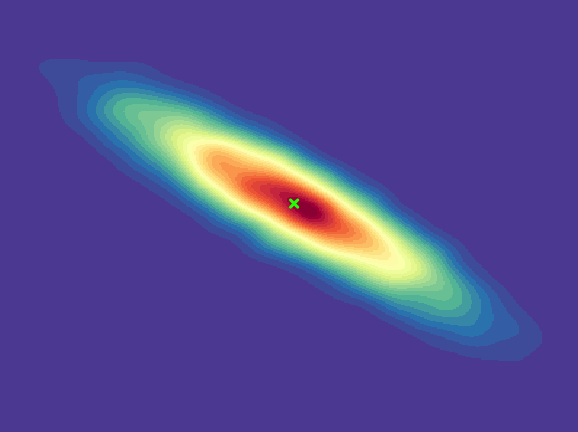
\includegraphics[width=0.6\textwidth]{figures/heatmap-log-linearity-SliceSampling-new-3}
	\caption{Approximated posterior density of the two dimensional log linearity constant of a two dimensional DPP with a uniform distribution as a prior. The MLE estimator is marked green and is at the mode of the distribution.}
	\label{fig:4.1}
\end{figure}

A further advantage over the MLE is that it might be possible to computationally approximate the posterior density, but not the MLE. This is typically the case if the log likelihood function is not concave, like in the setting of the MLE of the whole elementary kernel \(L\). In fact the only hard step in the calculation of the posterior \eqref{post} is the computation of the normalisation constant
\[\int\limits_{\Theta} f_{X,\Theta}(x, \theta) \nu(\mathrm{d}\theta). \]
This can often not be performed efficiently but the Markov chain Monte Carlo methods introduced later will yield an approximation of the posterior without the need to compute the normalisation constant.
\end{emp}

\begin{emp}[Regularisation through the prior]
The prior density is very closely related to the regulariser introduced in the section about maximum likelihood estimation. In fact the mode of the posterior \(f_{\Theta|X}\) is nothing else but the maximiser of 
\[\log(f_{\Theta|X}) = \mathcal L + R\]
where \(R = \log(f_\Theta)\) and hence nothing else but a regularised MLE. In fact if \(R\) is a regularisation and \(\exp(R)\) is integrable with respect to \(\mu\), then one can choose \(f_\Theta\propto \exp(R)\) as a prior density. Hence the proposition of a prior and a regulariser are equivalent in a wide variety of cases, but again, the posterior density encodes much more information than just the location of its mode which is the regularised MLE.
\end{emp}

\begin{emp}[Bayesian approach without prior]
We have seen that the prior is nothing else but a regularisation of the likelihood and since MLE can be carried out without regularisation it is natural to ask whether the Bayesian approach works without a prior. We have seen that if there is a uniform distribution on the parameter space, the unregularised MLE corresponds to the uniform distribution as a prior. So the question is what changes if we propose \(f_\Theta = 1\) as a prior if there is no uniform distribution, or more generally what happens if the prior \(f_\Theta\) has infinite integral.

In this case, the unnormalised posterior distribution 
\begin{equation}\label{genpost}
\mathfrak{f}(\theta) = f_{X|\Theta}(x| \theta) f_\Theta(\theta)
\end{equation}
might not have finite integral and can therefore not be normalised. Hence the posterior can not be seen as a probability density, but the generalised form \eqref{genpost} still exists. If we use the constant prior \(f_\Theta=1\), the generalised posterior \(\mathfrak{f}(\theta)\) is just the observation probability (or density if \(\mathcal X\) is continuous) of the data \(x\) under the parameter \(\theta\).
\end{emp}

\subsubsection*{Expression of the posterior for DPPs}

Now we will express the posterior in the case of DPPs under the following conditions.

\begin{emp}[Setting]
Let \((\Theta, \nu)\) be a measure space and \(L(\theta)\in\mathbb R^{N\times N}_{\text{sym}, +}\) be an elementary kernel for every \(\theta\in\Theta\). Further we assume that we have independent realisations \(Y_1, \dots, Y_n\) of a  \(L\)-ensemble.
\end{emp}

Typically the parametrisations \(\theta\mapsto L(\theta)\) will be one of the three parametric models in III.2.1, i.e. \(\theta\) will either be the whole kernel itself, the quality vector or the log linearity constant of the qualities and \(L(\theta)\) the associated elementary kernel.

The independence relation leads to a factorisation of the density and we obtain the following expression for the posterior density
\begin{equation}\label{post2}
f_{\Theta|\mathbf Y^n}(\theta|Y_1, \dots, Y_n) \propto f_\Theta(\theta) \prod_{i=1}^n f_{\mathbf Y|\Theta}(Y_i|\theta) = f_\Theta(\theta) \prod_{i=1}^n \frac{\det(L(\theta)_{Y_i})}{\det(L(\theta) + I)}.
\end{equation}

Unfortunately the normalisation constant
\begin{equation}\label{norma}
\int\limits_{\Theta} f_{\Theta|\mathbf Y^n}(\theta|Y_1, \dots, Y_n)\nu(\mathrm{d}\theta) = \int\limits_{\Theta} f_\Theta(\theta) \prod_{i=1}^n \frac{\det(L(\theta)_{Y_i})}{\det(L(\theta) + I)}\nu(\mathrm{d}\theta)
\end{equation}
can neither be computed analytically nor numerically in an efficient way since the evaluation of this density involves the computation of the determinant of a \(N\times N\) matrix. This problem can be solved through the powerful methods of Markov chain Monte Carlo simulation that allow to approximate a distribution with only the knowledge of its unnormalised density. 

\subsubsection{Model selection using the Bayes factor}

In this paragraph we will quickly touch on how the Bayesian approach can be used to compare two different models, i.e. two different parametric families \(\mathcal F_1\) and \(\mathcal F_2\) including two different priors \(f_{\Theta_1}\) and \(f_{\Theta_2}\). For this we will work in the following setup.

\begin{emp}[Setting]
Let \(\Theta_1, \Theta_2\) be measurable spaces and \(\nu_i\)  measures on \(\Theta_i\) for \(i=1, 2\). Let \(f_{\Theta_i}\colon \Theta_i\to[0, \infty]\) be probability densities with respect to \(\nu_i\), i.e.
\[\int\limits_{\Theta_i} f_{\Theta_i}(\theta)\nu_i(\mathrm{d}\theta) = 1 \quad \text{for } i = 1, 2.\]
Further let
\[\mathcal F_i = \Big\{ f_{X| \Theta_i}(\cdot |\theta) \;\big\lvert\; \theta\in\Theta_i\Big\}\]
by a family of probability densities with respect to \(\mu^n\coloneqq\prod_{i=1}^n\mu(\mathrm d x_i)\).
\end{emp}

The goal is now two compare which model \(\mathcal F_i\) in combination with the corresponding prior describes the phenomenon better given some data \(x\). For this we follow \cite{kass1995bayes} and introduce the \emph{Bayes factor} of the two models given the data \(x\) through
\[K \coloneqq K(\mathcal F_1, \mathcal F_2| x) \coloneqq\frac{f(x|\mathcal F_1)}{f(x|\mathcal F_2)} = \frac{\int_{\Theta_1} f_{X| \Theta_1}(x| \theta) f_{\Theta_1}(\theta)\nu_1(\mathrm{d}\theta)}{\int_{\Theta_2} f_{X| \Theta_2}(x| \theta) f_{\Theta_2}(\theta)\nu_2(\mathrm{d}\theta)}. \]
This is nothing but the ratio of the total probabilities of the data \(x\) under the respective models. If this ratio is big, the model \(\mathcal F_1\) including its prior can be seen as a better description of the data compared to the second model. There is no clear definition on when the ratio can be seen as big enough to say this, but the following guidelines in Table \ref{tab:BayesFactor} were proposed in \cite{kass1995bayes}.

\begin{table}
\centering
\begin{tabular}{ |c|c| } 
 \hline
  Value for \(K\) & Interpretation \\ \hline
 \(1 - 3.2\) & Only worth a bare mention \\ \hline
 \(3.2 - 10\) & Substantial \\ \hline
 \(10 - 100\) & Strong \\ \hline
 \(>100\) & Decisive \\ \hline
\end{tabular}
\caption{Interpretation of how strongly different Bayes factors imply that one model a better description of the data than the other one.} \label{tab:BayesFactor}
\end{table}

\section{Markov chain Monte Carlo methods}

The method of Markov chain Monte Carlo (MCMC) simulation arose almost as early as the Monte Carlo\footnote{A legend has it that the name Monte Carlo was given to the work of von Neumann and Ulam by a colleague referring to Ulam�s uncle who lost a significant amount of money gambling in the Monte Carlo casino in Monaco.} simulations itself and since then a rich theory has been established and a broad range of applications have been found. However, we can only give a short overview over the basic principles and refer to \cite{meyn2012markov} for an introduction of Markov chain theory and to \cite{robert2013monte} for a survey on (Markov chain) Monte Carlo methods. 

Our motivation for the study of MCMC methods was to obtain an approximation of a distribution \(\pi\) under the knowledge of its unnormalised density. In the nutshell the idea is to construct an ergodic Markov chain \((X_n)_{n\in\mathbb N}\) with stationary distribution \(\pi\), i.e. such that one has
\[ \hat{\mathbb P}_n =\frac1n \sum_{i=1}^n \delta_{X_n} \xlongrightarrow{n\to\infty} \pi \]
almost surely in the weak sense. 
This Markov chain can then be simulated using Monte Carlo methods and the associated empirical measures \(\hat{\mathbb P}_n\) will be approximations of \(\pi\). However, to explain this in more detail we need to recapture some notions of Markov chains.

\subsection{Reminder on Markov chains}

We will provide an extremely short presentation of only those results that we will use to explain the core of MCMC methods. However, this will not contain any proofs and hence it can not replace the study of the already mentioned text books.

Let in the following \((\mathcal X, \mathcal B(\mathcal X))\) be a measurable space. This will typically be a topological space with its Borel algebra later.


\begin{defi}[Markov chain]
\begin{enumerate}
\item A \emph{transition kernel} is a function \[K\colon\mathcal X\times\mathcal B(\mathcal X)\to[0, 1]\] such that
\begin{enumerate}
\item \(K(x, \cdot)\) is a probability measure for every \(x\in\mathcal X\) and
\item \(K(\cdot, A)\) is measurable for every \(A\in\mathcal B(\mathcal X)\).
\end{enumerate}
\item A \emph{Markov chain} with values in \(\mathcal X\) and transition kernel \(K\) is a collection \((X_n)_{n\in\mathbb N}\) of \(\mathcal X\) valued random variables such that
\begin{equation}\label{MC}
\mathbb P\big(X_0\in A_0, \dots, X_n\in A_n\big) = \int\limits_{A_0} \gamma(\mathrm{d}x_0) \int\limits_{A_1} K(x_0, \mathrm{d}x_1) \cdots \int\limits_{A_n} K(x_{n-1}, \mathrm{d}x_n)
\end{equation}
for all \(A_1, \dots, A_n\in\mathcal B(\mathcal X)\) where \(\gamma\) denotes the distribution of \(X_0\).
\end{enumerate}
\end{defi}

We will call \(\gamma\) the \emph{initial} or \emph{starting distribution} of the Markov chain and will denote the distribution of this Markov chain by \(\mathbb P_\gamma\) and the expectation with respect to it by \(\mathbb E_\gamma[\cdot]\). Further an easy application of Kolmogorov�s consistency theorem implies that there is a measure \(\mathbb P_\gamma\) on the \emph{path space} \(\mathcal X^{\mathbb N}\) that satisfies \eqref{MC} which shows the existence of a Markov chain given a transition kernel \(K\) and initial distribution \(\gamma\) (cf. \cite{le2016brownian}). If the initial distribution is deterministic, i.e. \(\gamma = \delta_x\) for one \(x\in\mathcal X\), then we also write \(\mathbb P_x\) for the distribution of the Markov chain.
We close this paragraph by introducing the notation
\[K^n(x, A) \coloneqq \mathbb P_x(X_n\in A) \]
which is consistent with \eqref{MC} for \(n=1\).

\subsubsection*{Irreducibility, recurrence and existence of stationary distributions}

From now on we will fix a reference measure \(\mu\) on \(\mathcal X\).

\begin{defi}[Irreducibility and recurrence]
\begin{enumerate}
\item We say a Markov chain is \emph{\(\mu\) irreducible} if for every \(A\in\mathcal B(\mathcal X)\) with \(\mu(A)>0\) there is an index \(n\in\mathbb N\) such that
\[\mathbb P_x(X_n\in A) = K^n(x, A) > 0 \quad \text{for all } x\in\mathcal X. \]
\item A Markov chain \((X_n)_{n \in\mathbb N}\) is called \emph{recurrent} if
\begin{enumerate}
\item there is a measure \(\mu\) on \(\mathcal B(\mathcal X)\) such that \((X_n)\) is \(\mu\)-irreducible and
\item for every \(A\in\mathcal B(\mathcal X)\) with \(\mu(A)>0\) the expected number of visits of \(A\) is infinite, i.e.
\[\mathbb E_x\left[\left\lvert \left\{ n\in\mathbb N \mid X_n\in A\right\} \right\rvert\right] = \infty \quad \text{for every } x\in A.\]
\end{enumerate}
\item A Markov chain is called \emph{Harris recurrent} if it is recurrent and the number of visits is almost surely infinite, i.e. for any \(A\in\mathcal B(\mathcal X)\) with \(\mu(A)>0\) we have
\[\mathbb P_x\left(\left\lvert \left\{ n\in\mathbb N \mid X_n\in A\right\} \right\rvert = \infty\right) = 1 \quad \text{for every } x\in A.\]
\end{enumerate}
\end{defi}

\begin{defi}[Stationary distribution]
Let \(\pi\) be a measure on \(\mathcal B(\mathcal X)\). We call \(\pi\) an \emph{invariant} or \emph{stationary distribution} of a Markov chain with kernel \(K\), if \(X_{n+1}\) is distributed according to \(\pi\) whenever \(X_n\) is distributed according to \(\pi\). This is equivalent to
\[\pi(A) = \int\limits_{\mathcal X} K(x, A)\pi(\mathrm d x) \quad \text{for all } A\in\mathcal B(\mathcal X). \]
\end{defi}

\begin{theo}[Existence of stationary distributions]
If \((X_n)_{n\in\mathbb N}\) is a recurrent Markov chain, there exists an invariant \(\sigma\)-finite measure which is unique up to a multiplicative factor.
\end{theo}

\subsubsection*{Convergence to the stationary distribution and ergodicity}

We will not introduce the notion of periodic and aperiodic Markov chains here, because it would distract us from our actual goal. However, we still present the following result that only holds for aperiodic Markov chains and refer to \cite{meyn2012markov} for further information. The reason why we present the theorem is that it explains how one can approximately sample from the stationary distribution of a Markov chain, namely it says that the distribution of \(X_n\) converges to the invariant distribution.

\begin{theo}[Convergence to stationary distribution]
Let \((X_n)_{n\in\mathbb N}\) be a Harris recurrent and aperiodic Markov chain with stationary distribution \(\pi\). Let further \(\gamma_n\) be the distribution of \(X_n\), then we have
\[\left\lVert \gamma_n - \pi \right\rVert_{TV} \xlongrightarrow{n\to\infty} 0 \]
non increasing. Here \(\left\lVert \cdot \right\rVert_{TV}\) denotes the total variation of a measure
\[\left\lVert \mu \right\rVert_{TV}\coloneqq \sup_{\mathcal E}\sum\limits_{E\in\mathcal E} \left\lvert \mu(E) \right\rvert\]
where the supremum is taken over all finite families of disjoint measurable sets.
\end{theo}

\begin{theo}[Ergodic theorem]\label{ergTheo}
Let \((X_n)_{n\in\mathbb N}\) be a Harris recurrent Markov chain with stationary probability distribution \(\pi\), then \((X_n)_{n\in\mathbb N}\) is \emph{ergodic}. This means that if 
\[\hat{\mathbb P}_n \coloneqq \frac1n \sum_{i=1}^n \delta_{X_i} \]
is the empirical measure, we almost surely have
\begin{equation}\label{ergo}
\int\limits_{\mathcal X} f(x) \hat{\mathbb P}_n(\mathrm dx) \xlongrightarrow{n\to\infty} \int\limits_{\mathcal X} f(x)\pi(\mathrm dx)
\end{equation}
for every \(\pi\) integrable function \(f\).
\end{theo}

In the particular case that \(\mathcal X\) is a topological space and \(\mathcal B(\mathcal X)\) is the Borel algebra and if \(\pi\) is a probability measure, we obtain the almost sure weak convergence of \(\hat{\mathbb P}_n\) towards \(\pi\). This means that the convergence in \eqref{ergo} almost surely holds for all continuous and bounded functions \(f\). Hence, \(\hat{\mathbb P}_n\) are approximations of the invariant distribution in the sense of weak convergence, which is metrisable for example by the L�vy-Prokhorov or the bounded dual Lipschitz metric (cf. \cite{dudley2010distances}).


\subsubsection*{Idea of Markov chain Monte Carlo methods}

The motivation of the study of Markov chain Monte Carlo methods was to approximate the posterior distribution \eqref{post2}. The idea is now to construct and then simulate a Markov chain \((X_n)_{n\in\mathbb N}\) such that the empirical measures \(\hat{\mathbb P}_n\) converge to the posterior.
\begin{defi}[MCMC methods]
A \emph{Markov chain Monte Carlo} (\emph{MCMC}) method for the simulation of a distribution \(\pi\) is any method that produces an ergodic Markov chain \((X_n)_{n\in\mathbb N}\) with stationary distribution \(\pi\).
\end{defi}

In order to achieve this we only have to construct a suitable Markov chain and check the requirements of the ergodic theorem. This means we want to construct a Harris recurrent Markov chain with invariant distribution \(\pi\) and we want to do this without having to compute the normalisation constant \eqref{norma}. We will now present two of the most common methods to do this which are the Metropolis-Hastings random walk and the method of slice sampling.

\subsection{Metropolis-Hastings random walk}

The Metropolis-Hastings random walk is arguably the most commonly used MCMC method and certainly one of the oldest. It was actually proposed in the early 1950s from researchers of the American nuclear programme in Los Alamos (cf. \cite{metropolis1953equation}). First we will touch on the theoretical aspects of this method and follow the presentation in \cite{robert2013monte}.

\enlargethispage{.2cm}
\begin{emp}[Setting]
Let \(\Theta\) be a measurable space, \(\mu\) a measure on that space and \(f\colon\mathcal X\to[0, \infty]\) a function with finite positive integral
\[Z \coloneqq \int\limits_{\mathcal X} f(x) \mu(\mathrm{d}x)\in(0, \infty).\]
Our goal is to find a Harris recurrent Markov chain with invariant distribution
\[\pi(A)\coloneqq \frac1Z \int\limits_A f(x)\mu(\mathrm dx). \]
Let further
\[\Big\{ f(\cdot|x) \;\big\lvert\; x \in\mathcal X\Big\}\]
be a family of probability distributions, which we call the \emph{proposal distributions}.
\end{emp}

\begin{emp}[The MH random walk]
Given the first states \(X_0 = x_0, \dots, X_n = x_n\) of the Markov, we define \(X_{n+1}\) as follows. Let \(Y\) be distributed according to \(f(\cdot|x_n)\mathrm d\mu\) and take one realisation \(y\) of \(Y\). Then set
\[X_{n+1}\coloneqq\begin{cases}\; y \quad & \text{with probability } \rho(x_n, y) \\\; x_n & \text{with probability } 1 - \rho(x_n, y) \end{cases} \]
where
\begin{equation}\label{threshold}
\rho(x, y) \coloneqq \min\left\{ \frac{f(y) f(x|y)}{f(x)f(y|x)}, 1\right\}.
\end{equation}
and \(\frac{a}{0} \coloneqq \infty\). The first step of the random walk, namely the sampling of \(y\) is called the \emph{proposal step} and the second one the \emph{accept-reject step}. In conclusion a single step of the MH random walk can be expressed in the following way. 
\begin{algorithm}
\caption{A single step of the MH random walk \label{alg:MH}}
\begin{algorithmic}[1]
\Require{Current state \(x_n\) of the MH random walk}
\State \(y\sim f(\cdot|x_n)\mathrm d\mu\)
\State \(a\sim \mathcal U([0, 1])\)
\If{\(a\le \rho(x_n, y)\)}
  \State \(x_{n+1}\gets y\)
\Else 
  \State \(x_{n+1}\gets x_n\)
\EndIf
\State\Return{\(x_{n+1}\)}
\end{algorithmic}
\end{algorithm}
\end{emp}

To see that the definition above indeed yields a Markov chain we convince ourselves that the transition kernel is given by
\[K(x, A) = \int\limits_A\rho(x, y)f(y|x) \mu(\mathrm dy) + (1 - m(x)) \delta_x(A)\]
where \(\delta_x\) is the Dirac measure in \(x\) and
\[m(x) = \int\limits_{\mathcal X} \rho(x, y) f(y|x) \mu(\mathrm dy)\in[0, 1] \]
is the \emph{acceptance probability} of the chain at state \(x\).

\begin{prop}[Stationary distribution]
The probability measure \(\pi\) is a stationary distribution of the MH random walk.
\end{prop}
\begin{proof}
We have
\begin{equation}\label{calc1}
\begin{split}
\int\limits_{\mathcal X} K(x, A) \pi(\mathrm dx) & =  \frac1Z \int\limits_{\mathcal X}\left( \int\limits_A \rho(x, y) f(y|x) \mu(\mathrm dy) + (1 - m(x)) \delta_x(A)\right) f(x) \mu(\mathrm dx) 
\end{split}
\end{equation}
We note that
\[\rho(x, y) f(y|x) f(x) = \rho(y, x) f(x|y) f(y).\]
Furthermore we can compute
\begin{equation*}
\begin{split}
 \int\limits_{\mathcal X} m(x) \delta_x(A) f(x) \mu(\mathrm dx) & = \int\limits_{A}\int\limits_{\mathcal X} \rho(x, y) f(y|x) \mu(\mathrm dy) f(x) \mu(\mathrm dx) \\
 & =\;\int\limits_{\mathcal X} \int\limits_A \rho(x, y) f(y|x)f(x) \mu(\mathrm dx) \mu(\mathrm dy) \\
 & =\;\int\limits_{\mathcal X} \int\limits_A \rho(y, x) f(x|y) \mu(\mathrm dx) f(y) \mu(\mathrm dy)
\end{split}
\end{equation*}
where we used Fubini-Tonelli theorem\footnote{The Fubini-Tonelli theorem states that the order of integration with respect to two \(\sigma\)-additive measures can be swapped, if the integrated function is non negative.} in the second to last step. We note that two of the terms in \eqref{calc1} cancel out and we obtain
\[\int\limits_{\mathcal X} K(x, A) \pi(\mathrm dx) = \frac1Z \int\limits_{\mathcal X} \delta_x(A) f(x) \mu(\mathrm dx) = \pi(A). \]
\end{proof}

Now we aim to prove that the MH random walk is Harris recurrent because then the ergodic theorem yields that the empirical measures associated with the Markov chain will actually converge to \(\pi\). Obviously this is not trues for all proposal families in general the case, for example we could consider the case where the proposal distribution \(f(\cdot|x)\) is just the Dirac measure in \(x\).\footnote{Obviously this is slightly formal, because the Dirac measure can typically not be expressed through a density. However, rigorous examples can be constructed similarly.} Then the MH random walk would never leave its initial position which will typically be a deterministic point. Hence, the empirical measures are only the Dirac measure in the starting point and will not converge towards \(\pi\).

The first step towards Harris recurrence is to show irreducibility and this will already give us some hints to what families of proposal are sensible.

\begin{prop}[Irreducibility]
Assume that the proposal family is strictly positive, i.e.
\[f(y|x) > 0 \quad \text{for all } x, y\in\mathcal X. \]
Then the MH random walk is \(\pi\) irreducible.
\end{prop}
\begin{proof}
For any measurable set \(A\subseteq\mathcal X\) with positive measure \(\pi(A)>0\) we have
\[K(x, A) \ge \int\limits_A \rho(x, y)f(y|x) \mu(\mathrm d y) > 0. \]
To see this, we can assume that this would not hold and then the integrant has to be zero \(\mu\) almost surely. Since \(f(y|x)\) is strictly positive this would imply \(\rho(x, y) = 0\) and hence \(f(y) = 0\) for \(\mu\) almost all \(y\in A\). However, this is a contradiction to
\[\pi(A) = \int\limits_A f(y)\mu(\mathrm dy) > 0.\]
\end{proof}

Now we can formulate the ergodicity for \(\pi\) irreducible MH random walks.

\begin{theo}[Ergodicity of the MH random walk]
If the MH random walk is \(\pi\) irreducible, then it is also Harris recurrent and hence ergodic.
\end{theo}
\begin{proof}
We refer to Lemma 7.3 in \cite{robert2013monte} for the proof of Harris recurrency, the ergodicity then follows from the ergodic theorem.
\end{proof}

\subsubsection*{Implementation of the MH random walk}

So far we have presented the theoretical foundations of the MH random walk and now we want to touch on a few aspect of the simulation of this Markov chain. For this part we shall point the reader towards the example based introductions \cite{robert1999metropolis} and \cite{robert2010introducing} to the implementation of the MH random walk which also provide coding examples. We have seen that the empirical measures associated with the MH random walk converge to \(\pi\) under fairly mild assumptions, meaning for a wide class of proposal distributions. Nevertheless it is mostly the choice of the proposal that determines the speed of this convergence. 
 In order to shortly demonstrate this effect, we consider the case \(\mathcal X = \mathbb R^d\) and that the reference measure \(\mu\) is the Lebesgue measure.

\begin{emp}[Choosing a proposal family]
Usually one chooses the proposal such that the expectation of \(f(\cdot|x)\) is \(x\). The most common choice of a proposals is a family of normal distributions \(f(\cdot|x)\) with expectation \(x\) and covariance \(\Sigma\in\mathbb R^{d\times d}\). This also has the effect that the acceptance ratio takes the easier form
\[\rho(x, y) = \min\left\{ \frac{f(y)}{f(x)}, 1\right\}.\]
Also since the densities are strictly positive we ensure that the resulting Markov chain is \(\pi\) irreducible.
\end{emp}

\begin{emp}[Acceptance rate, autocorrelation and effective sample size]
Once we have agreed to stick to normal densities for the proposal distributions, we still have the freedom to choose the covariance \(\Sigma\in\mathbb R^{d\times d}\). This determines how far the proposed new values will be away from the current state of the Markov chain. The motivation for an aggressive proposal distribution, i.e. for a high variance would be that this would enable the Markov chain to take bigger steps and hence explore the space \(\mathcal X\) faster. Also the chain would be more likely to jump between possibly isolated areas of high density. However, this could also lead to a high rejection rate\footnote{The term should be rather intuitive; the rejection rate is the relative amount of rejections that occurred in the MH random walk and analogously the acceptance rate is its counterpart.} if the proposed values are often so far away from the current state of the Markov chain that they are lie within an area of low density. In this case the Markov chain will only �visit� few distinct points in the space \(\mathcal X\) which is also very unfavourable. In fact the findings in \cite{roberts1997weak} suggests that an acceptance rate around \(25\%\) is desirable in dimension \(d\ge3\) and around \(50\%\) for dimension \(d=1, 2\). The connection between the proposal distribution and the acceptance rate is also elaborated in the upcoming example.

The \emph{autocorrelation function} (\(\operatorname{acf}\)) of a sequence of data points \(x_0, \dots, x_n\) captures the estimated correlation between the observations. More precisely \(\operatorname{acf}(k)\) gives the empirical correlation\footnote{This is the correlation of the two empirical measures associated with \((x_0, \dots, x_{n-k})\) and \((x_k, \dots, x_n)\).} of \((x_0, x_1, \dots, x_{n-k})\) and \((x_k, x_{k+1}, \dots, x_n)\). In the case that the data points are generated by a MH random walk, the autocorrelation function determines the correlation of the Markov chain at time \(l\) with the Markov chain at time \(l+k\). Hence, if \(\operatorname{acf}(k)<\varepsilon_0\) where \(\varepsilon_0>0\) is fixed in advance, one can perceive \(x_0, x_k, x_{2k}, \dots\) as an independent sequence of samples from \(\pi\)  -- or more precisely an only weakly correlated one. The \emph{effective sample size} is the length \(m\) of this new almost uncorrelated sequence \(x_0, x_k, x_{2k}, \dots, x_{mk}\). Obviously the effective sample size strongly depends on the choice of \(\varepsilon_0\) that incorporates how much correlation one is willing to accept.

We should quickly touch on how the proposal affects the autocorrelation function and hence the effective sample size. Assume we have a very aggressive proposal distribution. Then we will typically have a high rejection rate and hence \(x_l = x_{l+k}\) a lot of times meaning that the autocorrelation function will be high and therefore the effective sample size is rather low. On the other hand if the proposal is too conservative the MH random walk will only take very small steps and hence \(x_{l+k}\) will still be close to \(x_l\). Therefore, the autocorrelation will be high and the effective sample size low again. This effect of the proposal can be seen in Figure \ref{fig:4.1.2}.
\end{emp}

\begin{ex}[One dimensional MH]\label{example}
We follow an examples for a one dimensional MH random walk given in \cite{robert1999metropolis} and we want to approximate the probability distribution with unnormalised density
\[f(x)\coloneqq \sin(x)^2\cdot\sin(2x)^2\cdot\exp\left(-\frac{x^2}{2}\right). \]
The goal of this example is to see how different proposal distributions lead to different acceptance rates, a different exploration of the state space \(\mathcal X = \mathbb R\) and different effective sample sizes. In order to achieve this, we run \(2\cdot10^4\) samples of the MH random walk with starting point \(x_0=1\) and three different values \(\alpha = 0.01, 3, 100\) for the variance of the proposal distributions. Then we plot a histogram including the actual density and the autocorrelation function for all different values. The acceptance rates where approximately \(88\%\) for \(\alpha=0.01\), \(34\%\) for \(\alpha=3\) and \(9\%\) for \(\alpha=100\). The effective sample sizes for the three different chains different values for \(\alpha\) 
are
\[\frac{2\cdot10^4}{50} = 4\cdot10^2, \quad \frac{2\cdot10^4}{8} = 2.5\cdot10^3 \quad \text{and } \frac{2\cdot10^4}{30} \approx 7\cdot10^2 \]
for \(\alpha=0.01, 3, 100\) respectively.

This simulation illustrates the problem of too aggressive -- \(\alpha = 100\) -- and too conservative -- \(\alpha=0.01\) -- proposal distributions and shows how this effects the acceptance rate and the effective sample size.

\begin{figure}[h!]
	\centering
	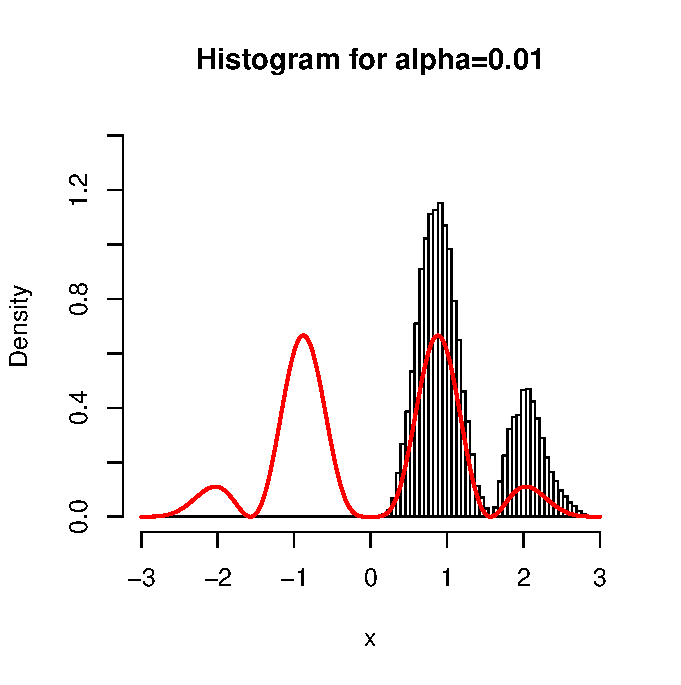
\includegraphics[width=0.41\textwidth]{figures/alpha-small}
	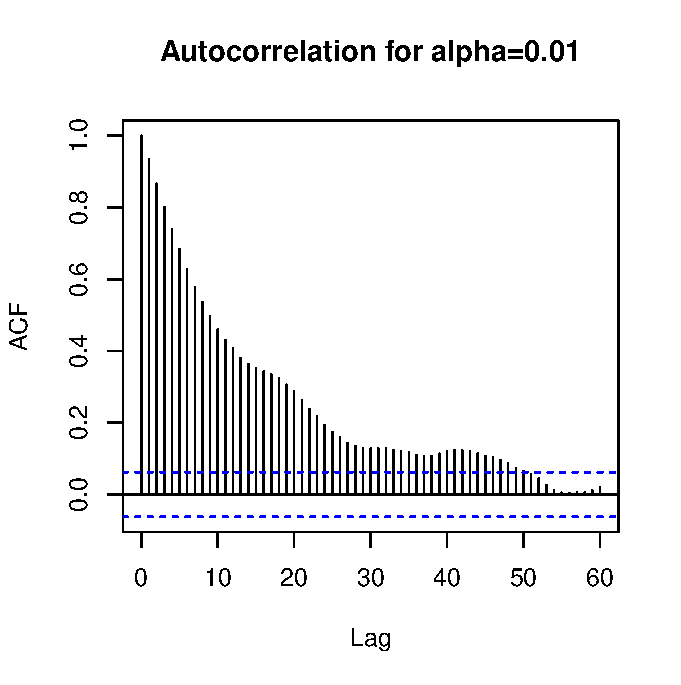
\includegraphics[width=0.41\textwidth]{figures/auto-alpha-small}
	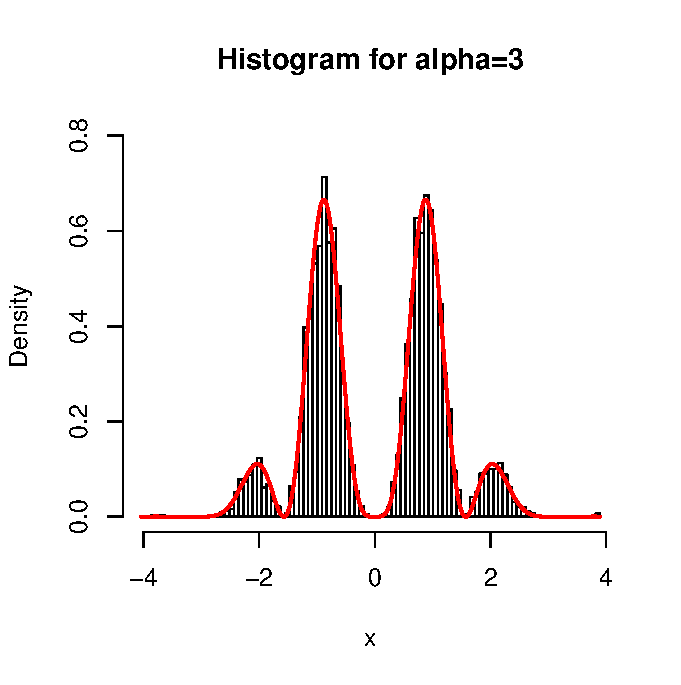
\includegraphics[width=0.41\textwidth]{figures/alpha-optimal}
	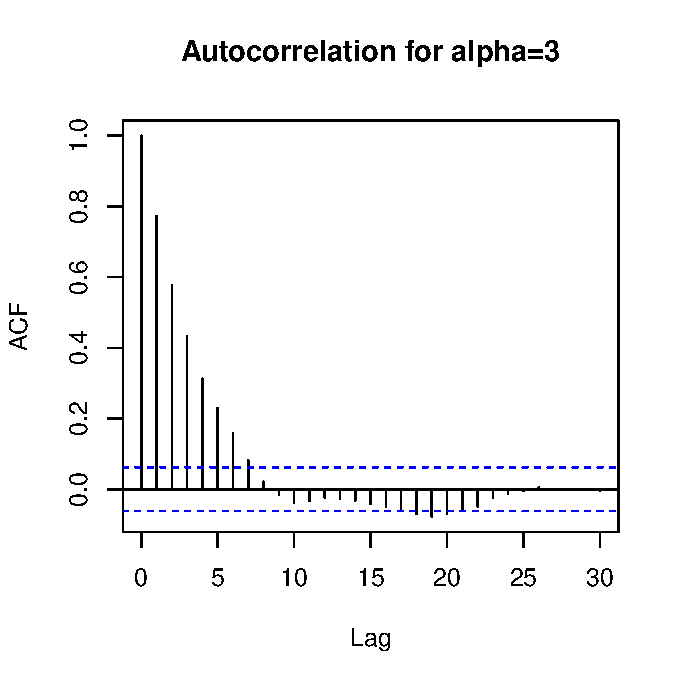
\includegraphics[width=0.41\textwidth]{figures/auto-alpha-optimal}
	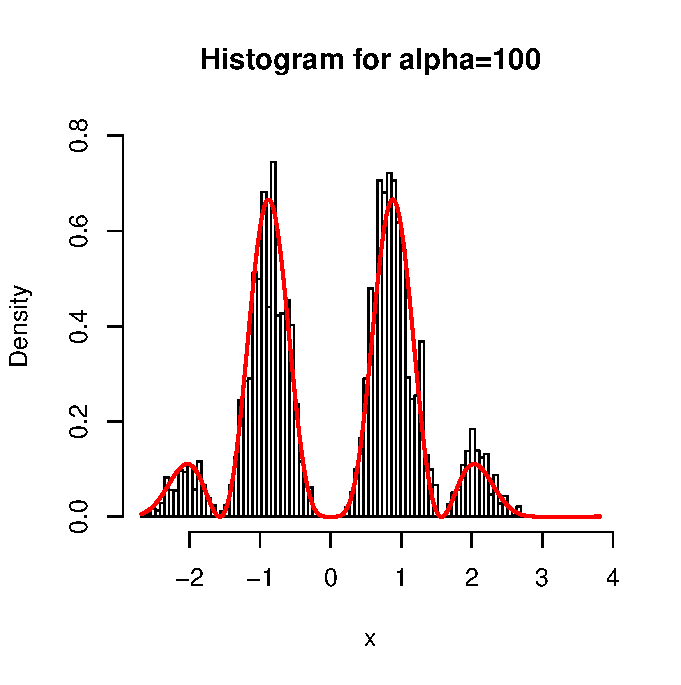
\includegraphics[width=0.41\textwidth]{figures/alpha-big}
	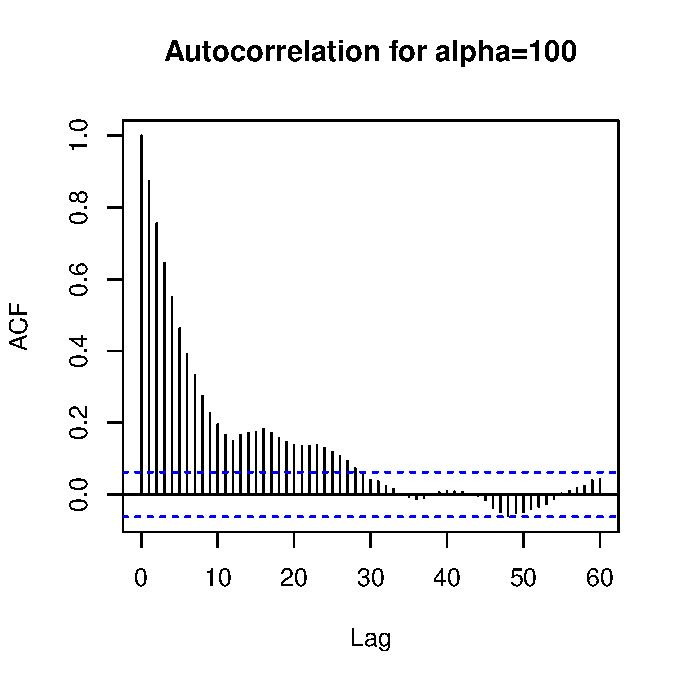
\includegraphics[width=0.41\textwidth]{figures/auto-alpha-big}
	\caption{Histograms and autocorrelation functions of for three different variances \(\alpha\) of the Gaussian proposal distributions. It is apparent that the histogram for \(\alpha=3\) fits the actual density the best and also that the autocorrelation decays the quickest for this parameter. Note that for \(\alpha=0.01\) the MH random walk only explored some area of high density. The actual density is obtained by numerical integration.}
	\label{fig:4.1.2}
\end{figure}

\end{ex}

\begin{emp}[Tuning the proposal]\label{tuning}
In order to obtain a higher acceptance rate without simply choosing the variance of the proposal distribution small one can \emph{tune} or \emph{adapt} the proposal distribution. This means one adjusts the proposal distribution after a while, lets say after the first \(10^3\) samples in such a way that one replaces the original covariance matrix \(\Sigma\) by the empirical covariance of the first \(10^3\) samples. Then one forgets about all the samples so far -- they are usually called the \emph{burn in period} -- and starts a new MH random walk. It is essential to drop the first samples since otherwise the Markov property would break as all further samples now rely on the coveriance of the first burn in period and hence on those points. 
The reason why this increases the acceptance rate is, that the proposal now only is aggressive in those directions where the mass of the density is widely spread. For a further discussion we refer to \cite{roberts2009examples}.
\end{emp}

\begin{emp}[The Gelman-Rubin diagnostic]
So far we have seen guidelines as what properties of the MCMC simulation can be seen as favourable or not. However those comments can not replace quantitative measures on the convergence of the simulated Markov chains and one of them is the Gelman-Rubin diagnostics which is also called the \(\hat R\) value. We will not be able to rigorously introduce this quantity, but will make a few comments since we will use it later and refer to \cite{robert2012discretization} for a thorough introduction to convergence diagnostics for MCMC methods and to \cite{gelman1992inference} and \cite{brooks1998general} for the orinigal work by Gelman, Rubin and Brooks. In a nutshell the \(\hat R\) value is an estimate of how much longer a MCMC simulation would have to run to be a good approximation of the stationary distribution. It is generally accepted that a \(\hat R\) value of at most \(1.05\) can be taken as a sign -- but not a proof -- of convergence, cf. \cite{brooks1998general}.

Although we don�t introduce the statistics itself, we shall present the requirements to compute it. The procedure one has to take is the following:
\begin{enumerate}
\item Find the possibly multiple modes of the distribution that should be approximated. This can be done either by exploiting optimisation algorithms or running short MCMC simulations, which we will do later in our toy example.
\item Run \(m\) MCMC simulations of length \(n\) starting at random points with variance greater than the estimated variance of the target distribution \(\pi\). This variance is typically estimated through a first, shorter MCMC simulation which can also be used to tune the proposal.
\end{enumerate}
Now the \(\hat R\) value can be computed from the entirety of those \(m\) chains of length \(n\) and we will rely on a pre-implemented tool in R to do this.
\end{emp}

\subsection{Slice sampling}

Slice sampling is a different MCMC method and quite similar to the MH random walk. Nevertheless it has the benefit that one does not have to define or tune a family of proposal distributions and that the constructed Markov chain is always irreducible. However, we will see that at least when one wants to simulate the slice sampling one runs into similar problems of having to choose a parameter that influences the auto correlation function and hence the speed of convergence of the method. We begin by fixing our frame we will work in.

\begin{emp}[Setting]
Let \(\mathcal X\) be a measurable space, \(\mu\) a measure on that space and \(f\colon\mathcal X\to[0, \infty]\) a function with finite integral
\[Z \coloneqq \int\limits_{\mathcal X} f(x) \mu(\mathrm{d}x)\in(0, \infty).\]
In particular there is \(\hat x\in\mathcal X\) such that \(f(\hat x)>0\). Our goal is to find an ergodic Markov chain with invariant distribution
\[\pi(A)\coloneqq \frac1Z \int\limits_A f(x)\mu(\mathrm dx). \]
Further we will assume -- after an eventual modification of \(f\) on a \(\mu\) Null set -- that 
\[f\le \left\lVert f \right\rVert_{L^\infty(\mu)} = \inf \Big\{ \alpha\in\mathbb R \;\big\lvert\; f \le \alpha \text{ almost surely with respect to } \mu \Big\}\in[0, \infty]. \]
\end{emp}

\begin{emp}[The slice sampling method]
Assume we have already given the first \(n\) samples \(x_1, \dots, x_n\) of the Markov chain. If we have \(f(x_n)=0\), then we set \(x_{n+1}\coloneqq \hat x\). Otherwise we sample \(y\) according to the uniform distribution on \([0, f(x_n)]\) and define the \emph{slice}
\[S\coloneqq S(y)\coloneqq \left\{ x\in\mathcal X \mid f(x) \ge y \right\}. \]
\begin{figure}[h!]
	\centering
	\includegraphics[width=0.6\textwidth]{figures/Slice-sampling-neal-new}
	\caption{Schematic sketch of the selection of a slice: (a) first \(y\) is sampled uniformly in \([0, f(x_0)]\) and (b) the slice is selected. Original graphic from \cite{neal2003slice}.}
	\label{fig:4.2}
\end{figure}

Note that because \(y < f(x_n)\le \left\lVert f \right\rVert_{L^\infty(\mu)}\) holds almost surely, we have \(\mu(S)>0\) as well as
\[ \mu(S) \le y^{-1} \int\limits_S f(x)\mu(\mathrm dx)<\infty \]
where we used Markov�s inequality as well as \(y>0\) almost surely. Now draw \(x_{n+1}\) according to the uniform distribution\footnote{Of course we mean the uniform distribution with respect to \(\mu\) that gives weight \(\mu(S)^{-1} \cdot \mu(A)\) to a set \(A\subseteq S\).} on \(S\). Note that if \(f(x_n)>0\), then \(f(x_{n+1})\ge y > 0\) almost surely, hence \(f(x_n) = 0\) can only hold for \(n=0\). Further the reason why we have to treat the case \(f(x_n)=0\) individually is, that there typically is no uniform distribution on the slice \(S(0) = \mathcal X\).
The pseudo code for the construction of the resulting Markov chain is presented in Algorithm \ref{alg:slice-sampling}.
\begin{algorithm}
\caption{A single slice sampling step \label{alg:slice-sampling}}
\begin{algorithmic}[1]
\Require{Current state \(x_n\) of the Markov chain}
 \If \(f(x_n) = 0\)
  \State \(x_{n+1}\gets \hat x\)
\Else
  \State \(y\sim \mathcal U([0, f(x_n)])\)
  \State \(S\gets \left\{ x\in\mathcal X \mid f(x) \ge y \right\}\)
  \State \(x_{n+1} \sim \mathcal U(S)\)
\EndIf
\State\Return{\(x_{n+1}\)}
\end{algorithmic}
\end{algorithm}
\end{emp}

If we compare the Markov chain to the MH random walk, we notice that in the slice sampling we first create a random threshold \(y\) and then sample uniformly from all points that satisfy this threshold. This is just the other way round than in the MH random walk where we first make a proposal for the next state of the Markov chain and then decide whether we will accept it or not.

Just like in the case of the MH random walk we can explicitly give the transition kernel and use this expression then to check that \(\pi\) is a stationary distribution. The kernel of the Markov chain that arises from the slice sampling iteration is given by
\begin{equation*}
\begin{split}
K(x, A) & = \int\limits_\mathbb R\frac{\mathds{1}_{[0, f(x)]}(y)}{f(x)} \cdot \frac{\mu(A\cap S(y))}{\mu(S(y))} \lambda(\mathrm dy) \\
& = \int\limits_\mathbb R\frac{\mathds{1}_{[0, f(x)]}(y)}{f(x)} \cdot \frac1{Z(y)}\int\limits_A \mathds{1}_{[y, \infty)}(f(z)) \mu(\mathrm dz) \lambda(\mathrm dy)
\end{split}
\end{equation*}
where \(\lambda\) is the Lebesgue measure on \(\mathbb R\), \(\mathds{1}\) is the indicator function and \(Z(y)\) is the normalisation constant
\[Z(y)\coloneqq \int\limits_{\mathcal X} \mathds{1}_{[y, \infty)}(f(z)) \mu(\mathrm dz) = \mu(S(y)) \in(0, \infty). \]
Obviously the expression above only holds if \(f(x)>0\) and in the case \(f(x) = 0\) we have
\[K(x, A) = \delta_{\hat x}(A).\]

\begin{prop}[Invariant distribution]
The probability distribution \(\pi\) is a stationary distribution of the Markov chain associated with the slice sampling method.
\end{prop}
\begin{proof}
For any \(A\subseteq\mathcal X\) we can compute
\begin{equation*}
\begin{split}
\int\limits_{\mathcal X} K(x, A) \pi(\mathrm dx) & = \frac1Z\int\limits_{\mathcal X }\int\limits_\mathbb R\frac{\mathds{1}_{[0, f(x)]}(y)}{f(x)}\cdot \frac1{Z(y)} \int\limits_A \mathds{1}_{[y, \infty)}(f(z)) \mu(\mathrm dz) \lambda(\mathrm dy) f(x) \mu(\mathrm dx) \\
& =\frac1Z \int\limits_{ A }\int\limits_\mathbb R \frac1{Z(y)} \int\limits_{\mathcal X}\mathds{1}_{[y, \infty)}(f(x)) \mu(\mathrm dx) \mathds{1}_{[0, f(z)]}(y) \lambda(\mathrm dy) \mu(\mathrm dz) \\
& = \frac1Z\int\limits_A f(z)\mu(\mathrm dz) = \pi(A)
\end{split}
\end{equation*}
where we again used Fubini�s theorem for non negative functions.
\end{proof}

\begin{prop}[Irreducibility]
The Markov chain that arises from the slice sampling algorithm is \(\pi\) irreducible.
\end{prop}
\begin{proof}
Fix \(A\subseteq\mathcal X\) with positive probability \(\pi(A)>0\) and \(x\in\mathcal X\). If we have \(f(x)>0\), then we have \(\mu(A\cap S(y))>0\) for one \(y\in(0, f(x))\). We obtain
\[K(x, A) \ge \int\limits_{\mathbb R} \frac{\mathds{1}_{[0, y]}(z)}{f(x)} \cdot \frac{\mu(A\cap S(z))}{\mu(S(z))}> 0. \]
If however \(f(x)=0\), then we get
\[K^2(x, A) = K(\hat x, A) > 0. \]
\end{proof}

\begin{theo}[Ergodicity]
If \(f\) is bounded, the Markov chain induced by the slice sampling method is ergodic.
\end{theo}
\begin{proof}
See Theorem 6 in \cite{mira2002efficiency}.
\end{proof}

\subsubsection*{Implementation details}

Just like in the case of the MH random walk we will make a few comments about the actual simulation of the slice sampling algorithm and for this, we will assume \(\mathcal X\subseteq\mathbb R^d\).

The main difficulty in the implementation is the sampling of a uniform distribution on a slice \(S\). In practice it is not even possible to calculate the slice but one can exploit the following observation. Assume that we are able to simulate a uniform distribution on a set \(C\) that contains the slice \(S\). Then the following algorithm -- which is nothing but the conditioning of this uniform distribution on the event that the outcome is in \(S\) -- samples uniformly from \(S\).
\begin{algorithm}
\caption{Sampling from a uniform distribution on a subset \(S\subseteq C\) \label{alg:slice-sample}}
\begin{algorithmic}[1]
\Require{\(S\) and \(C\supseteq S\)}
\State \(x\sim\mathcal U(C)\)
\While {\(x\notin S\)}
  \State \(x\sim\mathcal U(C)\)
\EndWhile
\State\Return{\(x\)}
\end{algorithmic}
\end{algorithm}

An obvious choice for \(C\) would be a cuboid 
\[C = \prod_{i = 1}^d [a_i, b_i]\]
since it is straight forward to sample from a uniform distribution on a cuboid. Namely one only has to sample the individual coordinates uniformly in the intervals \([a_i, b_i]\). The problem still remains how one can find a cuboid that surely contains the whole slice \(S\). The short answer is that there is no general way to do this. However, not everything is lost, since we can use random cuboids that have the property that every part of the slice is contained in the cuboid with positive probability. This will be crucial in retaining the irreducibility of the Markov chain. In fact it has been found that in applications the following procedure works well (cf. \cite{affandi2014learning}). Given the current state \(x_n\) of the Markov chain, we propose a random interval \([a_i, b_i]\) around the \(i\)-th component of \(x_n\). Then we extend those intervals until the endpoints \(a\) and \(b\) of the cuboid do not lie in the slice anymore which is described in Algorithm \ref{alg:cuboid}.
\begin{algorithm}
\caption{Sampling a random cuboid \label{alg:cuboid}}
\begin{algorithmic}[1]
\Require{Current state \(x_n\) of the Markov chain, parameter \(\alpha>0\)}
\For {\(i=1, \dots, d\)}
  \State \(a_i, b_i \sim \mathcal E(\alpha)\)
\EndFor
\State \(a\gets (a_1, \dots, a_d), b\gets(b_1, \dots, b_d)\)
\While {\(x - a \in S\)}
  \State \(a \gets 2 \cdot a\)
\EndWhile
\While {\(x + b \in S\)}
  \State \(b \gets 2 \cdot b\)
\EndWhile
\State\Return{\((x - a, x + b)\)}
\end{algorithmic}
\end{algorithm}

Here \(\mathcal E(\alpha)\) denotes the exponential distribution with parameter \(\alpha\) and determines how large the first proposed intervals are. It is straight forward and computationally very easy to determine whether a point \(x\) is in the slice \(S(y)\) since one only has to check \(f(x) \ge y\). The reason for the choice of the exponential distribution is that this ensures that the cuboid can get arbitrarily large with positive probability. This leads to the effect that the Markov chain one obtains in exchanging the sample from \(\mathcal U(S)\) by a sample from \(\mathcal U(S\cap C)\) still is irreducible. To see this we can slightly modify the proof of irreducibility, so for \(A\subseteq\mathcal X\) with positive probability we choose \(y>0\) such that \(\mu(A\cap S(y))>0\). Further we can choose a cuboid \(C\) around \(x\) such that \(\mu\big(A\cap S(y)\cap C\big)>0\). Further this cuboid is contained in the cuboid proposed by Algorithm \ref{alg:cuboid} with positive probability and hence we have
\[K(x, A) = \mathbb P_x(X_1\in A) > 0. \]
The algorithm that arises from the combination of the usual slice sampling method and the approximation of the uniform distribution on the slice is presented in Algorithm \ref{alg:slice-sampling-implementation}.
\begin{algorithm}
\caption{Algorithm for the slice sampling \label{alg:slice-sampling-implementation}}
\begin{algorithmic}[1]
\Require{Unnormalised density \(f\), starting value \(x_0\), desired length \(n\) of the chain, \(\alpha>0\)}
\If {\(f(x_0) = 0\)}
  \State \(x_0 \gets \hat x\)
\EndIf
\For {\(i = 0, \dots, n-1\)}
  \State \(y\sim \mathcal U([0, f(x_{i})])\)
  \State \(C\) random cuboid around \(x_{i}\) with parameter \(\alpha\)
  \State \(x\sim\mathcal U(C)\)
  \While {\(f(x)<y\)}
    \State \(x\sim\mathcal U(C)\)
  \EndWhile
  \State \(x_{i+1} \gets x\)
\EndFor
\State\Return{\(x = (x_0, \dots, x_n)\)}
\end{algorithmic}
\end{algorithm}
It shall be noted, that this algorithm also uses a point \(\hat x\) of positive density, which can be determined easily for a lot of densities \(f\). If this is not straight forward, one can sample \(x_0\) according to a normal distribution until we select a point of positive density.

Obviously the algorithm presented above produces a Markov chain that is not identical with the one presented in the theoretical discussion of the slice sampling method. However, if one wants to ensure the convergence of this slightly modified Markov chain, one has to check whether \(\pi\) remains a stationary distribution and whether the chain is still ergodic. This is usually done in the specific setting one works in, cf. \cite{neal2003slice}. We will quickly discuss this in a very easy case. Namely let us assume \(d=1\) and that \(f\) is continuous and has only one local maximum. We call \(f\) \emph{unimodal} in this case and note that every slice \(S(y)\) is an interval. Hence, the proposed cuboid is an interval around \(x_n\in S(y)\) such that both endpoints are outside of the slice \(S(y)\) and hence we have \(S(y)\subseteq C\). Therefore, the algorithm above is equivalent to the original slice sampling method and hence produces an ergodic Markov chain with the desired invariant distribution.

\begin{emp}[The choice of \(\alpha\)]
One could think that a small choice of \(\alpha\) -- which relates into large values of \(a_i\) and \(b_i\) -- would be the best since this increases the probability that the whole slice \(S\) is contained in the cuboid \(C\). There is some truth in this approach, since \(\mathcal U(S\cap C)\) is a better approximation of \(\mathcal U(S)\) if \(C\) is larger and further the while loops in Algorithm \ref{alg:cuboid} need less repetitions if \(a_i\) and \(b_i\) initially are big. However, one should not choose \(\alpha\) too small, because a large cuboid \(C\) also means that a lot of samples from \(\mathcal U(C)\) will lie outside of \(S\cap C\). Hence, Algorithm \ref{alg:slice-sample} that samples from \(\mathcal U(S\cap C)\) will get slower as it will reject a lot of samples.

In conclusion there is a trade off in terms of computation time between the choice of too small and too large values for \(\alpha\). However not always the parameter \(\alpha\) that minimises the simulation time is the most suitable, since the autocorrelation decreases together with the parameter \(\alpha\). Hence, computation time should rather be compared to the effective sample size.

Those effects of \(\alpha\) on the auto correlation and therefore effective sample size can be seen in Figure \ref{fig:4.3} where the procedure of Example \ref{example} is repeated but this time with the slice sampling method. The sample size remains \(2\cdot10^4\) and the different parameter choices where \(\alpha = 0.01, 0.5, 10\). The according computation times where approximately \(26\si{s}\) for \(\alpha=0.01\), \(1.7\si{s}\) for \(\alpha=0.5\) and \(1.7\si{s}\) for \(\alpha=10\). In regard of the decay of the autocorrelation functions and the resulting effective sample sizes, it is apparent that the choice \(\alpha = 0.5\) would be the most sensible one in this case.

\begin{figure}[h!]
	\centering
	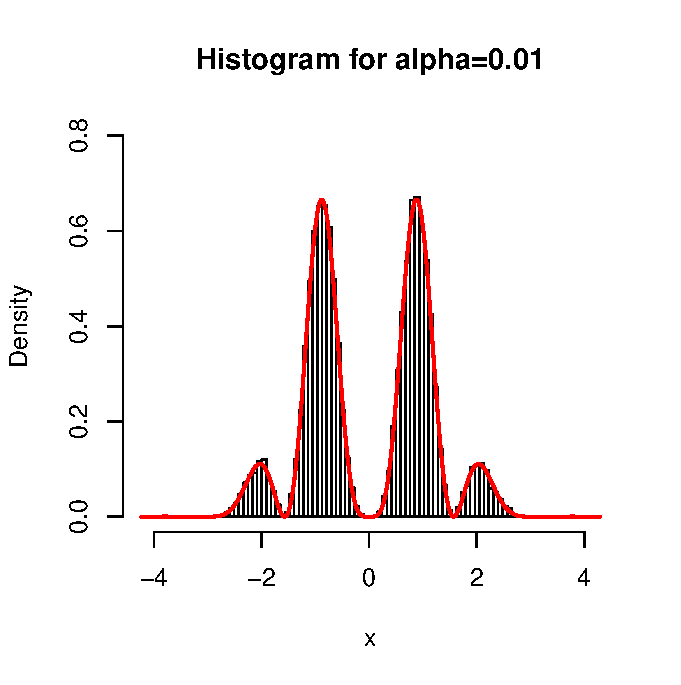
\includegraphics[width=0.44\textwidth]{figures/slice-alpha-small}
	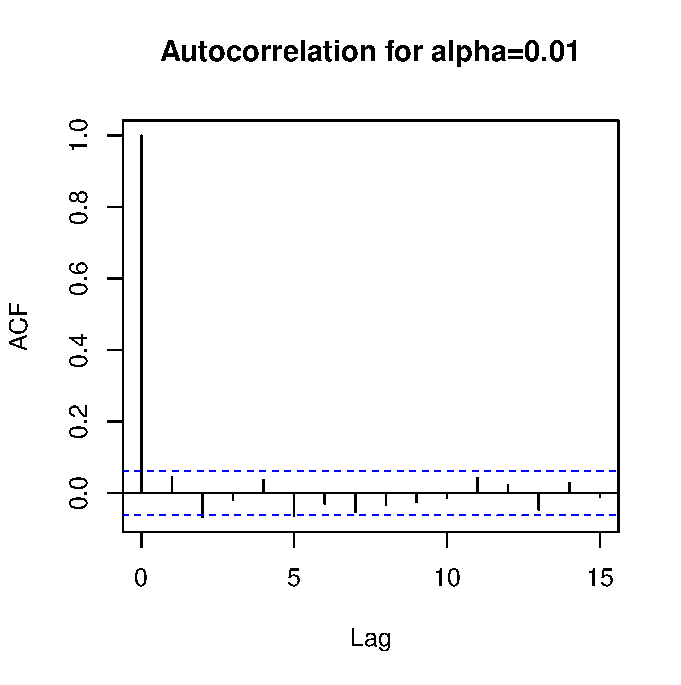
\includegraphics[width=0.44\textwidth]{figures/slice-auto-alpha-small}
	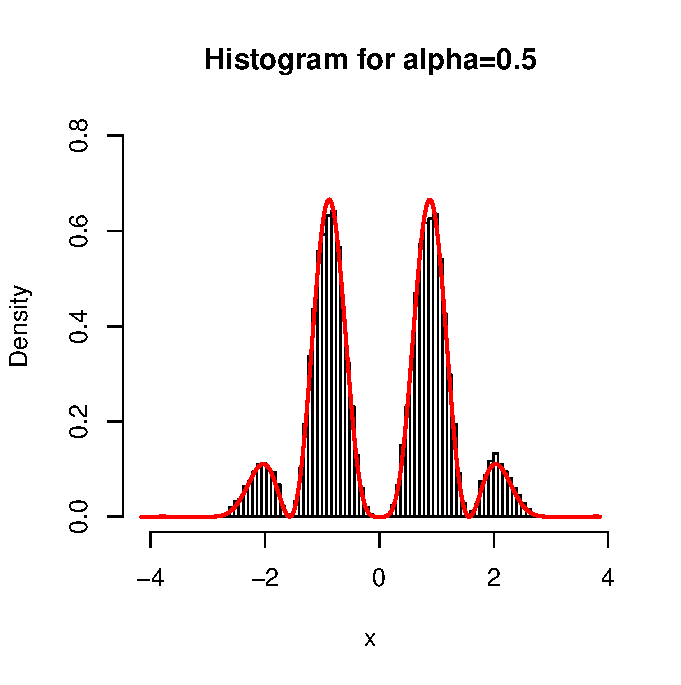
\includegraphics[width=0.44\textwidth]{figures/slice-alpha-optimal}
	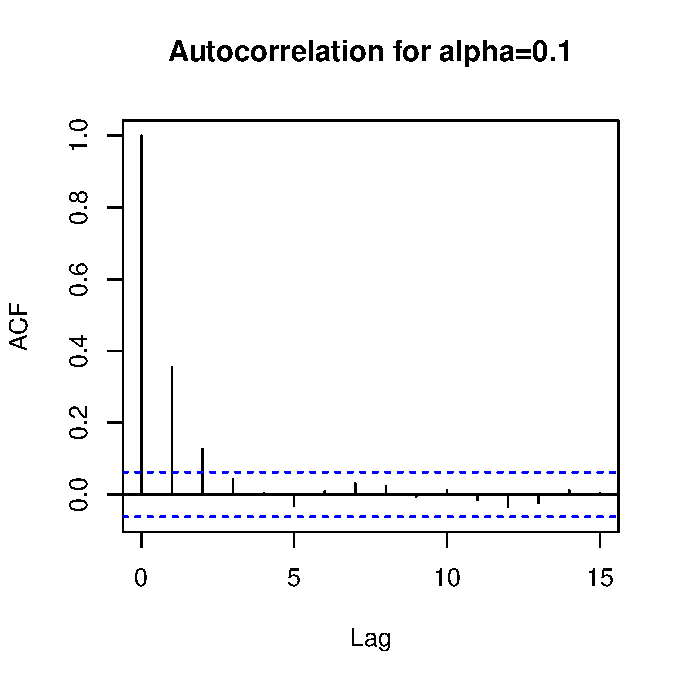
\includegraphics[width=0.44\textwidth]{figures/slice-auto-alpha-optimal}
	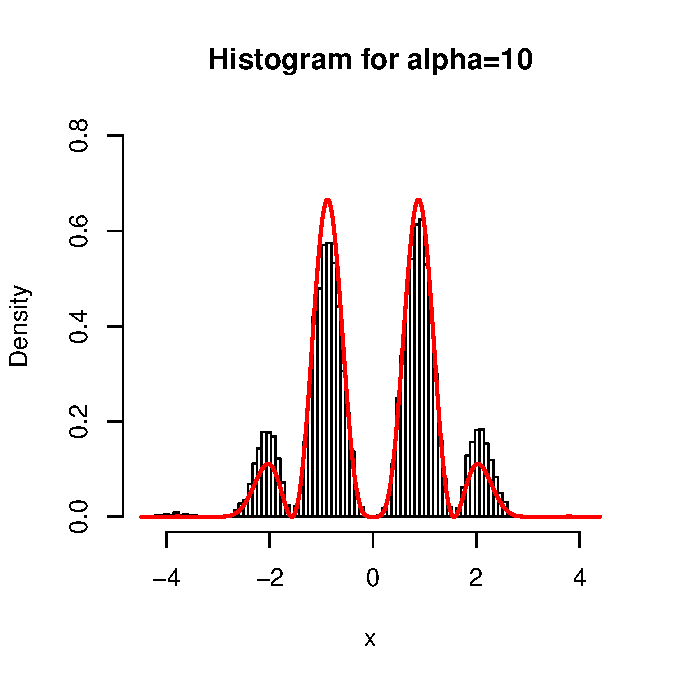
\includegraphics[width=0.44\textwidth]{figures/slice-alpha-big}
	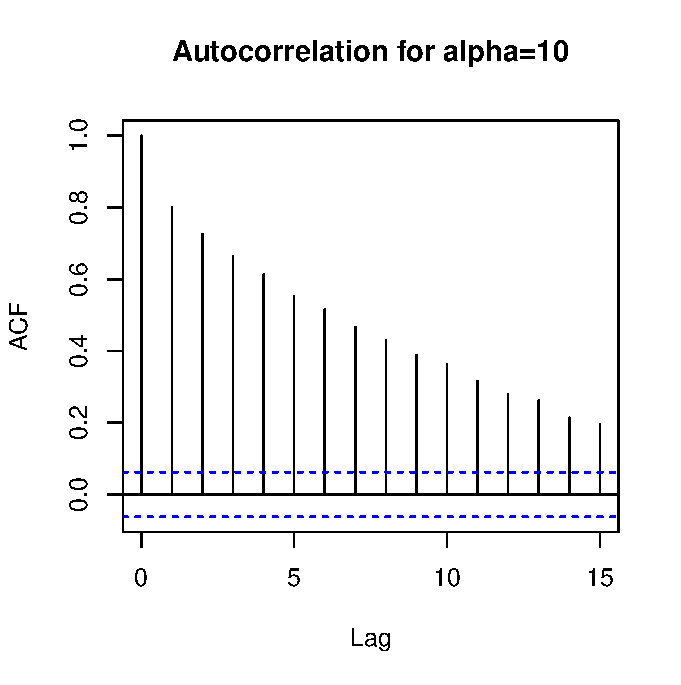
\includegraphics[width=0.44\textwidth]{figures/slice-auto-alpha-big}
	\caption{Histograms and autocorrelation functions for the choices of \(\alpha = 0.01, 0.5, 10\). The auto correlation obviously decreases the fastest for \(\alpha=0.01\), however the computation time is much higher than for the parameter the other parameters.}
	\label{fig:4.3}
\end{figure}
\end{emp}

\subsection{Variational MCMC methods}

Now that we have presented a general setup for MCMC methods we wish to use them to approximated the posterior distribution which is given by the unnormalised density 
\begin{equation}\label{post3}
f(\theta) = f_\Theta(\theta) \prod_{i=1}^n \frac{\det(L(\theta)_{Y_i})}{\det(L(\theta) + I)}.
\end{equation}
In the light of the theoretical guarantees this will surely work and actually Figure \ref{fig:4.1} has been created this way. However, the evaluation of this unnormalised density \(f\) can take several seconds or even minutes itself since it involves the computation of the determinant of the \(N\times N\) matrix \(L(\theta) + I\). However, one can efficiently compute bounds of the unnormalised density and we will provide a general setup of how the MH random walk and slice sampling can be expressed using those bounds. This will lead to significantly shorter simulation times for the respective MCMC methods.

\begin{emp}[Setting]
Let \(\mathcal X\) be a measurable space, \(\mu\) a measure on that space and \(f\colon\mathcal X\to[0, \infty]\) a function with finite positive integral
\[Z = \int\limits_{\mathcal X} f(x) \mu(\mathrm{d}x)\in(0, \infty).\]
Let further \(f\le \left\lVert f \right\rVert_{L^\infty(\mu)}\) and let
\[\left\{ f(\cdot|x) \mid x \in\mathcal X\right\}\]
be a family of proposal distributions.
Let now \(f_n^-, f_n^+\colon\mathcal X\to [0, \infty]\) be functions such that \(f_n^-(x)\le f(x)\le f_n^+(x)\) for all \(x\in\mathcal X\) as well as
\[f_n^\pm(x) \xlongrightarrow{n\to\infty} f(x) \quad \text{for all } x\in\mathcal X. \]
We seek an expression of the MH random walk and the slice sampling method that purely relies on those bounds \(f_n^-\) and \(f_n^+\) of the unnormalised density.
\end{emp}

\subsubsection*{Variational MH random walk}

We note that the only part in the algorithm for the MH random walk where \(f\) is needed itself is the accept-reject step, hence, it suffices to adjust this step. In order to achieve this we bound the acceptance rate through
\[\rho_n^\pm(x, y) \coloneqq \min\left\{ \frac{f_n^\pm(y) f(x|y)}{f_n^\mp(x)f(y|x)}, 1\right\}.\]
In fact we obviously have \(\rho_n^-(x, y)\le\rho(x, y)\le\rho_n^+(x, y)\) as well as
\[\rho_n^\pm(x, y)\xlongrightarrow{n\to\infty}\rho(x, y) \quad\text{for all } x, y\in\mathcal X. \]
Hence if we want to decide whether a number \(a\) satisfies \(a\le \rho(x, y)\) we can iteratively tighten the upper and lower bounds on \(\rho\) until we either have \(a\le\rho_n^-(x, y)\) and thus \(a\le\rho(x, y)\) or \(a>\rho_n^+(x, y)\) and therefore \(a>\rho(x, y)\).
Now we can adjust the algorithm of the MH random walk accordingly and obtain Algorithm \ref{alg:variational-MH}.

\begin{algorithm}
\caption{One step in the variational MH random walk \label{alg:variational-MH}}
\begin{algorithmic}[1]
\Require{Current state \(x_n\) of the MH random walk}
\State \(y\sim f(\cdot|x_n)\mathrm d\mu\)
\State \(a\sim \mathcal U([0, 1])\)
\State \(k\gets 1\)
\While {\(a>\rho_k^-(x_n, y)\) and \(a\le \rho_k^+(x_n, y)\)}
  \State \(k \gets k+1\)
\EndWhile
\If{\(a\le \rho_k^-(x_n, y)\)}
  \State \(x_{n+1}\gets y\)
\Else 
  \State \(x_{n+1}\gets x_n\)
\EndIf
\State\Return{\(x_{n+1}\)}
\end{algorithmic}
\end{algorithm}

\subsubsection*{Variational slice sampling}

In the slice sampling we use the unnormalised density twice. The first time when sampling \(y\sim\mathcal U([0, f(x_n)])\) and the second time when checking \(x\in S(y)\) or equivalently \(f(x)\ge y\). For the first problem we note that we surely have \([0, f(x_n)]\subseteq [0, f_1^+(x_n)]\) and hence we can use Algorithm \ref{alg:slice-sample} to sample uniformly from \([0, f(x_n)]\). However, in this algorithm we need to check \(y\in [0,f(x_n)]\) or equivalently \(f(x_n)\ge y\) which is just what we had to do determine whether \(x\in S(y)\). Therefore, it suffices to see how one can check \(f(x)\ge y\) which we will do analogously to the variational MH random walk by gradually tightening the bounds. This yields Algorithm \ref{alg:decide} that returns �TRUE� if \(f(x)\ge y\) and �FALSE� otherwise.

\begin{algorithm}
\caption{Deciding \(f(x)\ge y\) through the bounds \label{alg:decide}}
\begin{algorithmic}[1]
\Require{\(y\in\mathbb R\) and \(x\in\mathcal X\)}
\State \(k\gets 1\)
\While {\(y>f_k^-(x)\) and \(y\le f_k^+(x)\)}
  \State \(k \gets k+1\)
\EndWhile
\If{\(y\le f_k^-(x_n, y)\)}
  \State \Return{TRUE}
\Else 
  \State \Return{FALSE}
\EndIf
\end{algorithmic}
\end{algorithm}

In conclusion we can express both MCMC methods exactly through those bounds as long as the bounds converge. This enables a fast simulation of the Markov chains if the unnormalised density is slow but the bounds \(f_n^\pm\) are easy to compute. In the case that \(f\) is the posterior \eqref{post3} of a DPP such bounds are given in \cite{affandi2014learning} and \cite{bardenet2015inference}.


% \chapter{Toy examples and experiments}

\section{Minimal example?}

\section{Points on the line}

The first example we present is a selection of points on a (discretised) line. More precisely we will assume that we have \(100\) points on a line that are equally spaced and we aim to model a spacial repulsion between the selected points. For this we will use the method \ref{moddiv} of reference points % \todo{formulate and cite it!} of modelling
 the diversity features. In this case we will use the set \(\mathcal Y\) itself as reference set and use a 

\begin{emp}[Setup of the example]
Let \(\mathcal Y \coloneqq\left\{ 1, \dots, 100\right\}\) and for \(i\in\mathcal Y\). Then we will  let \(\phi_i\in\mathbb R^{100}\) be given up to scaling by
\[(\phi_i)_j\propto f\left(\frac{\left\lvert i - j \right\rvert}{???}\right)\]
where \(f\) is the density of the standard nomal distribution. Further we choose the qualities to be constant and so that the expected cardinatlity is \(10\)\todo{check}.
\end{emp}

\begin{rem}%[Remark]
\begin{enumerate}
\item describe scaling including choice of cardinality
\item describe rank of the kernel?
\item describe choice of �repulsiveness�, plot density around a point; make comment to kernel methods? comment on the qualitative properties of \(f\) and why they are suitable here
\end{enumerate}
% \todo{explain scaling of the quality}
\end{rem}

To make the difference to an uncorrelated point pattern more apparent we also defined a Poisson process, i.e. a DPP without correlations between the points with the same expected cardinality. The sampling results are compared in Figure \ref{fig:4.1}.% Such uncorrelated DPPs are called \emph{Poisson point processes}.\todo{introduce earlier!}

\vspace{2cm}
\begin{figure}[h!]
	\centering
	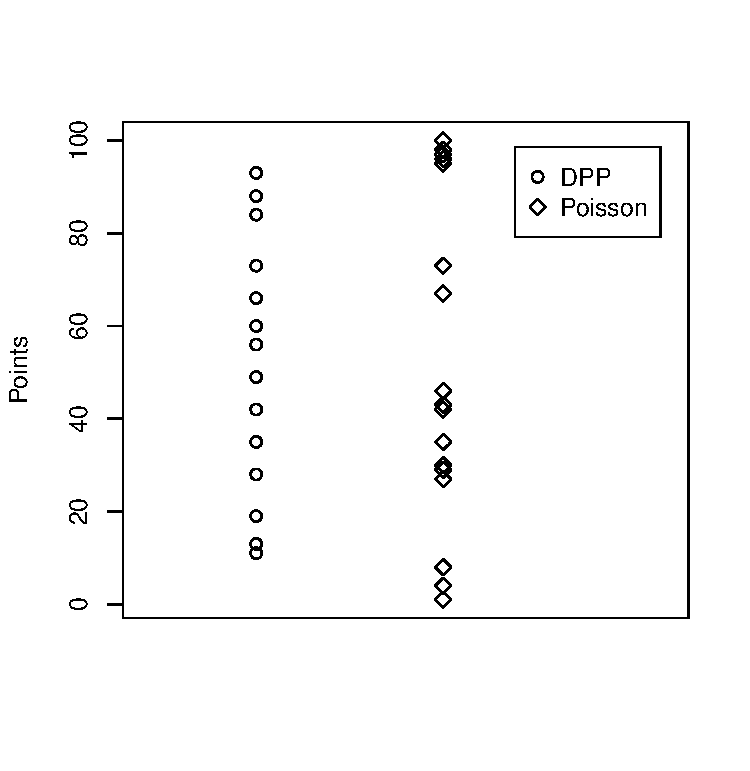
\includegraphics[width=0.6\textwidth]{comparison-dpp-poisson}
%	\tag{1}
	\caption{Comparison of a DPP with negative correlations on the left and no correlations, i.e. a Poisson point process on the right.}
	\label{fig:4.1}
\end{figure}
\todo{make comment on zeta function!}

\begin{emp}[Representation as binary sequence]

\end{emp}
\todo{comment on problems and findings?}
\section{Points in the square}

\section{Toy example for quality learning}

\chapter{Summary and conclusion}

%\todo{General properties first?}
In this thesis we gave a short but mostly self contained introduction to the basic notions of discrete determinantal point processes. This also included results concerning their existence as well as an explicit construction of them which can be used to simulate them.

Based on those preliminaries we have presented different approaches to the estimation of several parametric models of discrete DPPs. First we presented a point estimator that reconstructs an estimation for the marginal kernel according to the empirical marginal densities. The central tool for this is the solution of the principle minor assignment problem that is concerned with the existence and construction of a matrix with prediscribed principle minors. We showed how this can be reduced to the solution of a set of linear equations over the prime field \(\mathbb F_2\). One drawback of this approach is, that one has to calculate a minimal shortest cycle basis of the estimated adjacency graph which is not straight forward to implement. Further we have seen that this estimator is consistent, but the results in \cite{urschel2017learning} also imply that the convergence might be very slow. % which again relies on the 

The second approach was based on the well established theory of maximum likelihood estimation, which yields another point estimator. However the main difficulty here is that the log likelihood function for the whole elementary kernel \(L\) is not concave and therefore hard to maximise in practice. Nevertheless, we have seen that this problem can be solved by the use of a log linear model for the qualities. The trade off is that this model has a lower descriptive power and that one has to model the similarity of the DPP which determines the structure and strength of the repulsion. Finally, we proved that the MLEs exist with increasing probability and that they are consistent estimators for the respective parameters which we also generalised to the MAP estimation. %\todo{add consistency}

In the third chapter we introduced the Bayesian approach to parameter estimation which is fundamentally different in the sense that it treats the estimated parameter as a random varibale rather than a single value. This does not only allow to capture the uncertainty of the estimation but also has a regularising effect in the sense that the posterior distribution always exists even if the according maximum likelihood estimator doesn�t. We have seen that the prior corresponds exactly to the explicit regularisation of the MLE we considered earlier. We have seen how the posterior density of the parameter can be approximated using different MCMC methods even if the MLE is impossible to compute. 

In the last chapter we performed the MLE and Bayesian estimation for a toy model introduced earlier. We saw how the sample size affects the quality of the estimation, in particular with different regularisations. In general, it can be noted that a wrong regularisation is especially bad for small sample sizes and hence different priors should be compared, for example using the Bayes factor. Further we used the MH random walk to approximate the posterior distribution and applied two different burn in periods. It is apparent that the tuning of the proposal lead to a higher acceptance rate and a faster decreasing auto correlation function. Finally we investigated the effect random noise has on the estimation. In fact, some parameters get distorted by the presence of Poisson noise, however we argue that it is only reasonable to use a suitable regulariser if one has a clear understanding of the qualitative structure of this influence.
%\todo{comment on examples and negative effect of regularisation}

%\begin{enumerate}
%\item We�ve seen different approaches to the parameter estimation of DPPs
%\item The first two we�re point estimators and we�ve seen that they are both consistent. However, the maximum likelihood estimation runs into computational problems since one has to maximise a non concave function.
%\item This and also the goal to capture uncertainty and to regularise the parameter estimation -- which will solve the problem that the MLE doesn�t always exist -- lead to the Bayesian approach to parameter estimation. Here the problem is that the normalisation constant of the posterior density can not be computed analytically or numerically. Nevertheless, the posterior density can be approximated through MCMC methods.
%\end{enumerate}�

\subsubsection{Further work}

During the work on this dissertation the following questions arose that might be worth to consider further. 

\begin{enumerate}
\item Can one effectively perform maximum likelihood estimation of the repulsiveness parameter \(\sigma\), in the best case even simultaneously to the log linearity constant \(\theta\) of the quality? If not, could this be done by iteratively optimising \(\sigma\) and \(\theta\) after another? If one of those procedures works theoretically, does it provide any significant improvement over the other estimations?
\item What does the geometry of the log likelihood function of the whole elementary kernel look like? Are there other critical points than to the global maximiser? %as a function of the determinantal equivalence classes? Is there a unique maximiser of the log likelihood function in this case and maybe even a unique critical point? %What is the structure of the set of those equivalence clases and can one effectively optimise functions on this set? %Then standard optimisation tools could be used. However, the structure of those equivalent classes is not obvious....
\item Are the presented point estimators unbiased? 
\item How do the different point estimators perform compared to each other and can one put those findings onto rigorous base in the sense that one is the optimal estimation for some given observations? Does that performance change under the presence of noise?
\item Investigate whether the �naive� approach for the approximation of the posterior could somehow be saved in higher dimension. Past work on the approximation of high dimensional functions could help here as well.
%say something about the grid method.
%Does the regularising effect of the prior bring any substantial benefits if one perturbs the observation with random noise? %How strong and beneficial is the regularising effect of the prior in terms of noise on the observation?
\item Find further applications for the use of DPPs.
\end{enumerate}

To conlude, we want to emphasise that we believe that determinantal point processes will continue to get attention from the research communities concerned with machine learning, data science and computational statistics. We assume that they can help to improve various current techniques in those fields and think that they are already on the way of doing this.  %-- although the focus of this dissertation was the estimation of the parameters of DPPs -- 


\appendix
\renewcommand{\thesection}{\Alph{chapter}.\arabic{section}}
\renewcommand*{\thesatz}{\Alph{chapter}.\arabic{satz}}
\setcounter{section}{0}

% \begin{appendices}
% \setcounter{chapter}{2}

\chapter{Calculations}

\begin{prop}[Complement of DPPs]
Let \(\mathbf Y\) be a random subset that is distributed according to a DPP with marginal kernel \(K\in\mathbb R^{N\times N}\). Then we have
\[\mathbb P(A\subseteq\mathbf Y^c) = \det\big( (I-K)_A\big). \]
Hence the complement \(\mathbf Y^c\) is distributed according to a DPP with marginal kernel \(I-K\).
\end{prop}
\begin{proof}

\end{proof}

\begin{prop}[Normalisation]
Let \(L\in\mathbb R^{N\times N}\) for \(N\in\mathbb N\). Then we have
\[\sum_{A\subseteq [N]} \det(L_A) = \det(L + I) \]
where \([N]\coloneqq\left\{ 1, \dots, N\right\}\).
\end{prop}
\begin{proof}

\end{proof}

\begin{theo}[Cantor�s intersection theorem]
Let \(\mathcal X\) be a topological Hausdorff space and let \(K_1\supseteq K_2\supseteq \dots\) be a sequence of descending, non empty compact sets. Then also the intersection
\[\bigcap_{n=1}^\infty K_n\]
is non empty.
\end{theo}
\begin{proof}
Assume that the intersection would be empty, and set \(U_n\coloneqq \mathcal X\setminus K_n\) which is open since \(K_n\) is closed as the compact subset of a Hausdorff space. Then \((U_n)_{n\in\mathbb N}\) is an open covering of \(K_1\) since we have
\[\bigcup_{n=1}^\infty U_n = \mathcal X\setminus\left( \bigcap_{n=1}^\infty K_n\right) = \mathcal X. \]
Hence we can select a finite subcover and obtain
\[K_1\subseteq \bigcup_{n=1}^N U_n = \mathcal X\setminus \left( \bigcap_{n=1}^N K_n\right) = \mathcal X\setminus K_N.\]
However since \(K_n\subseteq K_1\) this implies \(K_N = \varnothing\) which is a contradiction.
\end{proof}

\chapter{Generated code}

All my coding was done in R and I will provide the code for sampling, my examples and also the learning algorithm of my toy example here. During my coding I mostly followesd Google�s R Style Guide (https://google.github.io/styleguide/Rguide.xml).

% Some text

% \chapter{bla title}
% Some text
% \subsection{foo title}
% Some text

\section{Sampling algorithm}

\begin{lstlisting}[language=R, basicstyle=\footnotesize] % , commentstyle=\texttt] %, keywordstyle=\textrm]

# Implementation of the sampling algorithm as a function

SamplingDPP <- function (lambda, eigenvectors) {
  # First part of the algorithm, doing the selection of the eigenvectors
  N = length(lambda)
  J <- runif(N) <= lambda/(1 + lambda)
  k <- sum(J)
  V <- matrix(eigenvectors[, J], nrow=N)
  Y <- rep(0, k)
  
  # Second part of the algorithm, the big while loop
  while (k > 0) {
    # Calculating the weights and selecting an item i according to them
    wghts <- k^(-1) * rowSums(V^2)
    i <- sample(N, 1, prob=wghts)
    Y[k] <- i
    if (k == 1) break
    
    # Projecting e_i onto the span of V
    help <- V %*% V[i, ]
    help <- sum(help^2)^(-1/2) * help
    
    # Projecting the elements of V onto the subspace orthogonal to help
    V <- V - help %*% t(t(V) %*% help)
    
    # Orthonormalize V and set near zero entries to zero
    V[abs(V) < 10^(-9)] <- 0
    j <- 1
    while(j <= k) {
      help2 <- rep(0, N)
      m <- 1
        while (m <= j - 1) {
        help2 <- help2 + sum(V[, j] * V[, m]) * V[, m]
        m <- m + 1
      }
      V[, j] <- V[, j] - help2
      if (sum(V[, j]^2) > 0) {
        V[, j] <- sum(V[, j]^2)^(-1/2) * V[, j]
      }
      j <- j + 1
    }
    V[abs(V) < 10^(-9)] <- 0
    
    # Selecting a linear independent set in V
    k <- k - 1
    q <- qr(V)
    V <- matrix(V[, q$pivot[seq(k)]], ncol=k)
  }
  return(Y)
}
\end{lstlisting}

\section{Points on the line}

\begin{lstlisting}[language=R, basicstyle=\footnotesize]

# NEEDS: sampling algorithm

# In this example we sample points on a (discrete) line according to a DPP
# We model L directly and via the quality-diversity decomposition. We plot and
# compare the patterns to uncorrelated points i.e. to a Poisson point process.

# Minimal example _____________________________________________________________
n <- 3
L <- matrix(c(2,1,0,1,2,0,0,0,2), nrow=n)

# Points on a line ____________________________________________________________
n <- 100
L <- rep(0, n^2)
for (i in 1:n) {
  for (j in 1:n) {
    L[(i - 1) * n + j] <- dnorm((i-j) * n^(-1/4))
  }
}
L <- matrix(L, nrow=n)

# Modelling phi and q _________________________________________________________
# Points on the line.
m <- 99  # 29
n <- m + 1
q <- rep(10, n)  # 0-1 sequences: rep(10^2, n)
phi <- rep(0, n^2)
for (i in 1:n) {
  for (j in 1:n) {
    phi[(i - 1) * n + j] <- dnorm((i - j) / 10)  # 0-1 sequences: devide by 2
  }
}
phi <- matrix(phi, ncol=n)

# Log linear quality for the points on the line _______________________________
m <- 99
n <- m + 1
q <- rep(0, n)
for (i in 1:n) {
  q[i] <- 10^2 * sqrt(m) * exp(-0.2 * abs(i - 50.5))
}
phi <- rep(0, n^2)
for (i in 1:n) {
  for (j in 1:n) {
    phi[(i - 1) * n + j] <- dnorm(2 * (i - j) / sqrt(m))
  }
}
phi <- matrix(phi, ncol=n)

# General part, define L ______________________________________________________
for (i in 1:n) {
  phi[, i] <- sum(phi[, i]^2)^(-1/2) * phi[, i]
}
S <- t(phi) %*% phi
time <- proc.time()
L <- t(q * S) * q
proc.time() - time

# Compute the eigendecomposition, set near zero eigenvalues to zero and
# set up poisson point process with same expected cardinality _________________
time <- proc.time()
edc <- eigen(L)
lambda <- edc$values
lambda[lambda < 10^(-9)] <- 0
mean <- sum(lambda / (1 + lambda))
eigenvectors <- edc$vectors
lambda2 <- rep(mean / n / (1 - mean / n), n)
eigenvectors2 <- diag(rep(1, n))
proc.time() - time

# Sample and plot things ______________________________________________________
# Minimal example

# 0-1 sequences
x <- sort(SamplingDPP(lambda, eigenvectors))
as.integer(1:n %in% x)
y <- sort(SamplingDPP(lambda2, eigenvectors2))
as.integer(1:n %in% y)

# Sample from both point processes and plot the points on the line
pointsDPP <- SamplingDPP(lambda, eigenvectors)
pointsPoisson <- SamplingDPP(lambda2, eigenvectors2)
plot(rep(1, length(pointsDPP)), pointsDPP,
     ylim=c(1, n), xlim=c(.4, 3.2), xaxt='n', ylab="Points", xlab="")
points(rep(2, length(pointsPoisson)), pointsPoisson, pch=5)
legend("topright", inset=.05, legend=c("DPP", "Poisson"), pch=c(1, 5))

# Remove all objects apart from functions
rm(list = setdiff(ls(), lsf.str()))

\end{lstlisting}

\section{Points in the square}

\begin{lstlisting}[language=R, basicstyle=\footnotesize]

# NEEDS: sampling algorithm

# In this example we sample points on a two dimensional grid according to a DPP
# We model L directly and via the quality-diversity decomposition including
# different dimensions D for the feature vectors phi. We plot and compare the
# patterns to uncorrelated points i.e. to a Poisson point process.

# Define the coordinates of a point ___________________________________________
CoordinatesNew <- function(i, n) {
  y1 <- floor((i - 1) / (n + 1))
  x1 <- i - 1 - (n + 1) * y1
  return (t(matrix(c(x1, y1)/n, nrow=length(i))))
}
DistanceNew <- function (i, j, n, d) {
  return (sqrt(colSums((CoordinatesNew(i, n) - CoordinatesNew(j, d))^2)))
}

# Direct modelling of L _______________________________________________________
m <- 19
n <- (m + 1)^2
L <- rep(0, n^2)
for (i in 1:n) {
  for (j in 1:n) {
    L[(i - 1) * n + j] = n^2 * dnorm(Distance(i, j, m))
  }
}
L <- matrix(L, nrow=n)

# Modelling phi and q _________________________________________________________
# Points in the square.
m <- 19
n <- (m + 1)^2
q <- rep(sqrt(m), n)
x <- ceiling(1:n^2 / n)
y <- rep(1:n, n)
time <- proc.time()
phi <- dnorm(sqrt(m) *matrix(DistanceNew(x, y, m, m), n))
proc.time() - time

# Quality diversity decomposition with small D ________________________________
d <- 25
q <- rep(10^5 * sqrt(m), n)
x <- ceiling(1:(n*d) / d)
y <- rep(1:d, n)
time <- proc.time()
phi <- dnorm(2 * sqrt(m) * matrix(DistanceNew(x, y, m, sqrt(d) - 1), ncol=n))
proc.time() - time

# Log linear quality for the points in the square _____________________________
m <- 39
n <- (m + 1)^2
q <- exp(-6 * DistanceNew(rep(5, n), 1:n, 2, m) + log(sqrt(m)))
x <- ceiling(1:n^2 / n)
y <- rep(1:n, n)
time <- proc.time()
phi <- dnorm(2 * sqrt(m) * matrix(DistanceNew(x, y, m, m), n))
proc.time() - time


# General part, defining L ____________________________________________________
# d <- length(phi) / n
for (i in 1:n) {
  phi[, i] <- sum(phi[, i]^2)^(-1/2) * phi[, i]
}
S <- t(phi) %*% phi
# B <- t(phi) * q
time <- proc.time()
L <- t(t(q * S) * q)  # B %*% t(B)
proc.time() - time

# Compute the eigendecomposition, set near zero eigenvalues to zero and
# set up poisson point process with same expected cardinality _________________
time <- proc.time()
edc <- eigen(L)
lambda <- edc$values
lambda[abs(lambda) < 10^(-9)] <- 0
mean <- sum(lambda / (1 + lambda))
eigenvectors <- edc$vectors
lambda2 <- rep(mean / n / (1 - mean / n), n)
eigenvectors2 <- diag(rep(1, n))
proc.time() - time

# Sample from both point processes and plot the points in the square __________
# par(mfrow = c(1,1))
time <- proc.time()
dataDPP <- sort(SamplingDPP(lambda, eigenvectors))
pointsDPP <- t(CoordinatesNew(dataDPP, m))
plot(pointsDPP, xlim=0:1, ylim=0:1, xlab="", ylab="", xaxt='n', yaxt='n', asp=1)
proc.time() - time
dataPoisson <- sort(SamplingDPP(lambda2, eigenvectors2))
pointsPoisson <- t(CoordinatesNew(dataPoisson, m))
plot(pointsPoisson, xlim=0:1, ylim=0:1, xlab="", ylab="",
					xaxt='n', yaxt='n', asp=1)

# Remove all objects apart from functions
rm(list = setdiff(ls(), lsf.str()))
\end{lstlisting}

\section{Toy learning example}

\begin{lstlisting}[language=R, basicstyle=\footnotesize]
# NEEDS: Sampling algorithm, declaration of the points in the square
# TODO: Maybe do the gradient descent directly over the representation
# od the gradient

# With this toy example we aim to perform the first learning of paramters
# associated to a kernel of a DPP. More precisely we will generate our own
# data of points on a two dimensional grid with a log linear quality model
# and aim to estimate the log linearity parameter.

# Generation of data
time <- proc.time()
T <- 30
data <- rep(list(0), T)
for (i in 1:T) {
  data[[i]] <- sort(SamplingDPP(lambda, eigenvectors))
}
proc.time() - time

# Define the quality q, L, the feature sum and the loss in dependency of the
# parameter theta
Quality <- function(theta) {
  return(exp(theta[1] * DistanceNew(rep(5, n), 1:n, 2, m) + theta[2]))
}
LFunction <- function(theta) {
  return(t(t(Quality(theta) * S) * Quality(theta)))
} 
Feature <- function(A) {
  # return(sum(DistanceNew(rep(5, length(A)), A, 2, m)))
  return(c(sum(DistanceNew(rep(5, length(A)), A, 2, m)), length(A)))
}
Loss <- function(theta) {
  T <- length(data)
  # Sum this over all data entries
  x <- 0
  for (i in 1:T) {
    A <- data[[i]]
    x <- x + 2 * sum(theta * Feature(A)) + log(det(matrix(S[A, A], length(A))))
  }
  return(- x + T * log(det(diag(rep(1, n)) + LFunction(theta))))
}

# Parameter estimations
time <- proc.time()
sol <- nlm(Loss, c(-3, 0))
proc.time() - time
sol$estimate

# Remove all objects apart from functions
rm(list = setdiff(ls(), lsf.str()))
\end{lstlisting}



\clearpage
\nocite{*}
\bibliographystyle{alpha} %apalike, plain
\bibliography{thesis}
\addcontentsline{toc}{chapter}{Bibliography}

\end{document}